%!TEX root = these.tex

\chapter[Sélection de cibles mobiles : applications]{Sélection de cibles mobiles : quels domaines et quelles applications ?}

\minitoc
\label{chap1}
\cleardoublepage

	\section{Introduction}
	La sélection de cibles est une tâche omniprésente en interaction homme-machine. Si la sélection de cibles mobiles est moins répandue, elle demeure courante, mais assez peu étudiée, cette tache étant plus difficile, selon la nature du mouvement des cibles. En effet, si les cibles mobiles peuvent être décrites par les caractéristiques classiques des cibles statiques, c'est à dire une taille, une forme et une position, s'ajoutent des caractéristiques de mouvement, direction, vitesse,  accélération, et qui peuvent de plus varier dans le temps. 
	
	D'un point de vue perceptif, un utilisateur peut trouver un mouvement plutôt rectiligne, légèrement courbé, très saccadé, circulaire. La grande diversité des types de mouvements perçus, souvent reliés à des mouvements relatifs à l'expérience écologique de l'utilisateur, implique des difficultés à établir  des protocoles expérimentaux permettant de caractériser la difficulté de sélection de cibles mobiles. En effet, il est nécessaire d'apporter des solutions  adaptées aux différentes natures du mouvement des objets à sélectionner. Un des objectifs de ce chapitre est de dégager les grandes lignes de cette diversité de types de mouvements.
	
	Dans ce chapitre introductif, nous nous attacherons à dresser un inventaire des applications impliquant la sélection de cibles mobiles comme tâche durant l'activité. Nous analyserons les enjeux de la sélection dans chacun des cas, afin de comprendre les priorités et besoins spécifiques à chaque application.
	
	Il va sans dire que cet inventaire ne saurait prétendre à l'exhaustivité, tant ces applications sont nombreuses. À défaut d'exhaustivité, l'objectif que nous nous sommes fixés est la représentativité, afin de se forger une idée générale des besoins, des difficultés et enjeux de la sélection de cibles mobiles. Nous verrons que les applications vont des simulations moléculaires aux jeux vidéo, en passant par le contrôle de la circulation aérienne, maritime, terrestre, ainsi que la télévision interactive et divers domaines de la sécurité et de la défense. Une attention plus particulière est volontairement portée sur la description de l'activité de simulation moléculaire interactive, les problématiques de sélection liées à cette activité étant à la base de ce travail de thèse sur la sélection de cibles mobiles.
	

	\section{Simulation moléculaire interactive}
	Avant de décrire l'activité de simulation moléculaire interactive et ses objectifs, il convient de décrire le domaine sous-jacent, c'est-à-dire la biologie moléculaire ou structurale. 
	La biologie structurale est la branche de la biologie qui étudie la structure, l'organisation spatiale, et la dynamique des macromolécules biologiques, principalement les protéines et les acides nucléiques. Elle concerne en particulier la détermination à l'échelle nanoscopique des structures tridimensionnelles de ces molécules et complexes moléculaires (au moyen de techniques biophysiques), les principes à la base des modifications de conformation des macromolécules, l'analyse des mouvements moléculaires et la dynamique de ces structures.

La compréhension moléculaire et structurale du mode d'action d'une molécule sur une autre (ou sur un complexe moléculaire), que des techniques de visualisation aident à appréhender, permet de modéliser les interactions qui se déroulent en permanence à l'échelle moléculaire au sein des organismes vivants.

De même, cette compréhension permet de rationaliser la conception et l'amélioration de molécules actives, de médicaments. On utilise pour cela à la fois des méthodes expérimentales d'analyse structurale, mais aussi des approches computationnelles pour prédire des candidats médicaments à partir de la structure.

Nous allons voir dans cette section que les approches computationnelles se fondent notamment sur des simulations qui, lorsqu'elles sont interactives, nécessitent la sélection de cibles mobiles particulièrement difficiles à saisir. Cette difficulté est la première motivation des travaux présentés dans ce manuscrit.
	
	\FloatBarrier \subsection{Contexte de la dynamique moléculaire}
	Une simulation de dynamique moléculaire~\cite{fermi1955alamos, alder1959studies, rahman1964correlations, gibson1960dynamics, lennard1924determination} consiste à simuler, par un calcul numérique, le comportement d'un système moléculaire dans le temps. Celui-ci est modélisé par un système de particules, avec généralement une particule par atome. Des formules mathématiques permettent de modéliser les différentes forces qui s'appliquent à chaque particule, et ces forces sont intégrées avec un pas de temps pour déterminer le mouvement de chaque particule à chaque itération, donc la dynamique du système.
	
	\subsubsection{Besoins} Il est difficile d'observer une macromolécule à l'état statique, et impossible de le faire \emph{in vivo}, lorsqu'elle est en mouvement dans son système naturel. Par conséquent, l'étude de phénomènes moléculaires complexes nécessite de passer par des simulations numériques, seules à même d'en rendre compte. En particulier, la biologie structurale s'intéresse à la \emph{dynamique conformationnelle} des macromolécules (c'est-à-dire à leur conformation tridimensionnelle dans le temps) et à leurs interactions avec leur environnement --- par exemple le milieu cellulaire. Ces simulations sont devenues fiables en s'appuyant autant que possible sur des données expérimentales.
	
	\subsubsection{Initialisation}
	Une simulation de dynamique moléculaire nécessite une phase d'initialisation : on assigne une position à chaque particule. Pour ce faire, il est nécessaire de connaître au moins approximativement la conformation de chaque molécule du système. C'est relativement simple pour le solvant (le fluide dans lequel la molécule se trouve --- généralement de l'eau), mais c'est plus compliqué pour les macromolécules dont la conformation est complexe. Celle-ci est généralement déterminée par une méthode expérimentale telle que la cristallographie aux rayons X, illustrée par la figure~\ref{fig:crystal}. Cette technique fut d'abord employée pour déterminer la structure de petits cristaux inorganiques~\cite{friedrich1912sitzungsberichte, bragg1914reflexion, bragg1913structure, dickinson1923crystal}, puis de molécules organiques et de protéines*~\cite{de1925interpretation, crowfoot1935x, kendrew1958three}\footnotemark{}. Lorsque la cristallographie n'est pas possible, d'autres méthodes, souvent moins précises, peuvent être utilisées. Citons la spectroscopie de résonance magnétique nucléaire~\cite{clore1989determination, wuthrich1990protein, clore1991structures, wuthrich2001way}, ou la cryo-microscopie électronique~\cite{adrian1984cryo} (cryo-ME/\emph{cryo-EM}), de plus en plus utilisée~\cite{kuhlbrandt2014cryo, callaway2015revolution, dellisanti2015barrier, bartesaghi20152}.

	\footnotetext{Les notions évoquées dans cette section et suivies d'un astérisque sont définies et détaillées dans l'annexe~\ref{appendix:annexeA}.}
	
	Parfois, on procède également par homologie~\cite{marti2000comparative, kaczanowski2010similar}. Ce procédé repose sur l'identification d'une ou plusieurs structures protéiques* connues et proches de la séquence d'acides aminés* recherchée. Elle passe par un alignement qui établit une correspondance entre les acides aminés de la protéine étudiée et ceux des structures protéiques connues. Cela s'appuie sur l'observation que la structure tridimensionnelle de protéines homologues est mieux conservée que la séquence d'ADN* qui l'engendre. La connaissance de la séquence d'acides aminés d'une protéine permet donc d'essayer de prédire sa conformation 3D, si l'on parvient à trouver des protéines homologues dont la structure est connue.
	
	\begin{figure}[!htbp]
		\centering
		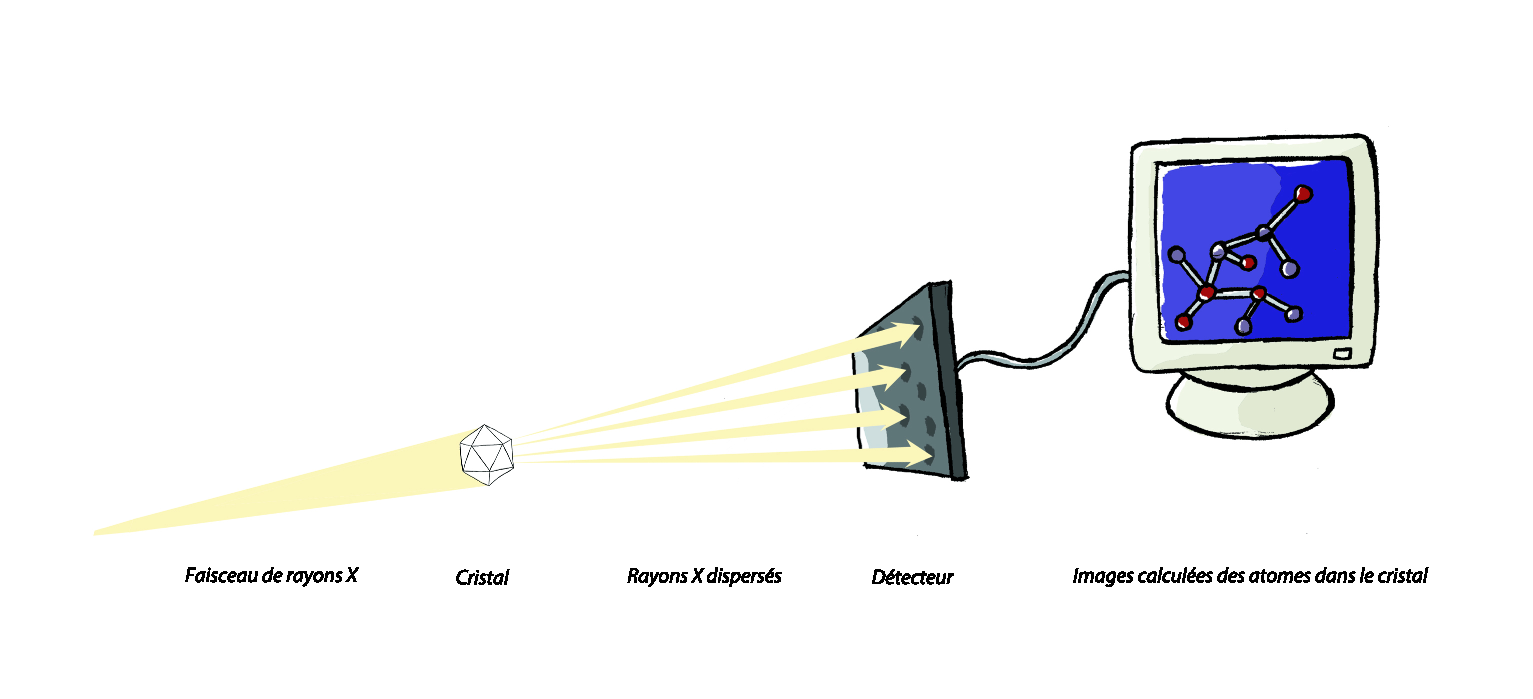
\includegraphics[width=\textwidth]{figures/ch1/crystal}
		\caption[Schéma très simplifié de la cristallographie aux rayons X]{Schéma très simplifié de la cristallographie aux rayons X. Ces rayons traversent un cristal (contenant une même molécule présente en grande quantité) qui les diffracte avant leur capture par un détecteur connecté à un ordinateur. Ce dernier, à l'aide d'un algorithme approprié, en déduit la conformation 3D de la molécule cristallisée. Crédit :~\cite{trellet2015exploration}.}
		\label{fig:crystal}
	\end{figure}
	
	\subsubsection{Périodicité}
	L'espace de simulation est généralement modélisé par ce qu'on appelle des conditions périodiques aux limites~\cite{cheatham1995molecular} (CPL, en anglais \emph{periodic boundary conditions} --- PBC). Elles constituent un ensemble de conditions aux limites utilisées afin de simuler un système pavé effectivement infini. En effet, si un système microscopique est simulé dans le vide, les molécules du système s'évaporeront, s'éloignant les unes des autres à moins d'être maintenues ensemble par une force restrictive externe. Si, au contraire, le système est simulé en utilisant des murs réflecteurs aux limites, des forces parasites sont introduites dans la simulation, pouvant donc créer un écart supplémentaire (en plus des approximations de simulation utilisées) par rapport au système réel.
	
	On optera donc généralement pour un système périodique. Il convient toutefois de prendre des précautions avec les conditions périodiques, afin d'éviter que des interactions \og artificielles \fg{} se produisent entre les \og bords \fg{} de l'espace de simulation, notamment entre les particules et leurs propres images si cela ne correspond pas au système étudié dans son état naturel~\cite{de1997effect}. L'utilisation de formes plus complexes que des parallélépipèdes peut permettre de minimiser ces effets indésirables pour un volume de simulation donné ; les octaèdres tronqués sont une des options possibles, comme l'illustre la figure~\ref{fig:octa}.
	
	\begin{figure}[!htbp]
		%\centering
		\begin{subfigure}{.49\textwidth}
			\centering
			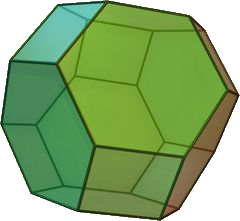
\includegraphics[height=4cm]{./figures/ch1/truncOctahedron}
			\caption{Octaèdre tronqué.}
			\label{fig:truncOctahedron}
		\end{subfigure}
		~
		\begin{subfigure}{.49\textwidth}
			\centering
			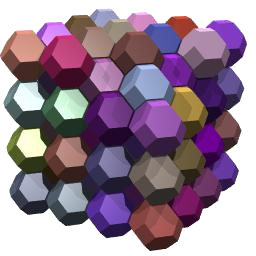
\includegraphics[height=4cm]{./figures/ch1/truncOctahedra}
			\caption{Treillis d'octaèdres tronqués.}
			\label{fig:truncOctahedra}
		\end{subfigure}
		\caption[Octaèdres pour les conditions périodiques aux limites]{Utilisation d'octaèdres pour la mise en œuvre de conditions périodiques aux limites en minimisant les erreurs et les calculs nécessaires. Crédit : S.R. Saunders, \emph{Real Wireless}\footnotemark.}
		\label{fig:octa}
	\end{figure}
	
	\footnotetext{\url{https://realwireless.wordpress.com/2008/06/03}}
	
	\subsubsection{Paramètres initiaux} Le principe de la simulation est de calculer les forces exercées sur chaque particule à chaque itération, et d'intégrer ces forces sur un pas de temps donné pour déplacer les particules. Pour pouvoir simuler le comportement du système sur un temps assez long --- afin d'observer des phénomènes biologiques complexes et longs --- le pas de temps doit être aussi grand que possible.
	
	Cependant, il doit être suffisamment court pour que les événements les plus rapides ne soient pas perdus. Or, les oscillations des liaisons covalentes*, par exemple, sont très courtes, de l'ordre de $10^{-14}$~s, soit 10~fs\footnotemark{}. Le théorème de Nyquist-Shannon~\cite{shannon1949communication} nous apprend qu'il est nécessaire que la fréquence d'échantillonage soit au moins le double de la fréquence du signal, aussi le pas de temps doit-il être, au plus, deux fois plus court que la période d'une oscillation de liaison covalente. En pratique, la valeur choisie est généralement de l'ordre de $10^{-15}$~s, soit 1~fs pour les simulations les plus précises.
	
	\footnotetext{Une femtoseconde (fs) vaut $10^{-15}$ seconde.}
	
	D'autres paramètres doivent être initialisés : les vitesses des particules, (généralement selon une distribution de Maxwell-Boltzmann~\cite{maxwell1860v, maxwell1860ii, boltzmann1970weitere, boltzmann2003further}), la température, la pression, le nombre de particules, etc. Le changement d'un seul de ces paramètres mènera généralement à une autre exploration de l'espace conformationnel, c'est-à-dire à une trajectoire différente.
	
	\subsubsection{Champs de force}
	Une simulation de dynamique moléculaire s'appuie sur un \emph{champ de force}. Cette notion, propre à la chimie, est à ne pas confondre avec son homonyme en physique. Ce que l'on appelle ici un champ de forces est un ensemble de potentiels et de paramètres permettant de modéliser les interactions entre les particules simulées. Généralement, la forme fonctionnelle de base d'un champ de force s'appuie sur l'équation suivante (également illustrée par la figure~\ref{fig:ffterms}) :
	
	\begin{equation}
		\label{eq:forcefield}
		E_{totale} = E_\text{liée} + E_\text{non-liée}
	\end{equation}
	
	\begin{figure}[!htbp]
		\centering
		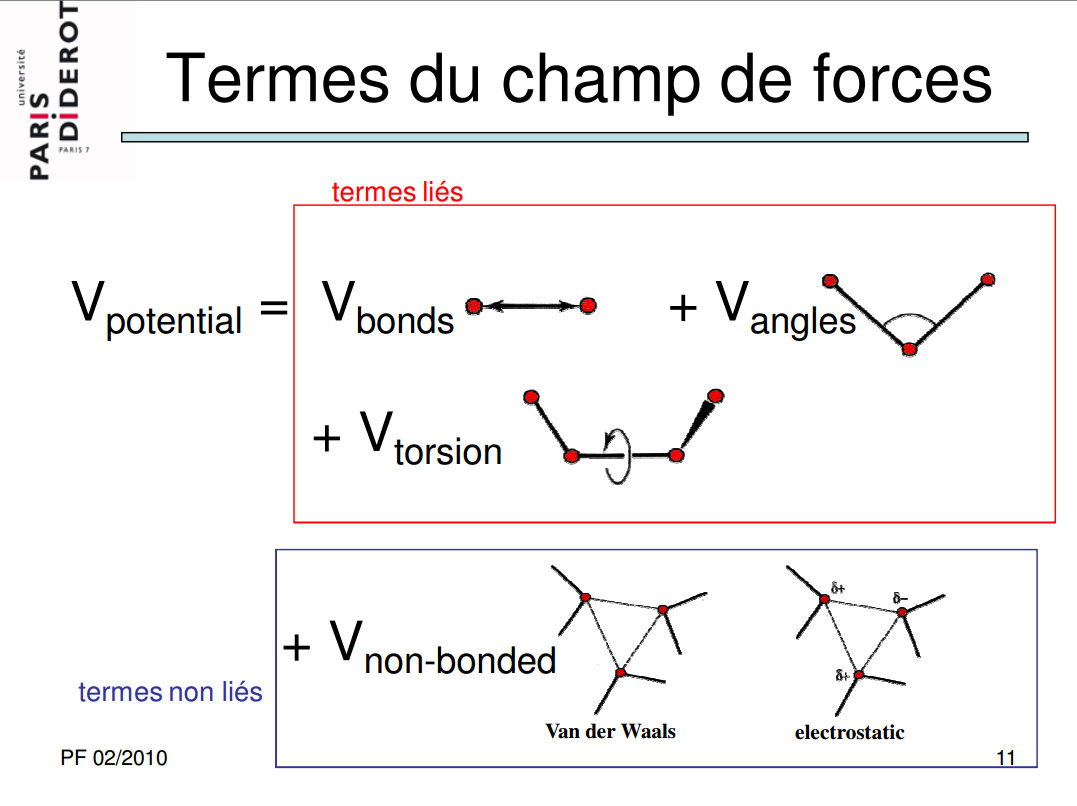
\includegraphics[width=\textwidth]{figures/ch1/ffterms}
		\caption[Termes d'un champ de forces]{Résumé des termes liés et non liés d'un champ de forces typique. Crédit : Patrick Fuchs\footnotemark.}
		\label{fig:ffterms}
	\end{figure}
	
	\footnotetext{\url{http://www.dsimb.inserm.fr/~fuchs/M1BC2T/Cours1_FF.pdf}}
	
	L'énergie totale est égale à l'énergie liée plus l'énergie non-liée, où l'énergie liée représente l'énergie des liaisons covalentes, et l'énergie non-liée représente toutes les autres interactions.
	
	\begin{equation}
		\label{eq:ebonded}
		E_\text{liée} = E_{liaison} + E_{angle} + E_\text{angle\_{}dièdre}
	\end{equation}
	
	Le terme $E_{liaison}$ correspond à l'énergie associée à la variation de la longueur d'une liaison covalente par rapport à son équilibre.%, comme l'illustre la figure~\ref{fig:e_bond}.
	
	Le terme $E_{angle}$ représente l'énergie associée à la déformation des angles formés par les paires de liaisons covalentes impliquant le même atome.% cf. la figure~\ref{fig:e_angle}.
	
	Le terme $E_\text{angle\_{}dièdre}$ correspond à l'énergie associée à la \og torsion \fg{} des liaisons covalentes centrales dans des groupes de quatre atomes.
	
	\begin{equation}
		\label{eq:nonbonded}
		E_\text{non-liée} = E_\text{électrostatique} + E_{van der Waals}
	\end{equation}
	
	Le terme $E_\text{électrostatique}$ représente l'énergie des interactions électrostatiques entre les paires d'atomes ne partageant pas de liaison covalente, telle que la décrit la loi de Coulomb~\cite{coulomb1785premier}.
	En pratique, une sommation d'Ewald, basée sur une transformation de Fourier, est souvent utilisée avec la loi de Coulomb pour le calcul des énergies électrostatiques~\cite{ewald1921berechnung, essmann1995smooth}.
	
	Le terme $E_\text{van der Waals}$ correspond à l'énergie associée aux forces de van der Waals*.
	
	Il existe de très nombreux champs de force, avec chacun ses avantages et inconvénients spécifiques, mais parmi les plus couramment utilisés, on peut citer \emph{Chemistry at HARvard Molecular Mechanics} (CHARMM)~\cite{brooks1983charmm, brooks2009charmm}, \emph{Assisted Model Building and Energy Refinement} (AMBER)~\cite{cornell1995second, wang2004development}, \emph{Optimized Potential for Liquid Simulations} (OPLS)~\cite{jorgensen1996development, kaminski2001evaluation}, ou encore \emph{GROningen MOlecular Simulation} (GROMOS)~\cite{scott1999gromos, oostenbrink2004biomolecular}.
	
    
	\FloatBarrier \subsection{Problématique des simulations interactives}
	
	\subsubsection{Limites des simulations non interactives}
	Les processus biologiques dont l'étude nécessite l'emploi de simulations de dynamique moléculaire impliquent souvent des événements relativement longs ou rares, tels que de profonds changements de conformation, ou des transitions d'un état d'équilibre à un autre, comme la liaison ou la rupture de liaison avec un ligand*. Or, les simulations de dynamique moléculaire étant généralement limitées à quelques dizaines de nanosecondes, ces phénomènes ne sont pas toujours observables ou reproductibles~\cite{phillips2005scalable}.
	
	\subsubsection{Steering}
	Par conséquent, il est utile de pouvoir agir sur une simulation de dynamique moléculaire. Cette technique est souvent appelée \emph{steering} dans la littérature anglo-saxonne et consiste à appliquer des forces externes à une molécule au cours de sa simulation pour explorer ses propriétés mécaniques, ou pour chercher à provoquer les phénomènes mentionnés ci-dessus, trop lents pour les simulations sans \emph{steering}. Ces phénomènes peuvent ainsi être étudiés~\cite{izrailev1999steered, isralewitz2001steered, isralewitz2001steered}. Certains spécialistes~\cite{phillips2005scalable} préfèrent parler d'\emph{Interactive Molecular Dynamics} (IMD)~\cite{stone2001system, grayson2003mechanisms} lorsque les forces sont appliquées en temps réel par l'utilisateur, par opposition au \emph{steering} fondé sur des forces dont l'application est préprogrammée. L'interactivité permet aussi de trouver des conformations 3D d'acides nucléiques plus rapidement, même avec des utilisateurs novices~\cite{mazzanti2017can}, et offre à l'utilisateur la possibilité d'intervenir pendant la simulation.
	
	\subsubsection{Simulations en immersion}
	La figure~\ref{fig:steeredPIT} présente un exemple précoce (1999) d'IMD en contexte immersif. La notion d'immersion fait l'objet de plusieurs définitions, notamment celle citée par J.-M.~Burkhardt \emph{et al.}~\cite{burkhardt2003immersion} :
	
	\begin{displayquote}
		Dans le langage courant, le terme d'immersion est compris comme \emph{l'exposition de l'utilisateur à un [environnement virtuel (EV)] au moyen de dispositifs occultant en partie la perception} (surtout visuelle) de l'environnement alentour, pour afficher en lieu et place une image du monde virtuel (visio-casque, salle immersive de type CAVE, etc.). Par extension, on parle d'immersion auditive, haptique, sensorielle etc. Au-delà d'un caractère informel, cette acception comporte deux ambiguïtés. D'une part, deux sémantiques différentes coexistent :
	    \begin{enumerate}
	        \item l'immersion comme \emph{l'action d'exposer l'utilisateur à un environnement simulé numériquement},
	        \item l'effet avéré ou supposé de cette exposition sur l'utilisateur.
	    \end{enumerate}
	    
	    D'autre part, en se focalisant sur l'aspect d'exposition, cet usage courant tend à centrer le problème sur la recréation d'une image artificielle proche de la situation réelle de référence, et à occulter les éventuelles interactions avec l'information persistante liée à l'environnement physique réel de l'utilisateur.	    
	\end{displayquote}
	
	\begin{figure}[!htbp]
		\centering
		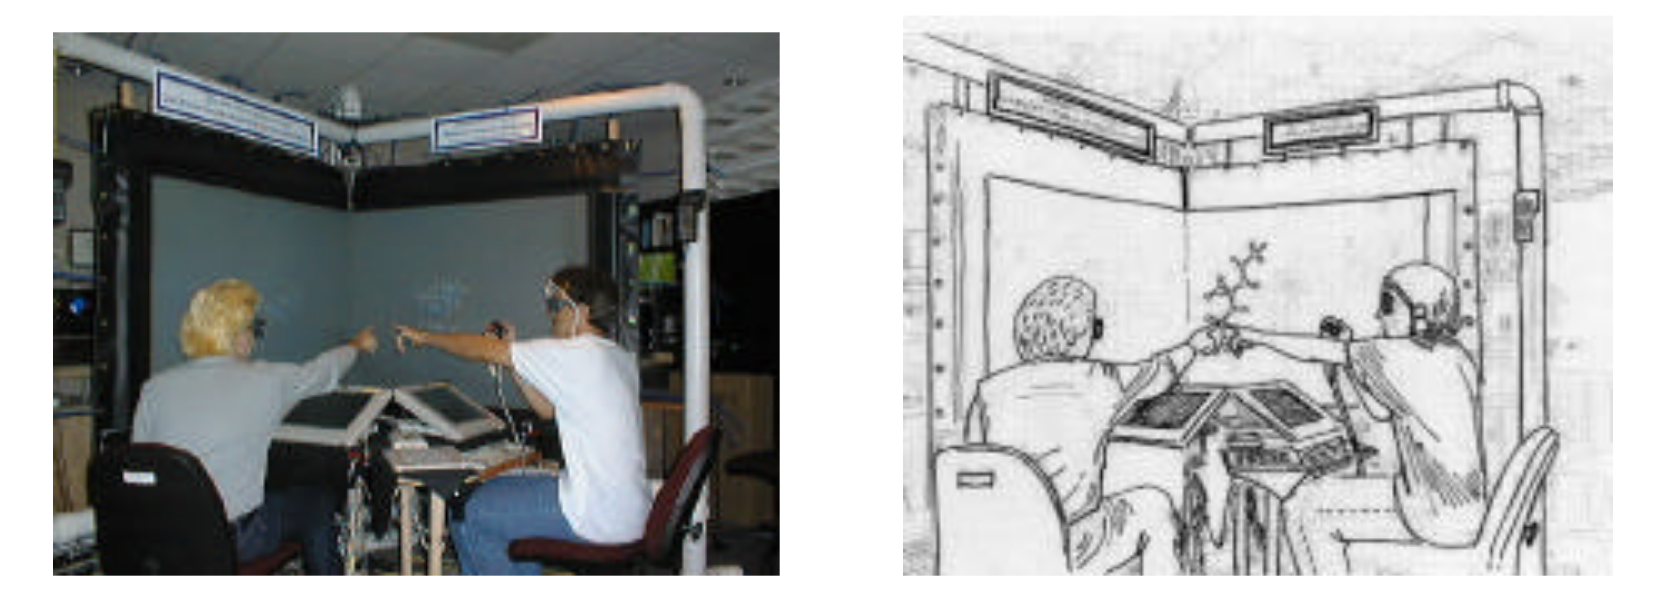
\includegraphics[width=\textwidth]{figures/ch1/steeredPIT}
		\caption[Dynamique moléculaire interactive en environnement virtuel]{Le logiciel de visualisation moléculaire VMD est utilisé avec les lunettes sétérographiques \emph{CrystalEyes} au sein du système \emph{Protein Interactive Theater} (PIT), qui permet l'immersion dans un environnement virtuel. Le PIT est par ailleurs couplé avec le module de simulation Sigma~\cite{mann2002sigma} pour permettre l'interaction avec la simulation. À gauche, une photo du PIT avec deux utilisateurs. À droite, un schéma de l'environnement virtuel tel qu'il est perçu par les utilisateurs. Crédit :~\cite{prins1999virtual}.}
		\label{fig:steeredPIT}
	\end{figure}
	
	Pour gérer des données aussi complexes que celles impliquées dans une simulation de dynamique moléculaire, l'immersion présente plusieurs avantages. Comme l'expliquent M.~Dreher \emph{et al.}~\cite{dreher2014exaviz}, le rendu stéréoscopique\footnotemark{} permet l'exploration de structures biologiques complexes qui sont intrinsèquement tridimensionnelles. De plus, la stéréoscopie avec suivi des mouvements de la tête permet à l'utilisateur de tourner autour d'objets 3D pour les examiner depuis différents points de vue, simplement en se déplaçant physiquement dans le système immersif, comme dans un contexte réel. Quand ce type de navigation n'est pas nécessaire, la stéréoscopie avec suivi de tête fournit à l'utilisateur la possibilité de se concentrer sur sa structure moléculaire et de l'étudier sous divers angles sans être distrait par les périphériques de navigation ou manipulation traditionnellement utilisés pour pallier le manque d'adaptation du rendu par rapport aux mouvements de tête.
	
	\footnotetext{La stéréoscopie vise à leurrer le système binoculaire humain, soit de façon active (lunettes à obturation ou \emph{shutter glasses}), soit de façon passive (lunettes polarisées ou autre filtrage spectral), en permettant la perception d'une image différente par œil.}
	
	\begin{figure}[!htbp]
		%\centering
		\begin{subfigure}[t]{0.40\textwidth}
			\centering
			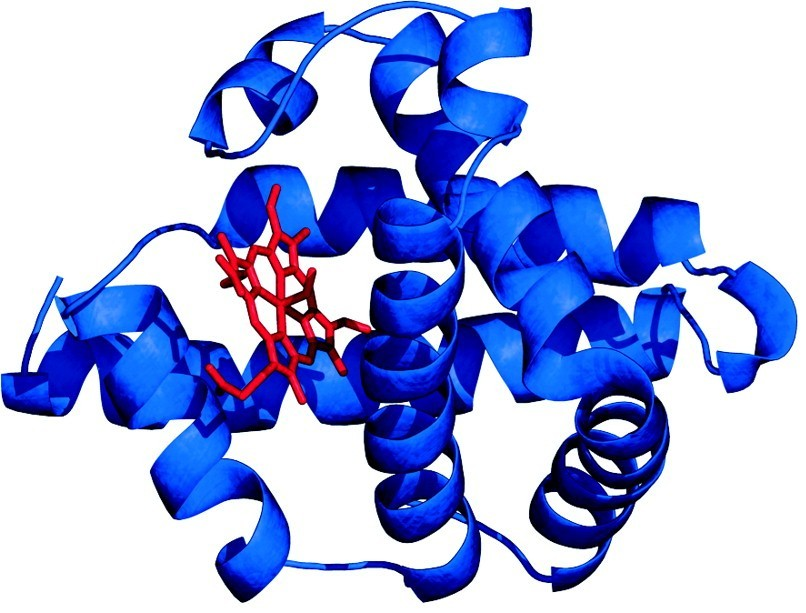
\includegraphics[width=\textwidth]{figures/ch1/myoglobin}
			\caption[Représentation hybride d'une protéine]{Molécule de myoglobine en  structures secondaires, avec son hème en \og tout atome \fg{} (en bâtons rouges). Les niveaux de densité et d'occultation sont donc compris entre ceux de ces deux modes de représentation. Crédit :~\cite{Ordway3441}.}
			\label{fig:myoglobin}
		\end{subfigure}
		~
		\begin{subfigure}[t]{0.58\textwidth}
			\centering
			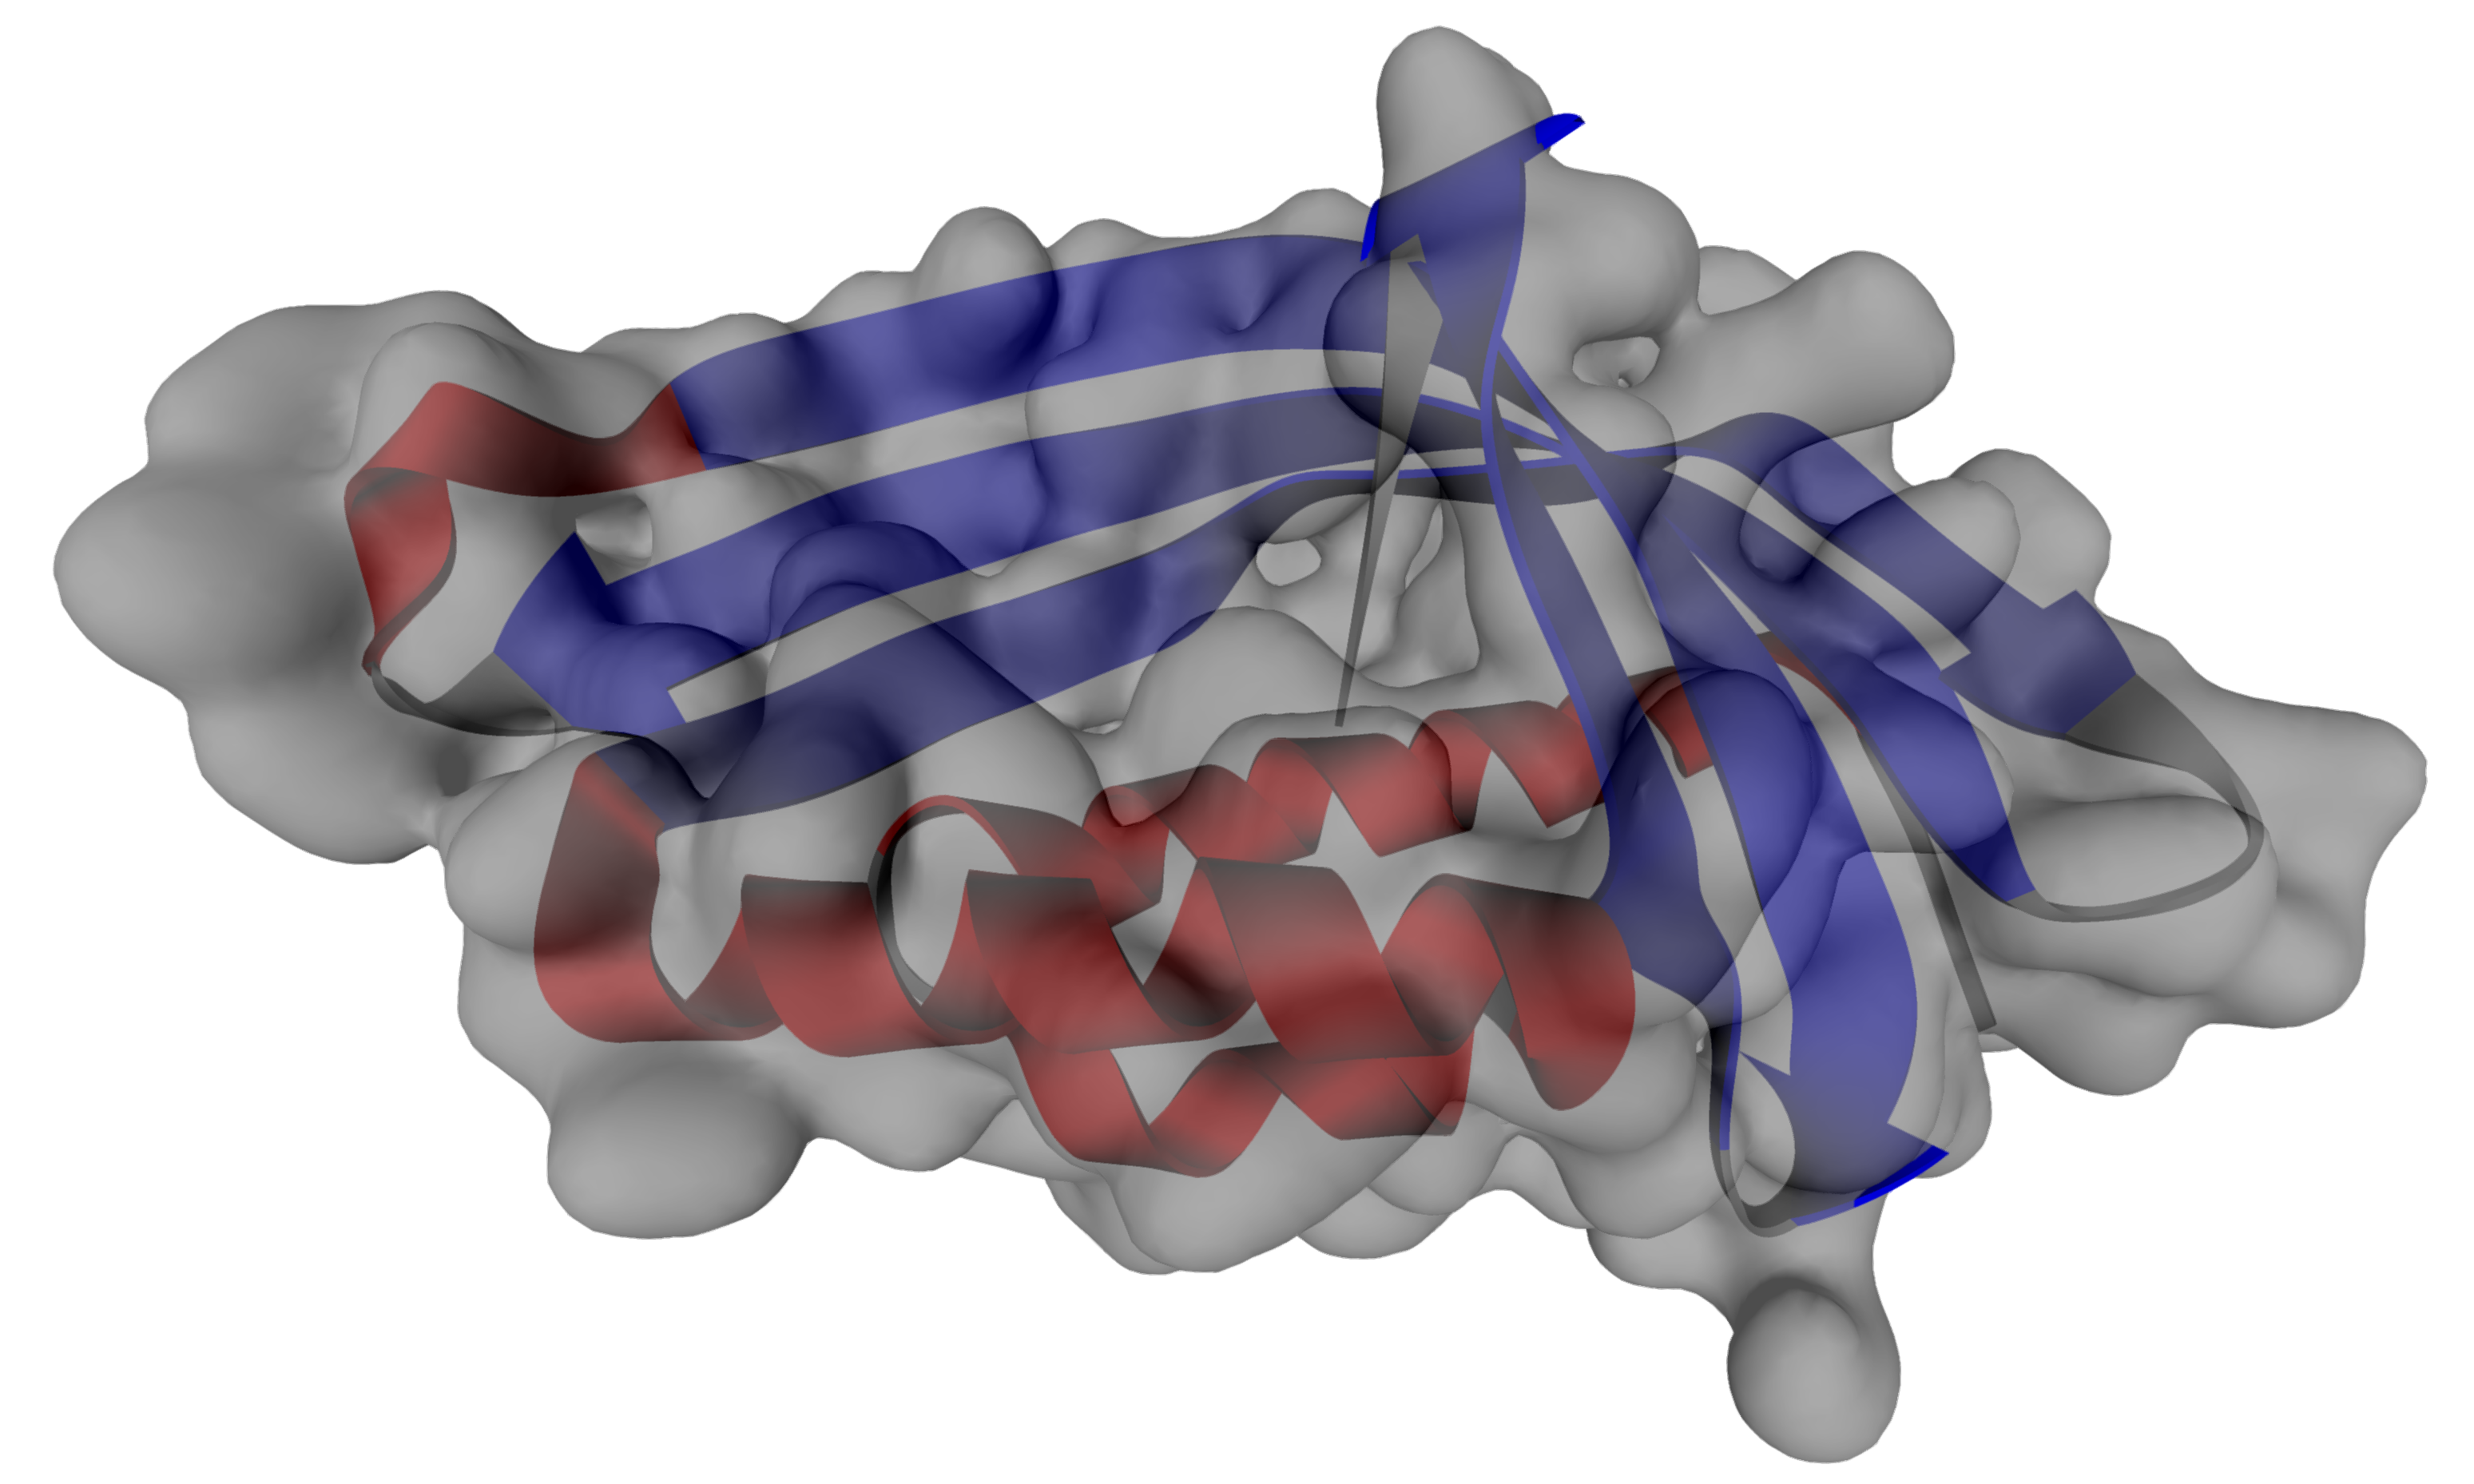
\includegraphics[width=\textwidth]{figures/ch1/transSS}
			\caption[Surface semi-transparente et structures secondaires]{Représentation hybride d'une protéine de chloroplaste, avec une isosurface de densité semi-transparente et les structures secondaires. On peut donc apprécier à la fois le volume occupé par la molécule et les aspérités de sa surface, mais aussi sa structure interne et certaines de ses propriétés physico-chimiques. Image générée avec \emph{UnityMol} à partir d'une structure de la \emph{Protein Data Bank}.}
			\label{fig:transSS}
		\end{subfigure}
		\label{fig:hybrid}
		\caption{Représentations hybrides de molécules.}
	\end{figure}	
	
	\begin{figure}[!htbp]
		\centering
		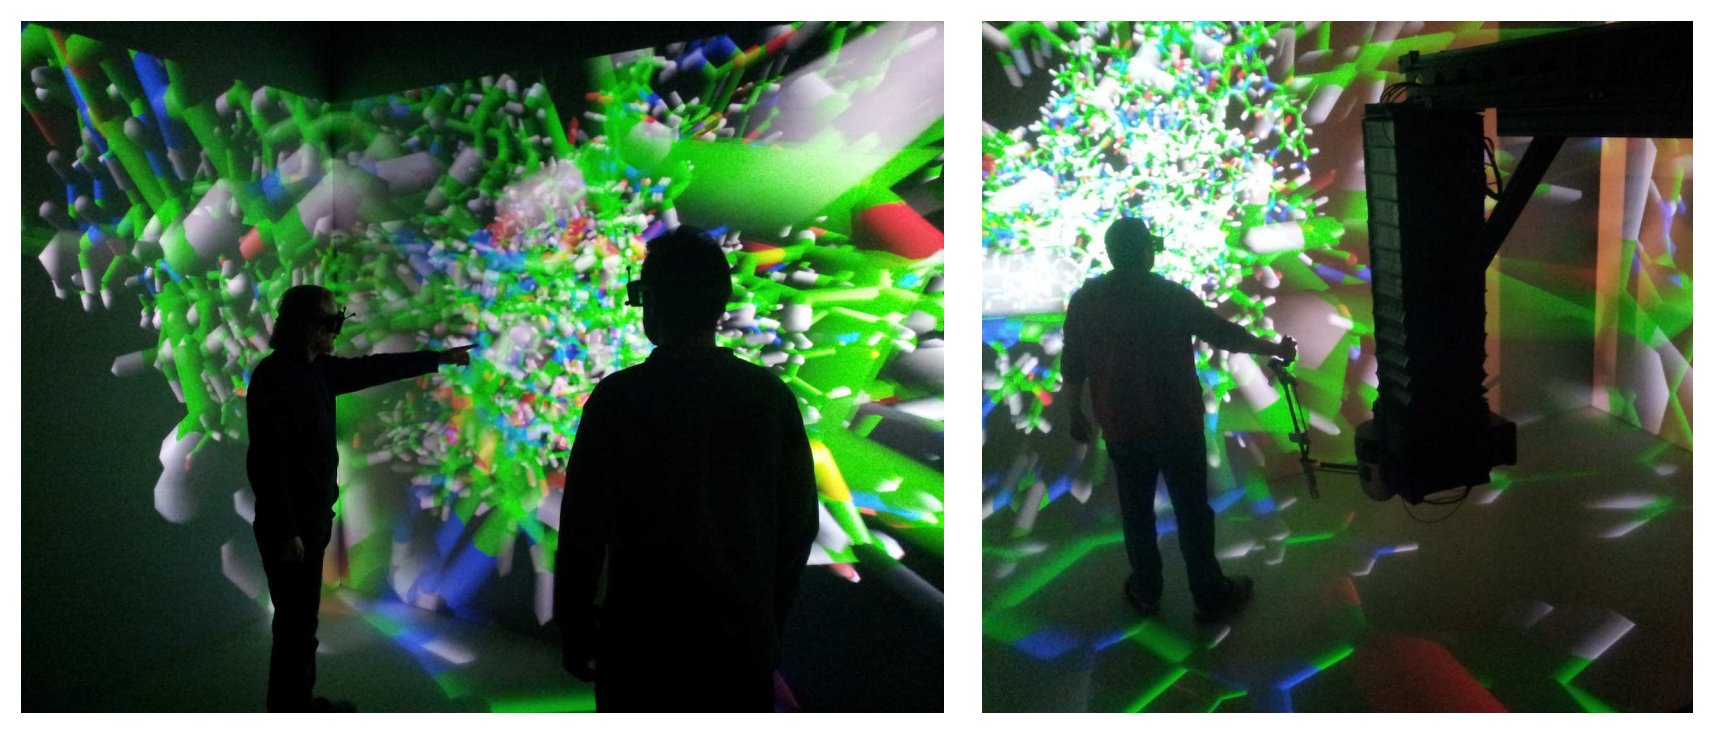
\includegraphics[width=0.9\textwidth]{figures/ch1/exaviz}
		\caption[IMD en environnement virtuel avec retour haptique, \emph{Exaviz}]{L'application \emph{Exaviz}. À gauche, deux utilisateurs dans le système EVE\footnotemark{} du groupe Venise, un CAVE multi-stéréoscopique ou deux utilisateurs peuvent avoir chacun une stéréoscopie propre à son point de vue dans la scène virtuelle. Ils peuvent ainsi collaborer et en particulier désigner avec exactitude et sans ambiguité pour l'autre utilisateur les objets virtuels. À droite, le SCALE ONE permet d'avoir des interactions avec retour d'effort dans la totalité du système EVE.. Crédits :~\cite{dreher2014exaviz, cazauxsysteme}.}
		\label{fig:exaviz}
	\end{figure}
	
	\footnotetext{Un CAVE permet l'immersion dans un environnement virtuel à l'aide de vidéo-projecteurs dirigés vers trois à six des murs d'une salle parallélépipédique. Ce nom est également une référence à l'allégorie de la caverne de Platon, dans laquelle le philosophe médite et expose ses vues sur la perception, la réalité et l'illusion. Le dispositif EVE de notre équipe, Venise, ajoute le support de la multistéréoscopie et du SCALE ONE. La première est une technologie projective couplant souvent des filtrages actif (lunettes à occultation) et passif (polarisation circulaire) afin de gérer différents points de vue dans la scène virtuelle. Le second est un bras haptique à 6 degrés de liberté sur un porteur translationnel à trois degrés de liberté, produit par la société Haption.
	 
	\url{http://www.limsi.fr/venise/EVEsystem}}
	
	Pour améliorer la perception des propriétés mécaniques des molécules étudiées, et des forces qui s'exercent sur elle, un retour haptique est possible au cours d'une simulation de dynamique moléculaire interactive~\cite{stone2001system}. Si l'haptique concerne le toucher et les phénomènes kinesthésiques, en pratique on utilise en IMD des bras haptiques, qui fonctionnent par retour de force.
	
	Ceux-ci peuvent être utilisés de diverses façons, notamment pour percevoir les \og collisions \fg{} entre le curseur et les objets de la scène, ou entre un objet sélectionné par l'utilisateur et un autre objet de la scène, pour permettre à l'utilisateur de percevoir les forces qui s'exercent entre les composantes de la molécule, ou encore pour guider la sélection, en appliquant une force au périphérique haptique dans la direction de la cible présumée de l'utilisateur. Le choix du mode d'utilisation d'un périphérique haptique dans une simulation d'IMD dépend de l'effet recherché.
	
	\subsection{Limites et défis actuels}
	L'interaction avec une simulation de dynamique moléculaire présente plusieurs difficultés majeures. Tout d'abord, le nombre de cibles potentielles est très élevé, avec au minimum plusieurs dizaines d'objets, jusqu'à plusieurs millions dans les cas les plus extrêmes. Ces cibles étant confinées dans un espace relativement petit, il en résulte de plus une densité élevée, voire très élevée (selon le mode de représentation). La figure~\ref{fig:exaviz} donne d'ailleurs une idée de cette densité ; cet exemple n'est pas le plus extrême, car la molécule visualisée n'est pas très grande et, surtout, le solvant n'est pas représenté.
	
	Il résulte naturellement de cette forte densité un niveau d'occultation très important. Cette occultation dépend également du mode de représentation utilisé. Le système moléculaire de la figure~\ref{fig:gluTrans}, du fait de l'utilisation de sphères de van der Waals, présente un degré d'occultation particulièrement important, et ce malgré le fait que le solvant n'est pas représenté.
	
	\begin{figure}[!htbp]
		\centering
		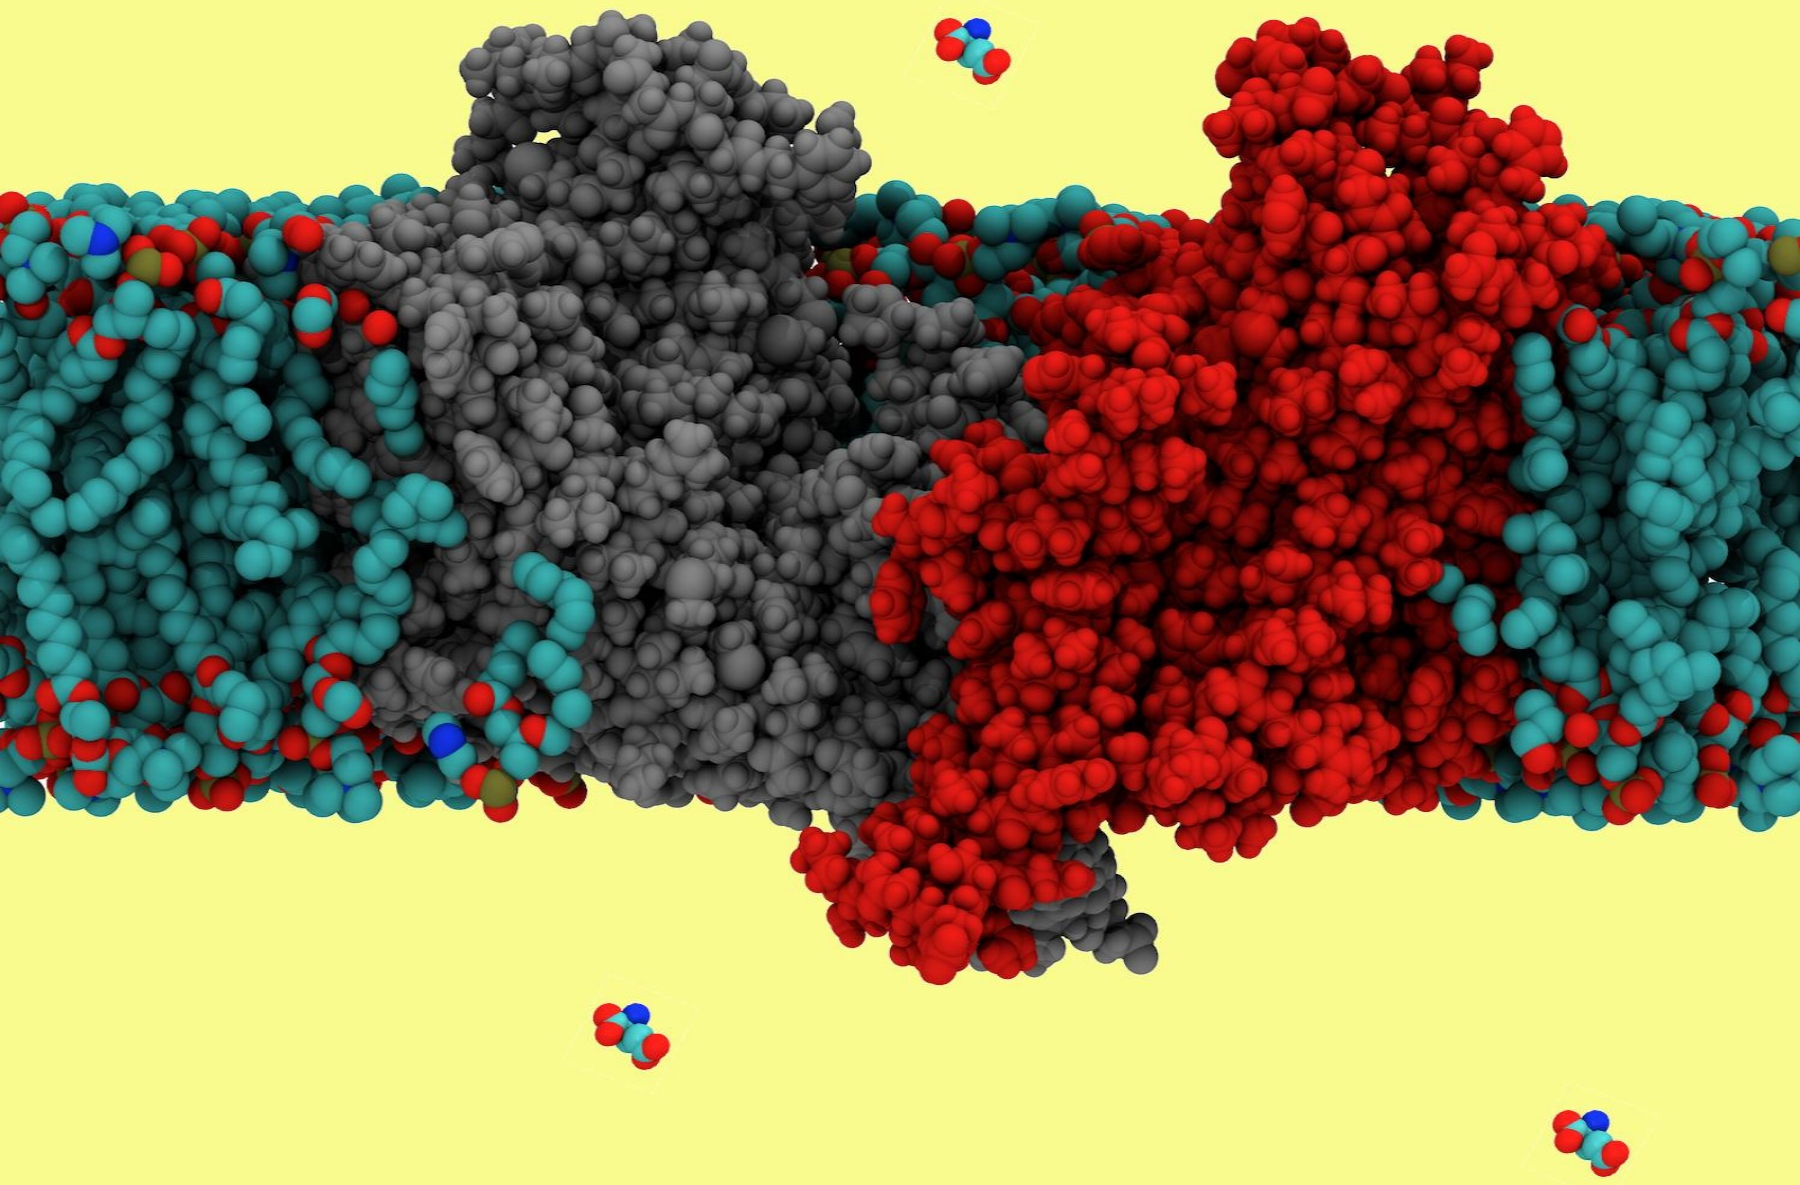
\includegraphics[width=0.6\textwidth]{figures/ch1/gluTrans}
		\caption[Transporteur de glutamate, très forte occultation]{Un transporteur de glutamate représenté en sphères de van der Waals, sans son solvant. C'est une protéine qui transporte le glutamate (forme ionisée de l'acide glutamique, c'est le neurotransmetteur excitateur le plus important du système nerveux central) à travers des membranes. Sur cette image issue d'une simulation de dynamique moléculaire, seule la surface de la molécule est visible, les atomes \og enfouis \fg{} sont entièrement occultés, alors qu'ils représentent la majeure partie de la molécule. Crédit : NVIDIA et Joshua Adelman\footnotemark.}
		\label{fig:gluTrans}
	\end{figure}
	
	\footnotetext{\url{https://blogs.nvidia.com/blog/2011/01/13/university-pittsburg-researcher-studies-molecular-dynamics-gpus}}
	
	Dans les simulations d'IMD, la vitesse des cibles peut être très élevée. Elle dépend en pratique de la vitesse de la simulation, donc de la taille du système simulé et des ressources de calcul disponibles, mais elle peut être supérieure à 10~\r{A}/s, sachant que le rayon d'un atome est d'environ 1~\r{A}.
	
	La périodicité des \og boîtes \fg{} de simulation introduit une difficulté particulière pour la sélection de cibles, puisqu'un objet peut quitter l'espace de sélection par un bord et le réintégrer par le bord opposé. Au-delà de l'effet de surprise, cela implique un changement brutal dans la distance entre le curseur et la cible, à moins que le curseur puisse se déplacer de la même manière.
	
	Quand il s'agit d'interagir avec un tel système, la vitesse d'une particule dans l'espace moteur dépend de la façon dont le système est représenté et du périphérique utilisé, mais elle devient rapidement problématique, \emph{a fortiori} quand la nature même du mouvement pose problème.
	
	En effet, les mouvements des atomes dans une simulation de dynamique moléculaire se caractérisent par leur irrégularité et, par conséquent, leur imprévisibilité. Selon la simulation et la façon dont elle est représentée, les atomes peuvent adopter un mouvement brownien ou plus proche de celui d'une mouche --- très vif, très saccadé et de fait imprévisible.
	
	En somme, les difficultés inhérentes à l'interaction avec les simulations de dynamique moléculaire incluent :
	
	\begin{itemize}
		\item la très forte densité de cibles,
		\item le haut degré d'occultation,
		\item la grande vitesse des cibles,
		\item la nature très imprévisible de leurs mouvements,
		\item la taille et la périodicité de l'environnement.
	\end{itemize}
	
	Ces facteurs combinés expliquent pourquoi les chercheurs en biologie structurale expriment le besoin de meilleurs modes d'interaction, et c'est la principale motivation des travaux présentés dans cette thèse.
	
	La biologie structurale n'est cependant pas le seul domaine caractérisé par un besoin d'interaction avec des cibles mobiles, loin s'en faut. Les sections suivantes vont passer en revue les principaux domaines ayant ce même besoin, mais avec des caractéristiques de mobilité très variées.
	
	%\section{Simulations de problèmes à N corps}
	
	\section{Contrôle de l'espace aérien}
 La figure~\ref{fig:airtraffic} représente un écran de contrôle du trafic aérien. Les trajectoires des avions sont (normalement) légèrement courbées ou rectilignes, ce qui les rend particulièrement prévisibles, et donc facilite considérablement la tâche de sélection, comme nous le verrons en détails plus loin. Cependant, selon le niveau de zoom et la quantité d'informations contextuelles affichées sur l'écran, le niveau d'occultation peut devenir très important. La vitesse des cibles dépend également du niveau de zoom, mais dans une relation inverse : plus l'échelle est grande, plus les mouvements des avions sont lents sur l'écran.
	
	\FloatBarrier \subsection{Applications civiles}
	
	\subsubsection{Avions}
	Un avion de ligne atterrit à environ 250~km/h et ne dépasse pas 1000~km/h en vol de croisière. Ses changements de direction sont très progressifs, généralement de l'ordre de deux degrés par seconde. Ils sont peu fréquents et habituellement prévisibles car les pilotes tâchent d'emprunter des couloirs aériens, ou des trajectoires d'approches imposées aux abords des aéroports. Les avions sont néanmoins nombreux, en particulier près des aéroports, et la grande quantité d'informations pertinentes associées à chaque vol peut requérir un affichage contextuel important, d'où une forte densité d'informations, et des niveaux d'occultation parfois élevés. La figure~\ref{fig:atlanta} en fournit un exemple.
	
	\begin{figure}[!htbp]
		\centering
		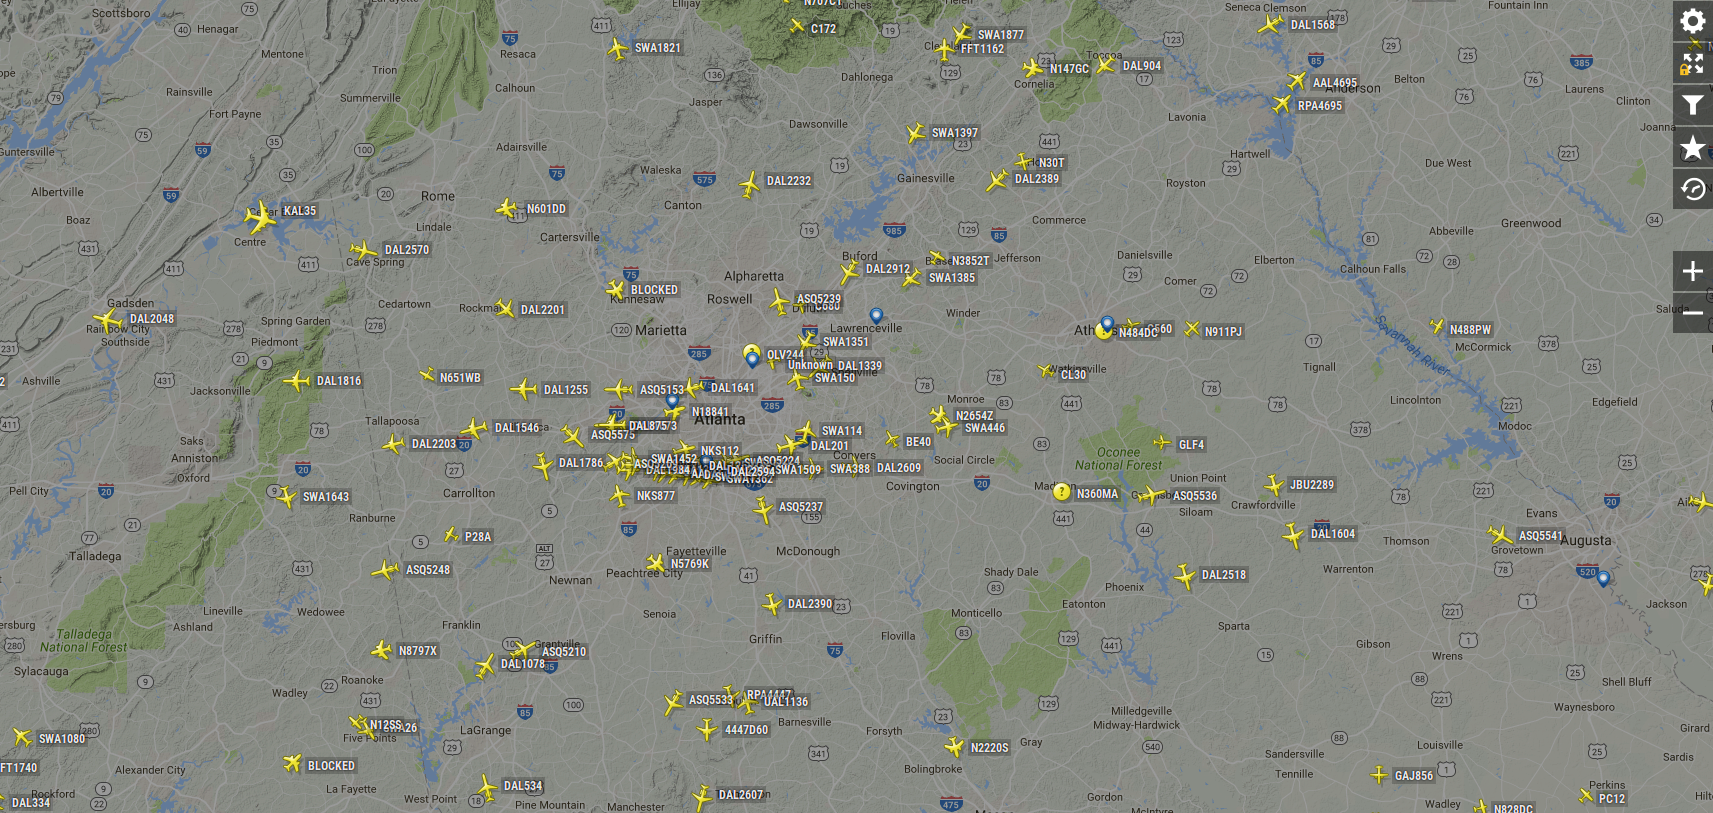
\includegraphics[width=\textwidth]{figures/ch1/atlanta}
		\caption[Trafic aérien, Atlanta]{Trafic aérien centré sur l'aéroport d'Atlanta, en Géorgie (États-Unis) un lundi matin vers 8~h~40. Chaque vol est représenté par un schéma de l'avion permettant d'indiquer son type, ainsi que par un identifiant de vol alphanumérique, de 5 à 7 caractères. Aucune information supplémentaire (origine ou destination du vol, trajectoire, altitude, pavillon de l'appareil, vitesse, horaires prévus, modèle exact de l'avion, carburant encore disponible, etc.) n'est affichée sur cette image, car aucun avion n'est sélectionné. Malgré tout, la densité d'informations est élevée et les appareils s'occultent mutuellement, surtout près de l'aéroport. Enfin, les vitesses apparentes (à l'écran) des avions demeurent faibles, sauf à un niveau de zoom élevé. Crédit : \emph{Flight Radar 24\footnotemark}.}
		\label{fig:atlanta}
	\end{figure}
	
	\footnotetext{\url{https://www.flightradar24.com}}
	
	Le Groupe \emph{Aéroports de Paris} (ADP) utilise un logiciel (encore en phase bêta) de visualisation et contrôle des aéroports permettant non seulement de surveiller les mouvements des avions en l'air et au sol, mais aussi de tous les véhicules au sol tels que les bus d'embarquement, les camions de ravitaillement, les véhicules de maintenance, de secours, etc. Ce logiciel est développé par une équipe du groupe Valtech\footnotemark{}, que nous avons rencontrée afin de mieux comprendre les besoins d'ADP, et les solutions actuellement mises en \oe{}uvre.
	
	\footnotetext{\url{https://www.valtech.fr}}
	
	La nature de la tâche implique une quantité de données contextuelles très importante, puisque le logiciel permet d'afficher notamment le statut de chaque avion, ses codes d'identification, sa destination ou son origine, son retard éventuel, le statut de ses bagages ou de ses passagers, la liste des passagers en question, les pistes et emplacements de stationnement qui lui sont alloués ou disponibles, sa compagnie, son type, etc. La figure~\ref{fig:adp} fournit un exemple modéré de la quantité d'informations potentiellement affichées.
	
	\begin{figure}[!htbp]
		\centering
		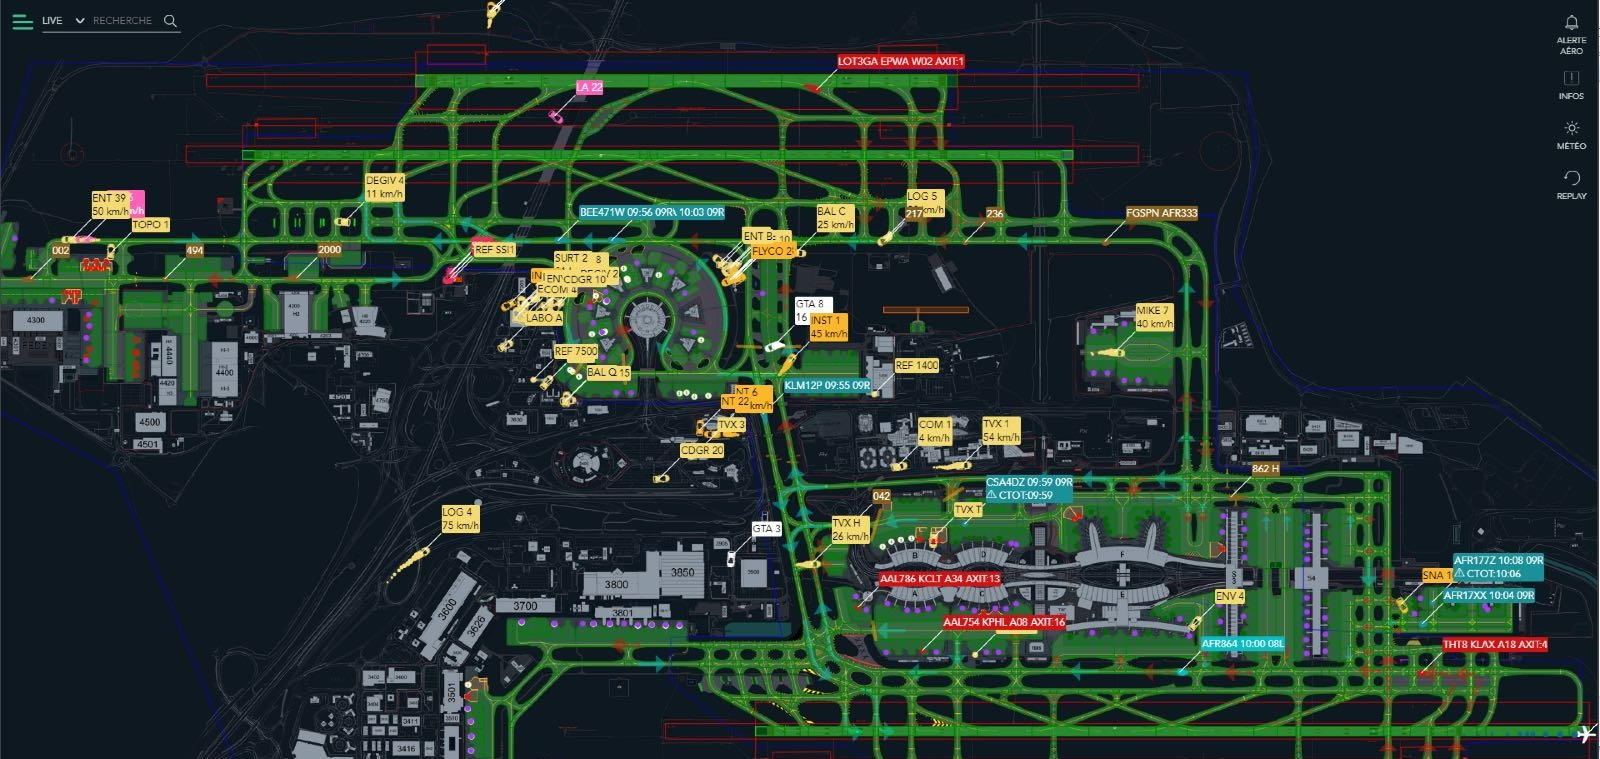
\includegraphics[width=\textwidth]{figures/ch1/adp}
		\caption[ADP -- Roissy]{Exemple de visualisation de l'aéroport de Paris--Charles-de-Gaulle avec le logiciel utilisé par le groupe ADP. Seuls les véhicules terrestres sont affichés ici, et les informations contextuelles sont limitées ; pourtant, la densité de cibles est importante, de même que le niveau d'occultation visuelle. Crédit : Valtech.}
		\label{fig:adp}
	\end{figure}
	
	Les informations mises à disposition de l'utilisateur ne se limitent pas aux données brutes sur l'aéroport, les avions et autres véhicules, mais incluent des flux vidéo, capturés par des centaines de caméras réparties sur tout l'aéroport. À tout moment, l'utilisateur peut choisir d'ajouter à sa vue un ou plusieurs flux vidéo (par exemple en sélectionnant toutes les caméras filmant un point particulier). Le logiciel utilisé par le groupe ADP, qui fournit des capacités d'action telles que l'ouverture ou la fermeture en temps réel d'un tronçon de piste, est particulièrement utile pour rejouer des situations, et en particulier des incidents --- qui sont le plus souvent mineurs. Dans ce contexte, les caractéristiques réelles de mouvement des avions sont secondaires par rapport aux caractéristiques perçues lorsque les incidents sont rejoués, généralement en accéléré. Dans ce cas, les cibles déjà nombreuses, diverses et mobiles, deviennent plus rapides, selon le facteur d'accélération --- qui peut être très élevé.
	
	Cette application a en plus vocation à permettre à son utilisateur d'alerter les autorités en cas de détection d'une personne présentant un risque de sécurité, notamment lié au terrorisme. Il sera évidemment nécessaire de pouvoir effectuer cette opéation dans les plus brefs délais, ce qui implique une forte contrainte sur la performance de l'interface, notamment pour la sélection de l'élément jugé menaçant.
	
	Enfin, un des objectifs de ce logiciel est de pouvoir être utilisé depuis un périphérique mobile, par exemple une tablette embarquée dans un véhicule de maintenance ou d'urgence. De fait, les informations doivent pouvoir être affichées sur un écran d'environ 10 pouces. Dans ces conditions, le problème de surcharge visuelle est encore plus prégnant et potentiellement gênant pour la sélection, du moins si la quantité d'informations affichées demeure la même. Une technique d'assistance à la sélection n'en est que plus souhaitable.

	\subsubsection{Hélicoptères}
	Comme les aéronefs à voilure fixe, les hélicoptères s'insèrent dans la circulation aérienne et il est nécessaire de les surveiller. Leurs caractéristiques de vol sont néanmoins quelque peu différentes de celles des avions, puisqu'ils peuvent faire demi-tour en environ quatre secondes, voire moins. Ils sont beaucoup plus lents que les avions : les modèles civils dépassent rarement les 300~km/h. La fréquence des changements de direction dépend considérablement de la mission, elle peut être très faible pour un simple transport d'un point A vers un point B, auquel cas la trajectoire de l'hélicoptère va tendre vers la ligne droite, plus importante dans le cadre d'une mission de secours en montagne, et plus importante encore pour un hélicoptère de police fournissant une assistance aérienne pendant une course-poursuite, ou pour un hélicoptère utilisé pour filmer un événement sportif, un documentaire animalier, une manifestation, des émeutes, etc.
	
	\FloatBarrier \subsection{Sécurité et défense (surveillance de l'espace aérien)}
	Les aéronefs militaires présentent des caractéristiques beaucoup plus variables, dans des intervalles nettement plus grands. C'est notamment dû à leur diversité, puisque l'on trouve des avions de tailles et usages divers, des drones de quelques grammes comme de plusieurs tonnes, des hélicoptères, des missiles, etc.
	
	\subsubsection{Avions de combat}
	La vitesse d'un avion de combat, par exemple, peut atteindre 3000~km/h\footnotemark. Il est beaucoup plus difficile d'obtenir des données chiffrées sur la manœuvrabilité de tels engins, mais il est du moins clair qu'un avion de combat moderne peut changer de direction beaucoup plus brutalement qu'un avion de ligne, et certaines sources non officielles font état de capacités de l'ordre de 35\textdegree{}/s pour les meilleurs\footnotemark. Des données officielles font état de 12,9\textdegree{}/s \emph{soutenus} pour le Leonardo DRS T-100, qui n'est pourtant qu'un avion d'entraînement\footnotemark.
	
	\addtocounter{footnote}{-2}
	\footnotetext{\url{http://www.migavia.ru/index.php/en/production/mig-31e-fighter?limit=1&start=2}}
	\addtocounter{footnote}{1}
	\footnotetext{\url{https://defenseissues.net/2014/01/11/comparing-modern-western-fighters/}}
	\addtocounter{footnote}{1}
	\footnotetext{Pour un taux de changement de direction \emph{soutenu} donné, le taux instantané est toujours supérieur.
	\url{http://www.leonardodrs.com/media/5278/007152_01_drs_t100_datasheet_v2.pdf}}
	
	La fréquence maximale à laquelle un avion peut changer de direction est également difficile à connaître avec certitude, d'autant qu'elle dépend de la façon dont on définit un changement de direction, mais une simple observation d'une démonstration en vol permet d'estimer que cette valeur est, grossièrement, de l'ordre d'un changement par seconde environ\footnotemark. Indépendamment des capacités techniques des avions militaires, leurs missions peuvent précisément imposer la recherche de l'imprévisibilité (par exemple pour éviter les tirs ennemis)~\cite{shaw1985fighter} ce qui n'est généralement pas le cas dans le civil.
	
	\footnotetext{Démonstration en vol : \url{https://www.youtube.com/watch?v=vo0ZN2_O29M}}
	
	\begin{figure}[!htbp]
		\centering
		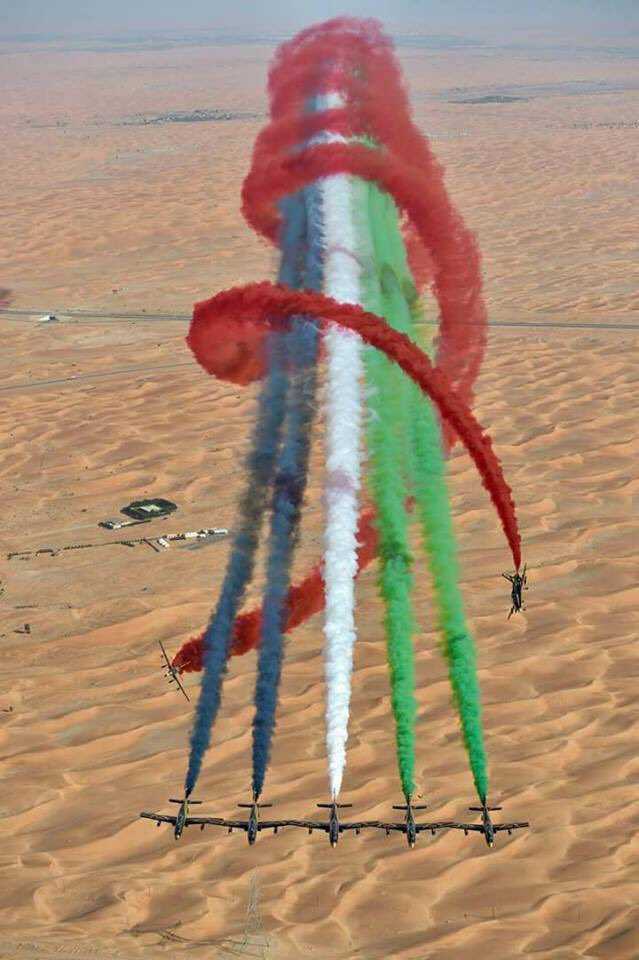
\includegraphics[width=\textwidth]{figures/ch1/AlFursan}
		\caption[La patrouille acrobatique \emph{Al Fursan}]{La patrouille acrobatique émiratie \emph{Al Fursan}, avec ses trajectoires entremêlées mises en évidence par des traînées de fumée colorées. Des avions militaires peuvent avoir des trajectoires à la fois complexes, très proches les unes des autres, et parcourues à grande vitesse. Crédit : The National UAE\footnotemark.}
		\label{fig:alfursan}
	\end{figure}
	
	\footnotetext{\url{http://www.thenational.ae}}
	
	Il convient de noter que les avions de combat eux-mêmes ont des besoins similaires en matière de sélection de cibles mobiles, puisqu'ils ont, comme les stations au sol, pour rôle de contrôler l'espace aérien. Ils ont de plus la charge de mener des opérations de reconnaissance ou de bombardement de cibles au sol qui, si elles sont statiques, sont bien mobiles dans le référentiel de l'avion en vol, \emph{a fortiori} si elles sont filmées par des caméras mobiles. Par ailleurs, les cibles affichées sur les ordinateurs de bord des avions sont accompagnées de diverses informations tactiques qui augmentent fortement la densité d'informations, et potentiellement le niveau d'occultation, comme l'illustre la figure~\ref{fig:sitac}.
	
	\begin{figure}[!htbp]
		\centering
		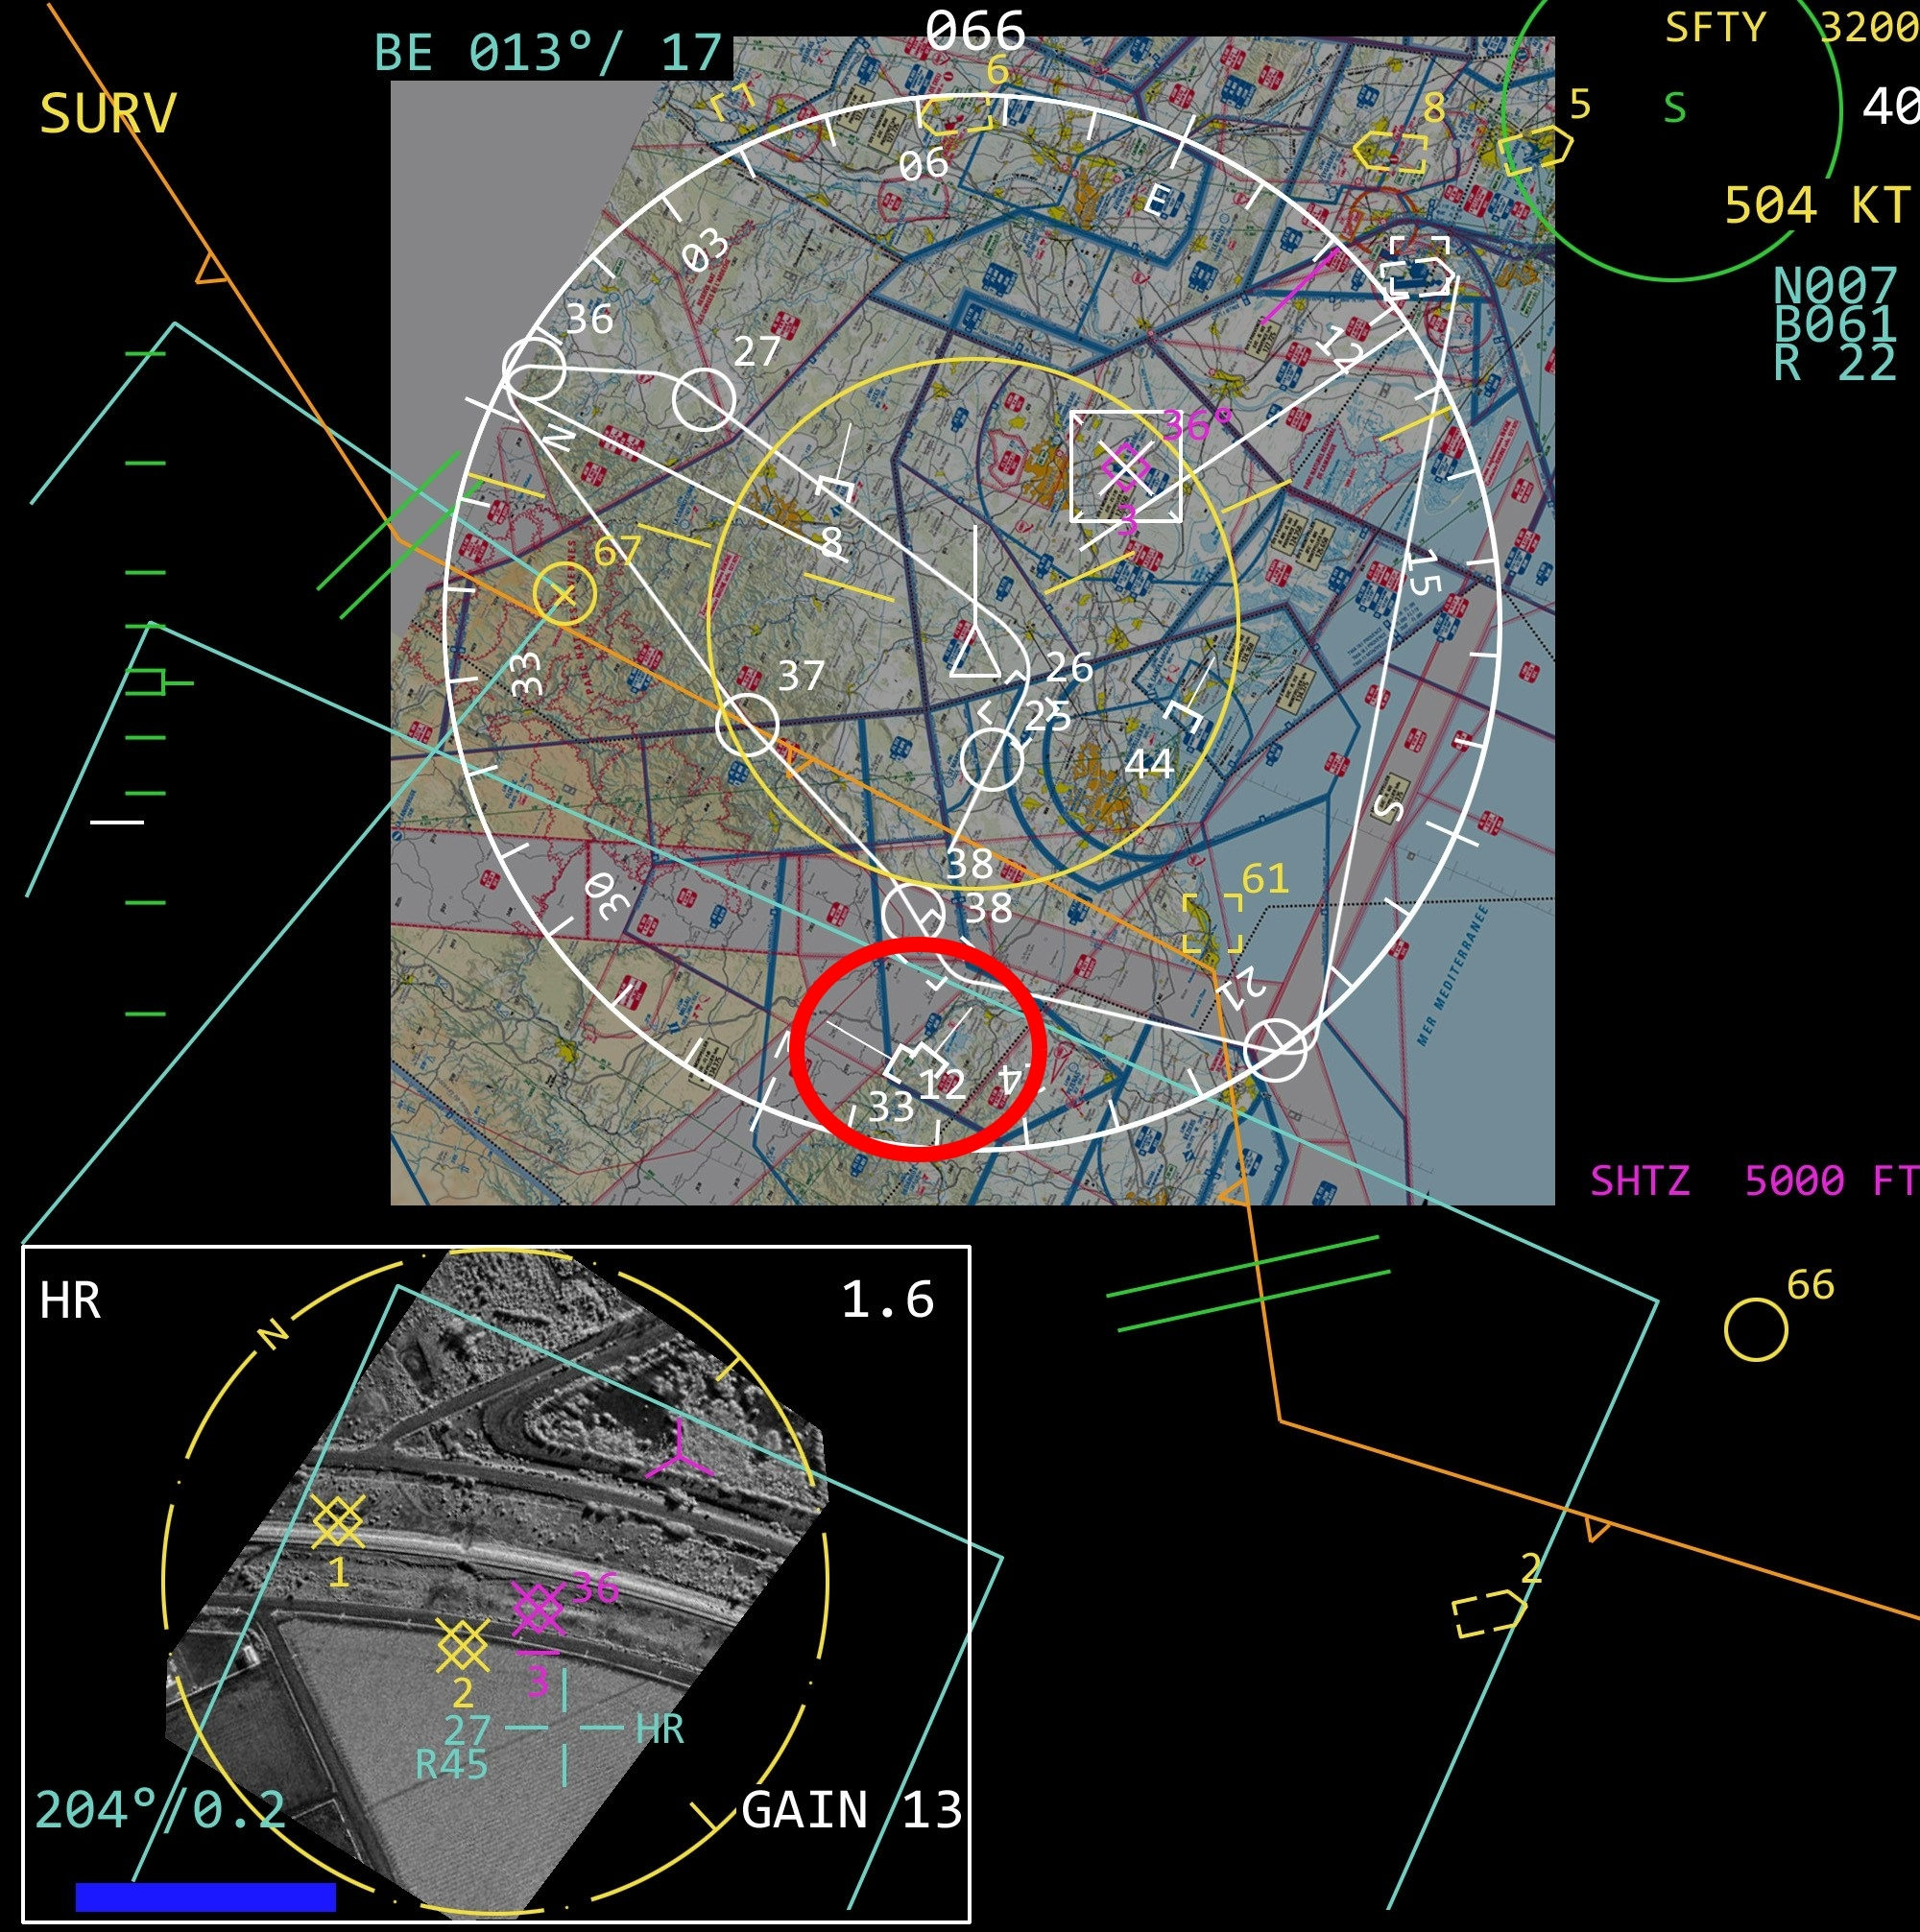
\includegraphics[width=\textwidth]{figures/ch1/sitac}
		\caption[Situation tactique vue d'un \emph{Rafale}]{Cette image représente une situation tactique telle qu'affichée sur un écran dit \og visualisation tête moyenne \fg{} dans un \emph{Rafale} de Dassault Aviation. Sur cette image très \og chargée \fg{} seuls deux petits symboles, que nous avons ici entourés en rouge, représentent des avions ennemis. Au-delà de la carte de fond, les autres symboles représentent diverses informations tactiques importantes : l'avion lui-même bien sûr, sa direction, un compas de route, l'altitude maximale des obstacles terrestres, l'échelle, la vitesse de l'avion, le plan de vol, la ligne de front, un zoom, etc. Par conséquent, même avec un très petit nombre de cibles potentielles, l'affichage est complexe, dense, et potentiellement gênant pour la sélection. Crédit : Portail Aviation\footnotemark.}
		\label{fig:sitac}
	\end{figure}
	
	\footnotetext{\url{http://www.portail-aviation.com/2015/07/exclusif-a-la-decouverte-de-la-situation-tactique-du-rafale-sitac.html}}
	
	Un ancien instructeur de vol de la \emph{United States Air Force}\footnotemark{} sur McDonnell Douglas F-15C \emph{Eagle} nous a expliqué par ailleurs que lors d'un engagement armé, il est courant qu'un groupe de chasseurs vole délibérément en formation très serrée, plus serrée que la largeur du faisceau radar des chasseurs ennemis. Il est de fait difficile pour ces derniers de savoir à combien d'adversaires ils ont affaire, du moins jusqu'à la séparation --- généralement très abrupte --- de la formation serrée. L'objectif est de permettre à au moins un chasseur de se mettre en position favorable sans être vu.
	
	\footnotetext{Ou USAF, la force aérienne des États-Unis d'Amérique.}
	
	Par conséquent, l'on passe d'une seule cible (apparente) à plusieurs cibles d'abord très rapprochées, mais souvent rapidement divergentes. Parfois, les pilotes plongent vers le sol pour utiliser les retours radar du relief afin de masquer le leur ; ajoutons que c'est d'autant plus efficace que l'aéronef est furtif, et qu'il peut donc apparaître et disparaître des écrans radar à tout moment. Ce point est d'autant plus important que les technologies furtives se répandent progressivement et les aéronefs furtifs sont de plus en plus courants. Parmi les plus connus, on peut citer le Northrop Grumman B-2 \emph{Spirit}, ainsi que le F-35 \emph{Lightning II} produit par Lockheed Martin.	
	
	\newcommand{\subImgAircraftW}{0.74\textwidth}
	\begin{figure}[!htbp]
		\centering
		\begin{subfigure}[t]{\subImgAircraftW}
			\centering
			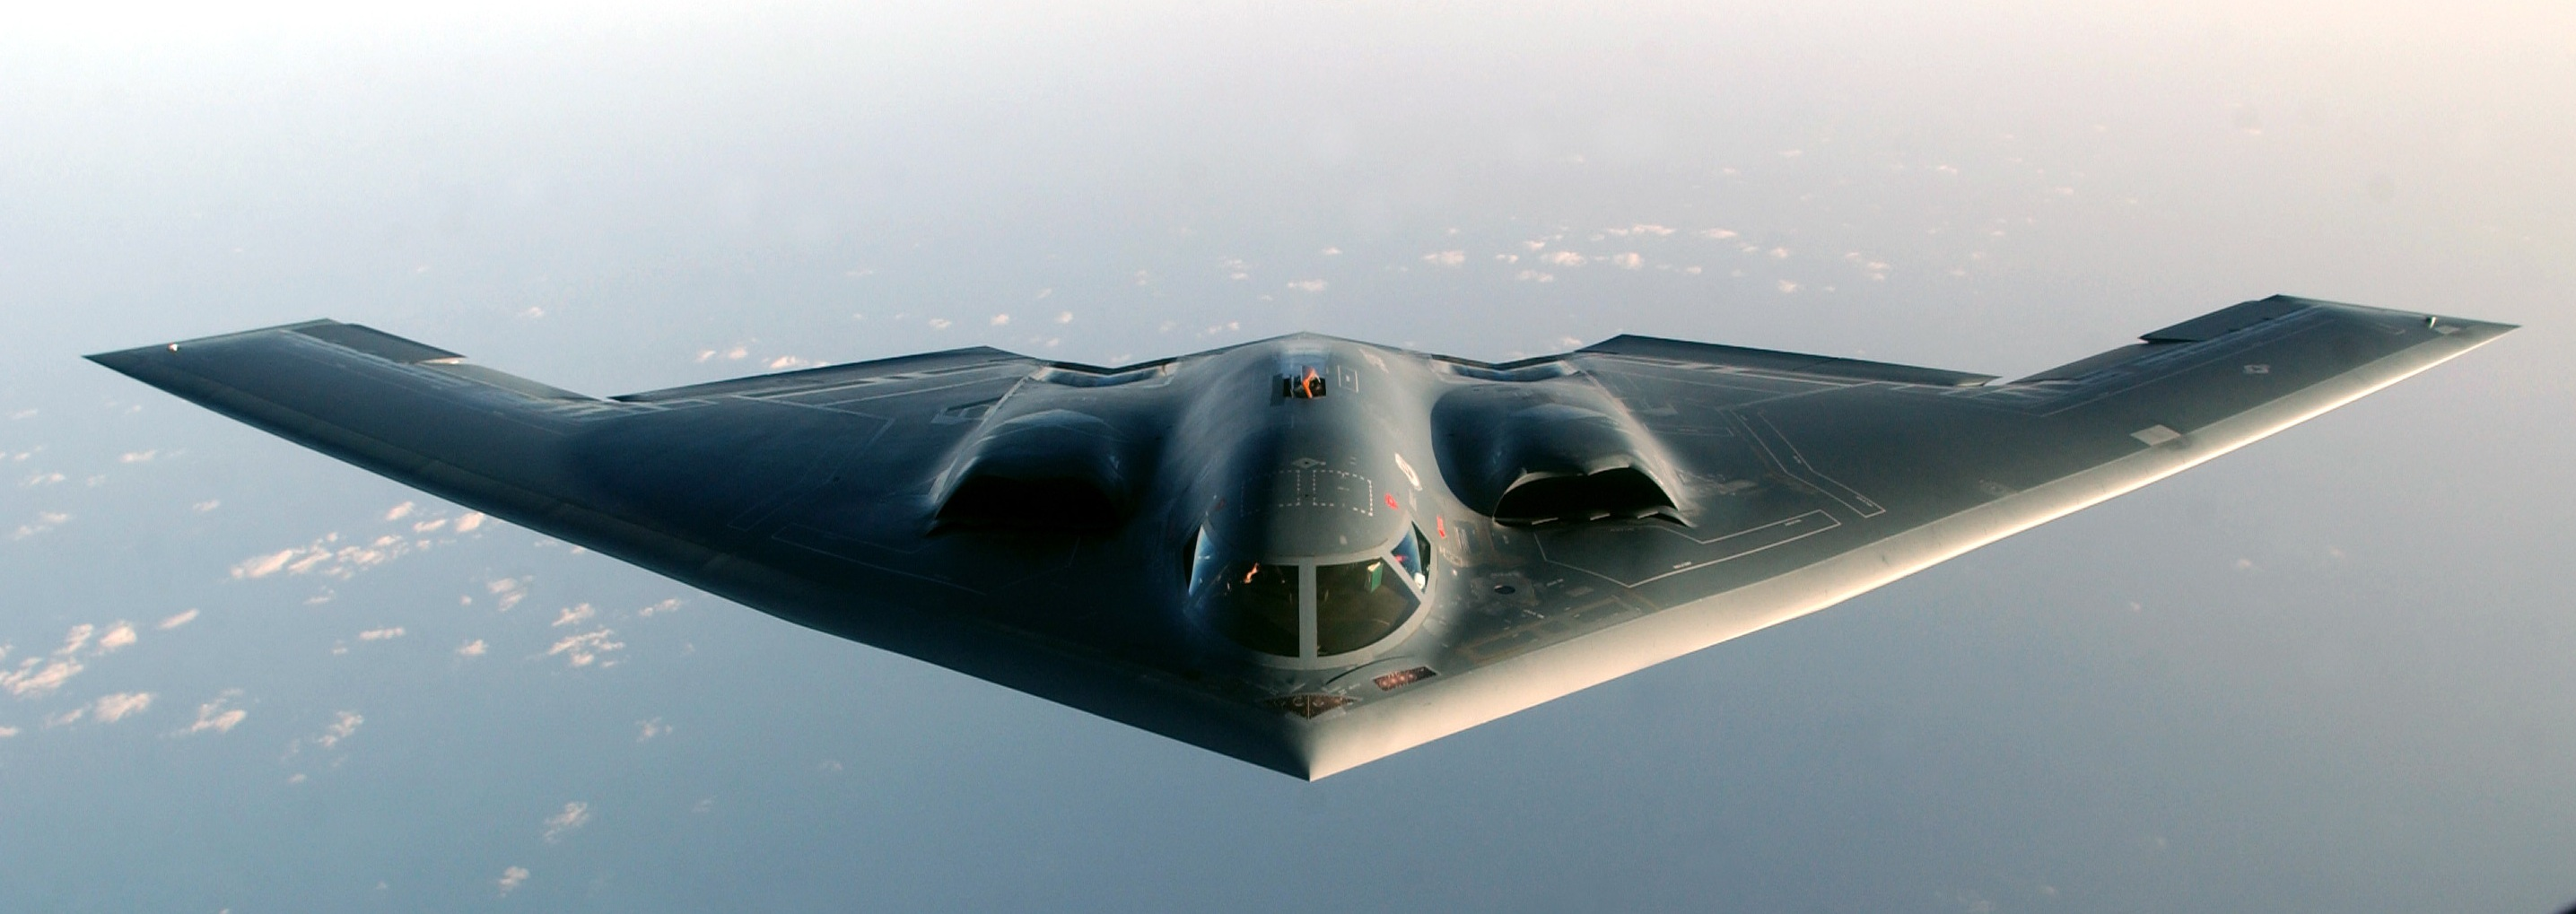
\includegraphics[width=\textwidth]{figures/ch1/B2}
			\caption[Northrop Grumman B-2 \emph{Spirit}, un bombardier stratégique furtif]{Le Northrop Grumman B-2 \emph{Spirit}, un bombardier stratégique furtif de l'USAF. Sa forme d'aile volante, son alignement de plans jamais perpendiculaires à son axe longitudinal, le placement de ses moteurs sur son dos, enfouis dans le fuselage, l'utilisation de matériaux composites absorbants, etc., contribuent à réduire la signature de cet appareil dans plusieurs bandes électromagnétiques. Crédit : \emph{Wired}.}
			\label{fig:B2}
		\end{subfigure}
		~
		\begin{subfigure}[t]{\subImgAircraftW}
			\centering
			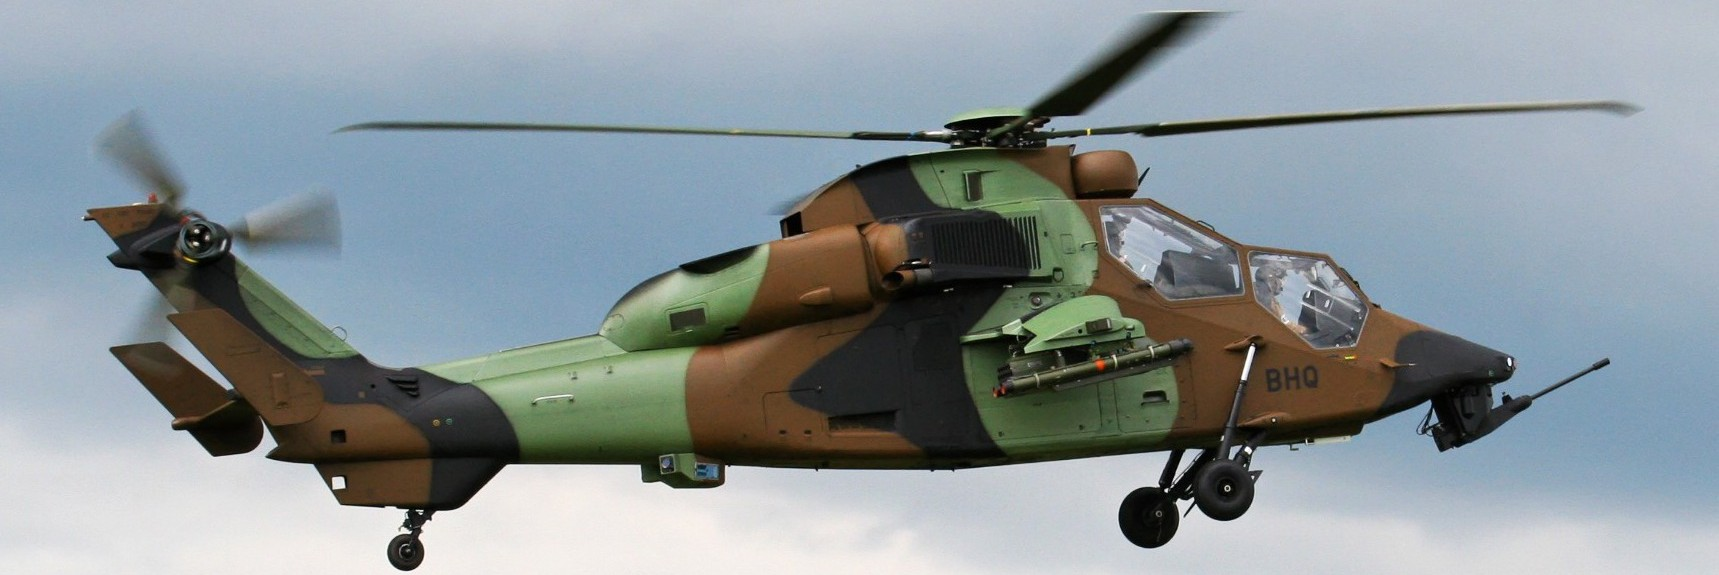
\includegraphics[width=\textwidth]{figures/ch1/tigre}
			\caption[Hélicoptère d'attaque \emph{Tigre}]{L'hélicoptère d'attaque \emph{Tigre} conçu et fabriqué par Airbus Helicopters. Cet aéronef est capable de voler jusqu'à 370~km/h en piqué, et il est assez manœuvrable pour changer de direction de vol très rapidement (sans nécessairement changer l'orientation de l'engin, par exemple en volant latéralement), voler à très basse altitude en suivant le terrain, effectuer des tonneaux, \emph{loopings}, etc., notamment grâce à sa capacité de tolérer des accélérations allant jusqu'à 4g~\cite{tigre}. Crédit : \emph{Wikimedia}}
			\label{fig:tigre}
		\end{subfigure}
		~
		\begin{subfigure}[t]{\subImgAircraftW}
			\centering
			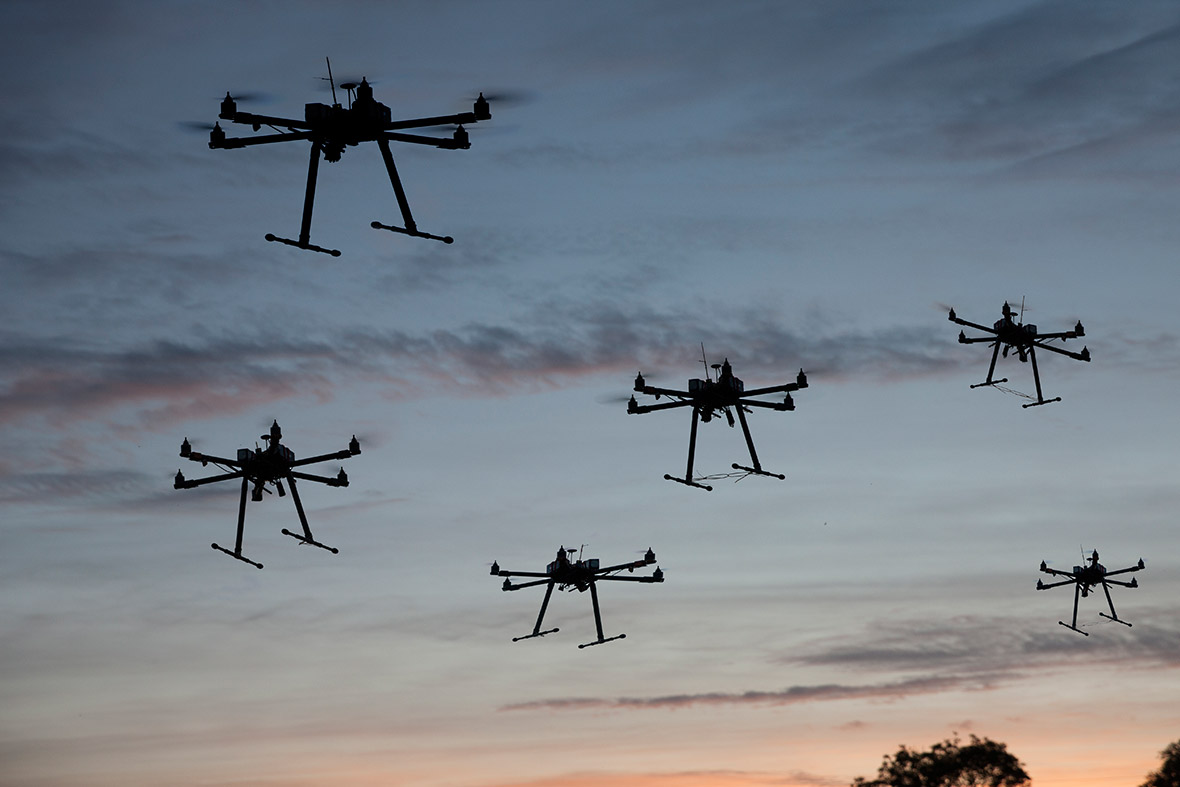
\includegraphics[width=\textwidth]{figures/ch1/swarm}
			\caption[Petit essaim de drones aériens]{Petit essaim de drones aériens. Ces engins simples et peu coûteux peuvent être produits et utilisés en très grand nombre. Ils sont souvent capables d'évoluer en formation serrée, donc de constituer un ensemble de cibles très dense. Crédit : \emph{International Business Times}.}
			\label{fig:swarm}
		\end{subfigure}
		\caption{Aéronefs militaires.}
		\label{fig:coolAircraft}
	\end{figure}
	
	À ces appareils de l'USAF s'ajoutent aujourd'hui le Chengdu J-20 chinois, ainsi qu'un nombre d'avions encore en développement : le Sukhoi Su-57 russe, le B-21 \emph{Raider} de Northrop Grumman, le drone franco-britannique FCAS/SCAF, et bien d'autres.
	
	Le combat aérien est une application qui peut mêler une très forte densité de cibles (avec un taux d'occultation considérable), parfois évanescentes, à des mouvements rapides et délibérément imprévisibles. De plus, détecter et sélectionner les cibles aussi rapidement que possible revêt une importance littéralement capitale, puisque les pilotes jouent leur vie, sans parler des enjeux stratégiques et humains spécifiques au conflit en question.
	
	%If you have sneaky guys like me, at long range we’ll fly in ‘res cell’ which means we’ll be so close to each other we’re closer than the width of the radar beam at that range. That makes it difficult to know exactly how many people are in an attack or air defense package. Then, at some pre-designated range, we’ll do very abrupt maneuvers and split while guys who are locked or not locked (spiked or not spiked) will do different things to optimize our chances of getting at least one good guy untargeted and unseen to a merge.

    %When we first started using AIM-120’s in the F-15C, we would often have a 2-ship of AMRAAM shooters against a 4-ship of AIM-7 shooters. If I was leading a 4-ship, I would bring us in wide apart to make it easy for the other 2-ship to find/sort/shoot us. Then we’d meld back into one small formation. Then I’d do a 90 degree turn and dive to the deck with chaff while the other 3 split wide and all changed altitudes but ended up doing 180 turns away at a range the missiles could be defeated kinematically.

    %Then using GCI (ground-controlled interception), I would E & E at very low altitude to get past and underneath them and then come up from behind and not use my radar until one guy was shot with a no-lock AIM-9 and then I would lock to let the other guy know he was about to ‘die’ from my AIM-7.

    %In Alaska, we had the kind of contrails that would show with power up but would go away with power in IDLE. In most places, if you have cons, you’ll also have cons in low power.

    %So we climb a 4-ship through the cons and then above so the bad guys can see 4 contrails. Then a sneaky guy . . . me . . . would descend in a 90 degree turn in IDLE with chaff and descend to low altitude with NO contrail so the opponents think we are all above the cons leaving me free to maneuver behind them on the deck. It was a very effective tactics at times.
	
	\subsubsection{Hélicoptères de combat}
	De même, les hélicoptères militaires sont plus agiles que leurs homologues civils, sans qu'il soit aisé de quantifier cette différence. Comme pour les avions, leur comportement est susceptible de varier considérablement selon la mission. Ils sont ausssi légèrement plus rapides, de quelques dizaines de km/h, notamment en piqué. Comme pour les avions, leurs missions impliquent souvent des trajectoires moins prévisibles, d'autant qu'ils cherchent souvent à se camoufler (visuellement et pour les radars) en volant le plus bas possible, ce qui implique de contourner les éléments de relief. L'hélicoptère Eurocoptère \emph{Tigre} représenté sur la figure~\ref{fig:tigre} est un exemple d'appareil rapide, compact et très manœuvrable.
	
	Du fait de leur capacité à voler à très basse altitude, et souvent entre les éléments de reliefs (par exemple dans des vallées) les hélicoptères ont tendance à n'apparaître que brièvement sur les écrans radar. De fait, s'ils ne sont pas nécessairement des cibles d'un comportement extrêmement vif ou imprévisible, il peut n'être possible de les sélectionner que pendant de très courts laps de temps. Leur sélection peut par conséquent être particulièrement difficile et nécessite une assistance efficace.
	
	Pendant la guerre du Golfe, par exemple, un McDonnell Douglas F-15E \emph{Strike Eagle} se trouva dans l'impossibilité de verrouiller son radar sur un hélicoptère Mil Mi-24 \emph{Hind} irakien pour l'abattre à l'aide d'un missile, du fait de la proximité du Mi-24 au sol et de la vivacité de ses mouvements. L'officier des systèmes d'armes du F-15E dut basculer vers la nacelle de désignation laser pour \og marquer \fg{} l'hélicoptère afin de le détruire à l'aide d'une bombe~\cite{craig2007debrief}. L'officier en question ne précise pas si cette désignation fut difficile, attendu qu'il l'effectua avec un outil conçu pour cibler des objets statiques ou, à la rigueur, lents.
	
	\footnotetext{\url{https://theaviationist.com/2016/02/14/f-15e-shot-down-iraqi-mi-24}}
	
	Observons tout de même que le F-15E est un appareil biplace dans lequel l'officier des systèmes d'armes a pour tâche principale de détruire les cibles ennemies, pendant que le pilote man\oe{}uvre l'appareil. Dans un avion monoplace, ces deux tâches doivent être remplies par une seule personne. Il est donc d'autant plus important que chaque tâche soit aussi facile que possible. Ajoutons enfin qu'avec ses 12 tonnes, le Mil Mi-24 est un hélicoptère lourd et nettement moins man\oe{}uvrable que des appareils plus récents comme un \emph{Tigre} de 6 tonnes, par exemple.
	
	\subsubsection{Drones}
	Le cas des drones aériens, c'est-à-dire des aéronefs sans pilote embarqué (télécommandés ou autonomes) est peut-être le plus hétérogène. On trouve en effet des drones de très petite taille, mais aussi des modèles de plusieurs tonnes~\footnotemark. Leurs modes de sustentation sont très divers, leurs moyens de propulsion varient également et, de fait, leurs caractéristiques de vol sont extrêmement variables, selon qu'il s'agisse de très petits engins extrêmement manœuvrables ou d'aéronefs plus gros, qui se comportent comme des avions traditionnels.

	\footnotetext{Le RQ-4 \emph{Global Hawk}, de Northrop Grumman est un drone de reconnaissance dont la masse maximale au décollage dépasse les 14 tonnes, ce qui est comparable à la masse d'un avion de chasse.
	
	\url{http://www.af.mil/AboutUs/FactSheets/Display/tabid/224/Article/104516/rq-4-global-hawk.aspx}}
	
	Au-delà de leurs caractéristiques de vol, certains drones sont délibérément conçus pour être utilisés en grandes quantités, en essaims\footnotemark~\cite{alonso2016distributed, saska2014autonomous}, notamment pour submerger l'ennemi par le nombre. Cela implique une densité de cibles potentiellement très importante, avec les niveaux d'occultation qui en découlent. L'on peut d'ailleurs supposer qu'ils seront impliqués dans des manœuvres délibérément conçues pour compliquer la détection, l'identification et le suivi des drones individuels.
	
	\footnotetext{\url{http://www.onr.navy.mil/Media-Center/Press-Releases/2015/LOCUST-low-cost-UAV-swarm-ONR.aspx}}
	
	
	Dans une certaine mesure, le contrôle de la circulation des drones est également un enjeu pour le domaine civil, car ils peuvent évoluer (légalement ou non) près des aéroports. Cette pratique peut représenter un risque de sécurité, et des arrêtés ont été pris par le ministère de l'Écologie et du Développement durable pour les prévenir\footnotemark. Par ailleurs, l'utilisation de drones au-dessus de sites sensibles tels que les centrales nucléaires ne va pas sans inquiéter EDF et les pouvoirs publics\footnotemark.
	
	\addtocounter{footnote}{-1}
	\footnotetext{\url{http://www.aeroport.fr/page/page/drones}}
	
	\addtocounter{footnote}{1}
	\footnotetext{\emph{Au total, 17 sites nucléaires ont été survolés par des drones entre octobre 2014 et fin janvier 2015} : \url{http://www.lemonde.fr/planete/article/2015/01/29/dix-sept-sites-nucleaires-ont-ete-survoles-par-des-drones-depuis-octobre_4565967_3244.html}}

	Les drones représentent en fait un risque sécuritaire généralisé\footnotemark.	
	
	\footnotetext{\url{http://www.lci.fr/international/soldats-francais-blesses-par-un-drone-de-daech-en-irak-quand-un-engin-de-loisir-devient-une-arme-du-terrorisme-2007738.html}}
	
	\subsubsection{Missiles}	
	La surveillance de l'espace aérien concerne également divers types de missiles (de croisière, balistiques, etc.). Leurs caractéristiques détaillées sont généralement au moins aussi secrètes que celles des avions de combat, mais on sait néanmoins qu'ils peuvent être à la fois hypersoniques (c'est-à-dire dépasser Mach~5) et manœuvrables à de telles vitesses~\cite{missiles}, comme le missile BrahMos-II (figure~\ref{fig:brahmos}).
	
	\begin{SCfigure}%[!htbp]
		\centering
		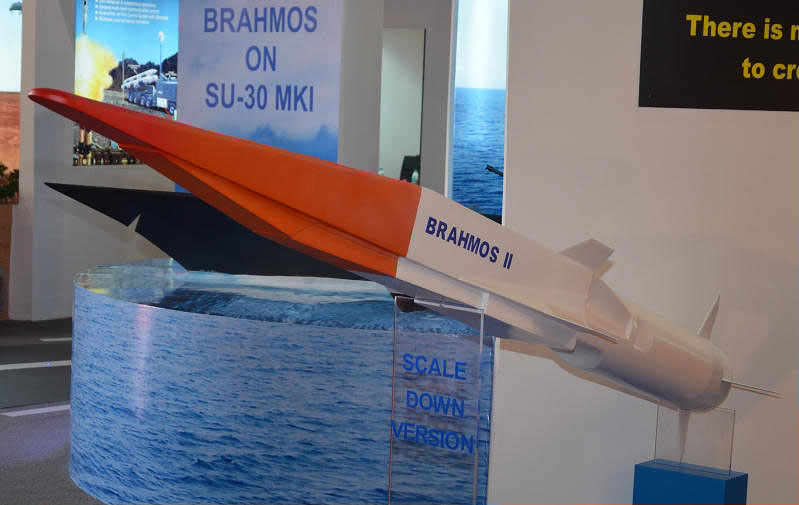
\includegraphics[width=0.44\textwidth]{figures/ch1/brahmos-II}
		\caption[Missile hypersonique BrahMos-II]{Maquette du missile de croisière hypersonique russo-indien BrahMos-II, en cours de développement : ce missile devrait atteindre une vitesse de croisière de Mach~7\footnotemark{}. Crédit : Pakistan Defence.}
		\label{fig:brahmos}
	\end{SCfigure}
	
	\footnotetext{\url{http://economictimes.indiatimes.com/news/politics-and-nation/hypersonic-version-of-brahmos-missile-on-the-way/articleshow/10286984.cms}}
	
	\subsubsection{Hétérogénéité des cibles}
	En situation réelle, un espace aérien pourrait tout à fait contenir des véhicules et autres engins volants de tous les types sus-cités, des essaims de drones très manœvrables jusqu'aux missiles balistiques les plus rapides. Un système de contrôle interactif devrait donc être assez souple pour permettre la sélection de cibles de natures très différentes.
	On peut noter que les engins volants militaires ont vocation à chercher à éviter d'être détectés, soit en étant naturellement furtifs, soit en volant à très basse altitude et en tirant parti du relief naturel. Il en résulte qu'ils peuvent n'apparaître sur les écrans de contrôle que lorsqu'ils sont déjà très proches de lieux à protéger, et peuvent éventuellement disparaître de ces écrans, offrant une fenêtre temporelle restreinte pour l'interaction.
	
	De plus, le commandant du \emph{Chevalier Paul}\footnotemark{} précise qu'outre la détection d'un aéronef, son identification est souvent très difficile, ce qui peut expliquer des accidents tels que la destruction du vol MH17\footnotemark{}. En pratique, l'équipage du \emph{Chevalier Paul} s'entraîne avec une quarantaine de cibles potentielles, mais attendu que le navire est capable de surveiller un espace aérien de plus de 500~000~km², l'on imagine aisément qu'en situation réelle, ce nombre pourrait être plus élevé, \emph{a fortiori} avec des drones en essaims.
	
	\addtocounter{footnote}{-1}
	\footnotetext{Frégate de défense aérienne (FDA) française de classe \emph{Horizon}, d'un déplacement d'environ 7000 tonnes, ayant pour mission principale de participer à la défense antiaérienne d'un groupe aéronaval, ou d'assurer la protection d'une zone ou d'un convoi contre des attaques aériennes ou de missiles.}
	\addtocounter{footnote}{1}
	\footnotetext{Abattu en Ukraine le 17 juillet 2014.}
	
	\FloatBarrier \subsection{Observations}
	Qu'il s'agisse d'applications civiles ou militaires, cette tâche est critique, puisque de nombreuses vies sont en jeu. Selon l'application, il peut donc y avoir des contraintes fermes et spécifiques, soit sur le temps de sélection maximal acceptable (contrainte de temps-réel) soit sur le taux d'erreur, ou encore sur les niveaux de zoom, etc.

	Les systèmes de contrôle aérien dont nous avons connaissance sont tous en deux dimensions, et augmentés d'informations altimétriques pour chaque engin volant. Si les contrôleurs aériens se satisfont d'un tel support, cela n'est pas sans augmenter la charge cognitive de leur tâche. S'il n'y a pas en soi de perte d'information, celle-ci est d'un accès moins immédiat. Une technique de sélection suffisamment performante pourrait rendre envisageable l'utilisation d'un système en 3D. Cela permettrait par exemple de mieux déterminer si deux avions qui paraissent dangereusement proches dans le plan le sont réellement dans l'espace, ou de pouvoir choisir un objet parmi plusieurs évoluant aux mêmes coordonnées 2D, mais à des altitudes différentes, ou tout simplement d'avoir une meilleure représentation et perception générales de la situation.
	
	Sur la base d'un système 3D, un dispositif immersif apporte \emph{a priori} des avantages supplémentaires, tant pour la perception que pour l'interaction, voire pour la représentation de l'environnement, et l'affichage de données contextuelles plus détaillées que ce qu'un dispositif de rendu 2D traditionnel permet (sans mener à un niveau d'occultation intolérable). Dans un contexte militaire, on peut également imaginer permettre à l'utilisateur, via ses interactions avec l'environnement virtuel, de fournir des informations tactiques aux forces déployées sur terre, en mer ou dans les airs.

	\begin{figure}[!htbp]
		\centering
		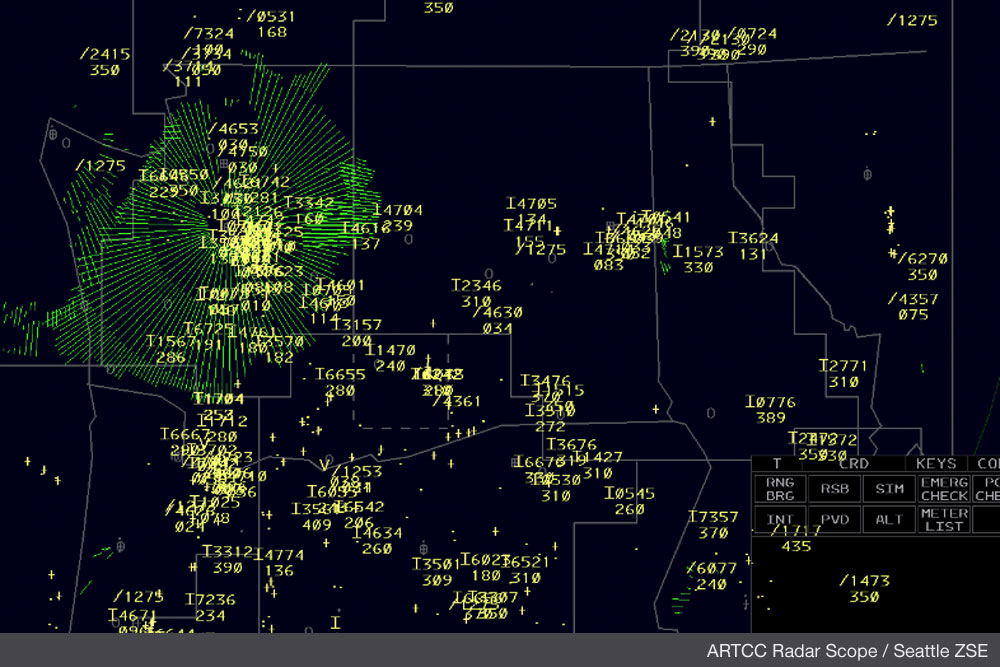
\includegraphics[width=\textwidth]{figures/ch1/Radar-Scope-ZSE}
		\caption[Écran de contrôle du trafic aérien, en 2D]{Écran de contrôle du trafic aérien. Toutes les informations, qui portent pourtant sur un espace tridimentionnel, sont représentées sur le même plan, avec une densité telle que certaines indications écrites sont illisibles. Crédit : \emph{Bold Method}.}
		\label{fig:airtraffic}
	\end{figure}
	
\section{Contrôle de l'espace maritime}
	La figure~\ref{fig:channel} représente un écran de contrôle du trafic maritime en Manche. Fondamentalement, c'est un problème très similaire à celui du contrôle du trafic aérien, car il s'agit dans les deux cas de surveiller et d'organiser un espace fluide~\cite{henninger2012avant}. Comme dans les airs, les enjeux sont à la fois militaires et civils.
	
	Les bâtiments militaires (\emph{a fortiori} s'ils sont potentiellement hostiles) doivent en effet être détectés le plus tôt possible et suivis tant qu'ils sont dans un espace d'intérêt défini, mais il faut également surveiller les bâtiments civils.
	
	Les activités commerciales normales qui font l'objet de contrôles douaniers.
	
	Cependant, la mer abrite des activités illégales diverses, incluant tous types de trafics (contrebande, œuvres d'art, drogues, armes, êtres humains) ainsi que de la piraterie ou des activités liées au terrorisme. Le fret maritime mondial représentant près de 10 milliards de tonnes, on mesure l'ampleur et l'importance du défi à l'échelle planétaire~\cite{unctad}.
	
	La piraterie, en particulier, représente un tel danger que l'Union européenne a dû mettre en place une force navale, \emph{Atalanta}\footnotemark, spécialement dédiée à la lutte contre la piraterie au large de la Somalie. Celle-ci atteint depuis quelques années un tel degré de sophistication que les pirates utilisent de grands bâtiments (cargos, chalutiers, pétroliers\ldots{}) détournés comme bateaux-mères, à partir desquels ils lancent de plus petites embarcations pour intercepter leurs cibles~\cite{audebaud2010lutte, guisnel2012pirates, dumas2015}. La Somalie n'est cependant pas le seul lieu où la piraterie sévit, puisqu'on la retrouve notamment dans le Golfe de Guinée~\cite{onuoha2012piracy}, aux abords du détroit de Malacca~\cite{raymond2009piracy} ou encore au large du Bangladesh~\cite{liss2011oceans}.
	
	\footnotetext{\url{http://eunavfor.eu/}}
	
	\begin{figure}[!htbp]
		%\centering
		\begin{subfigure}[t]{0.40\textwidth}
			\centering
			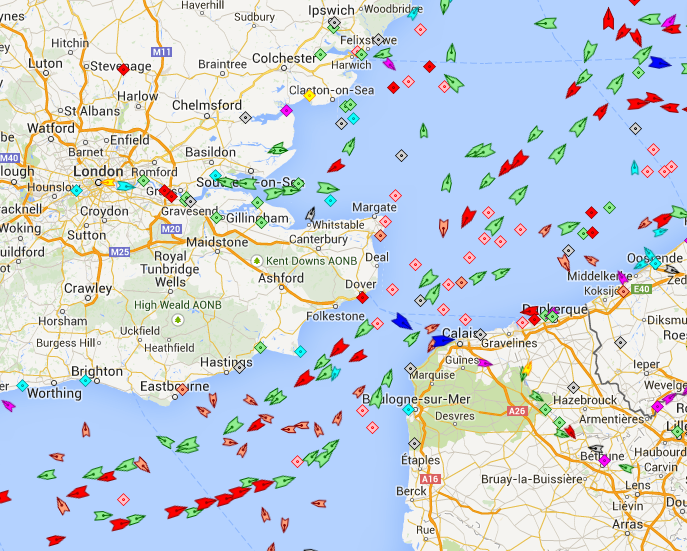
\includegraphics[width=\textwidth]{figures/ch1/channel}
			\caption[Écran de contrôle maritime en Manche (SIA)]{Écran de contrôle représentant les navires utilisant le Système d'identification automatique (SIA) en Manche. Ce système n'étant obligatoire que sur les navires de jauge brute supérieure à 300 UMS effectuant des voyages internationaux, ce n'est qu'une représentation partielle du trafic à cet instant. Crédit : \emph{Arlo Maritime}\footnotemark.}
			\label{fig:channel}
		\end{subfigure}
		~
		\begin{subfigure}[t]{0.58\textwidth}
			\centering
			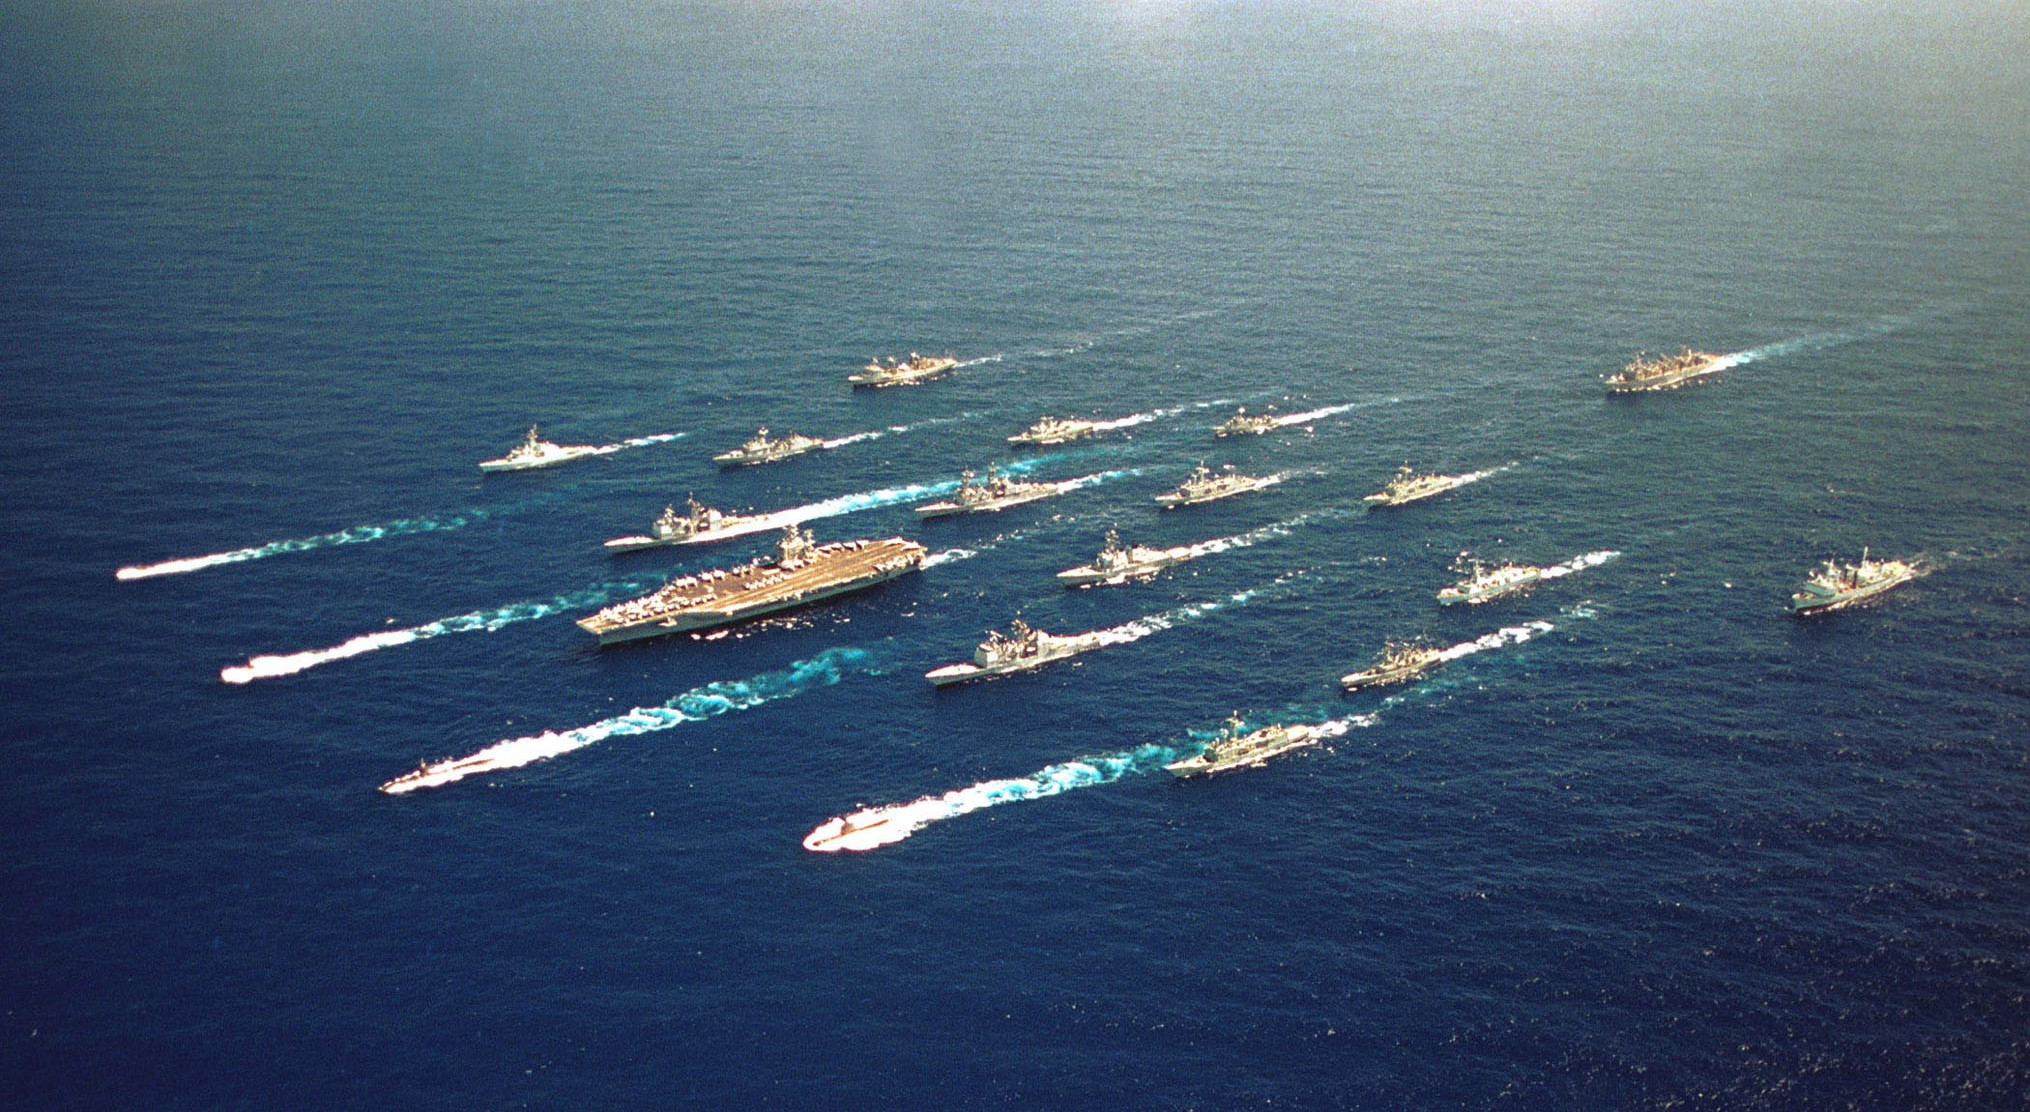
\includegraphics[width=\textwidth]{figures/ch1/lincoln}
			\caption[Le groupe aéronaval de l'USS \emph{Abraham Lincoln}]{Même dans des eaux relativement vides, la densité de navires peut être élevée localement. C'est potentiellement le cas quand un groupe aéronaval est présent, comme ici, avec le groupe aéronaval de l'USS \emph{Abraham Lincoln}, photographié en 2000. Il est de plus capital dans ce cas d'identifier clairement tous les navires présents, compte tenu de leur importance militaire, sous-marins compris. On précisera toutefois qu'en situation réelle, les navires sont généralement plus espacés que cela. Crédit : Gabriel Wilson, via \emph{Wikimedia}.}
			\label{fig:lincoln}
		\end{subfigure}
		\label{fig:muddyWaters}
		\caption{Densité de cibles dans les espaces maritimes.}
	\end{figure}
	
	\footnotetext{\url{http://www.arlomaritime.com}}
	
	La protection environnementale nécessite également un contrôle strict de l'espace maritime, notamment pour éviter le deversement de polluants en mer, particulièrement d'hydrocarbures.
	
	\FloatBarrier \subsection{Difficultés}
	La plupart des navires se déplacent à la surface de l'eau. Par conséquent, leur représentation dans le plan sur un écran de contrôle n'implique généralement pas de perte d'information significative, contrairement au cas aérien. Les sous-marins constituent toutefois une exception à cette règle, et peuvent plonger à plusieurs centaines de mètres. S'ils représentent une très petite minorité des navires en circulation, leur détection revêt une importance militaire critique.
	
	\subsubsection{Données 3D affichées en 2D}
	De fait, le problème de l'affichage planaire d'informations tridimensionnelles demeure, même s'il est moins prégnant. Les navires sont en moyenne bien plus lents que les aéronefs, mais certains bateaux de type \emph{go-fast} peuvent dépasser les 150~km/h. Ces navires étant fréquemment utilisés par les trafiquants de drogues pour échapper aux garde-côtes, il est particulièrement important de pouvoir les détecter et les contrôler.
	
	\subsubsection{Densité d'informations}
	Comme souvent pour les tâches de ce type, la densité de cibles dépend du niveau de zoom, qui peut résulter d'un choix de l'utilisateur, ou d'une contrainte (l'obligation d'avoir en permanence une zone donnée affichée, par exemple). La densité peut donc varier et, potentiellement, être très élevée. Elle devient particulièrement problématique lorsque l'on souhaite afficher des informations contextuelles à propos des navires, ou d'un sous-ensemble de ceux-ci. Ces informations peuvent concerner le type du navire, son pavillon, son propriétaire, son équipage, son origine, sa destination (connue ou présumée) ses escales, sa cargaison, etc., ainsi que les éventuelles précédentes valeurs de toutes ces données.
	
	\subsubsection{Vitesse et contraintes de temps}
	Ces informations revêtent une importance particulière lorsqu'il est nécessaire aux autorités de faire la différence entre un bateau effectuant un simple voyage de plaisance et une embarcation susceptible d'être engagée dans une activité criminelle. Un groupe de \emph{speedboats} filant à vive allure vers une destination donnée peut tout aussi bien être un groupe d'amis en promenade qu'une bande de trafiquants de drogues. Il est donc nécessaire aux agents de contrôle de l'espace maritime de disposer d'un maximum d'informations le plus vite possible pour déterminer s'il faut ordonner l'interception de ces bateaux.
	
	La figure~\ref{fig:lincoln} illustre un cas de forte densité locale de navires, avec des cibles de haute importance stratégique de surcroît. Près des ports, la densité peut être plus élevée encore, même si les navires concernés sont moins préoccupants pour les autorités. Il leur est toutefois nécessaire de garantir la circulation fluide et sûre de ces navires, et de veiller à ce que personne ne tire parti de cette forte densité à des fins illicites ou criminelles.
	
	\section{Contrôle de l'espace extra-atmosphérique}
	Le problème de la surveillance de l'espace extra-atmosphérique se pose de façon assez analogue à celui des espaces aérien et maritime. Là encore il s'agit d'une part de vérifier que les objets qui s'y meuvent le font de façon sûre, et d'identifier ce qui peut potentiellement représenter une menace (essentiellement militaire, car à ce jour aucune organisation criminelle connue n'a pu mettre un objet en orbite).
	
	Même si d'importantes restrictions sont en place sur l'utilisation de l'espace extra-atmosphérique à des fins militaires\footnotemark, les missiles balistiques, en particulier intercontinentaux, passent par ce milieu. Il est donc nécessaire aux systèmes de détection et de défense de pouvoir les distinguer rapidement des satellites. Compte tenu de l'extrême dangerosité de ces armes, et de leur vitesse foudroyante, tout système interactif permettant à un être humain d'examiner la situation afin de prendre une décision se doit d'être extrêmement performant, c'est-à-dire de permettre un examen approfondi de la cible visée par l'utilisateur aussi rapidement que possible, et en minimisant les erreurs de sélection. Un tel missile est représenté sur la figure~\ref{fig:m51}.
	
	Par ailleurs, une pratique consistant à utiliser un satellite pour se rapprocher au plus près d'un autre afin de l'observer et d'espionner ses activités se développe de plus en plus. Nous sommes donc ici dans un cas où, sur un écran de surveillance --- à supposer que l'on puisse détecter cela --- les deux cibles (le satellite espion et le satellite espionné) apparaîtraient avec des trajectoires quasi identiques, et très, très proches l'une de l'autre, voire superposées, si un satellite est juste au-dessus de l'autre, par exemple.
	
	\footnotetext{\emph{Treaty on Principles Governing the Activities of States in the Exploration and Use of Outer Space, including the Moon and Other Celestial Bodies} -- \url{http://disarmament.un.org/treaties/t/outer_space}}
	
	\FloatBarrier \subsection{Débris}
	D'après l'Agence spatiale européenne (ESA, d'après son sigle anglophone), l'orbite terrestre compterait environ 29~000 objets de plus de 10~cm, 670~000 objets de plus de 1~cm, et pas moins de 170 millions d'objets de plus de 1~mm\ldots{} La collision d'un satellite artificiel avec un objet de seulement un millimètre pourrait détruire un sous-système, tandis qu'un objet d'un centimètre détruirait généralement le satellite\footnotemark.
	\footnotetext{\url{http://www.esa.int/Our_Activities/Space_Engineering_Technology/Clean_Space/How_many_space_debris_objects_are_currently_in_orbit}}
	
	Les débris spatiaux proviennent de sources aussi diverses que des véhicules spatiaux hors service, de l'équipement perdu (voir figure~\ref{fig:spaceDeb}), des propulseurs de véhicules\ldots{} ou des armes\footnotemark~\cite{chun1999shooting}.
	
	\footnotetext{\emph{Space Debris from Anti-Satellite Weapons} -- \url{http://www.ucsusa.org/sites/default/files/legacy/assets/documents/nwgs/debris-in-brief-factsheet.pdf}}
	
	Si le sujet est préoccupant pour les satellites et autres vols non habités, il est beaucoup plus inquiétant pour les vols habités. La question est d'autant plus importante que les vols habités pourraient devenir bien plus courants à moyen terme\footnotemark.
	
	\footnotetext{\emph{SpaceX's Elon Musk Unveils Interplanetary Spaceship to Colonize Mars} -- \url{http://www.space.com/34210-elon-musk-unveils-spacex-mars-colony-ship.html}}
	
	La question des débris, et plus généralement des collisions et de la circulation dans l'espace extra-atmosphérique est suffisamment sérieuse pour que la \emph{Federal Aviation Administration} (FAA) des États-Unis travaille sur un système civil de gestion du trafic spatial\footnotemark.
	
	\footnotetext{\emph{Towards a Civil Space Traffic Management System} -- \url{https://www.faa.gov/about/office_org/headquarters_offices/ast/media/6_space_traffic_management_plans.pdf} ;
	
	\emph{Congress gets report on giving FAA space traffic role} -- \url{http://spacenews.com/congress-gets-report-on-giving-faa-space-traffic-role}}
	
	\begin{figure}[!htbp]
		%\centering
        \begin{subfigure}[t]{0.41\textwidth}
            \centering
            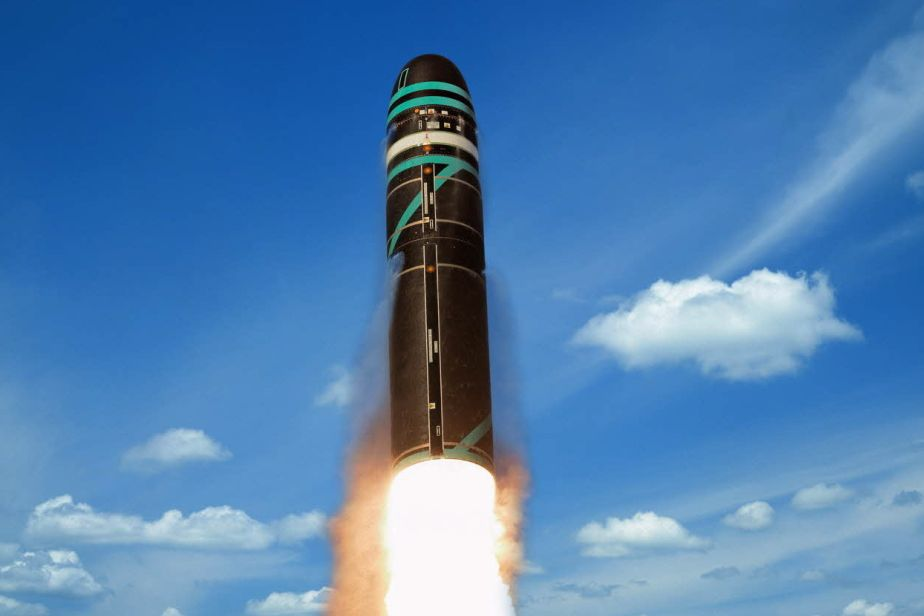
\includegraphics[width=\textwidth]{figures/ch1/m51}
        	\caption[Missile français M51]{Tir du missile balistique français M51, depuis un sous-marin. Son altitude de croisière est d'environ 1000~km et sa vitesse maximale serait de Mach~25\footnotemark. Crédit : \emph{Defence Talk}\footnotemark.}
            \label{fig:m51}
        \end{subfigure}
        ~
        \begin{subfigure}[t]{0.57\textwidth}
            \centering
            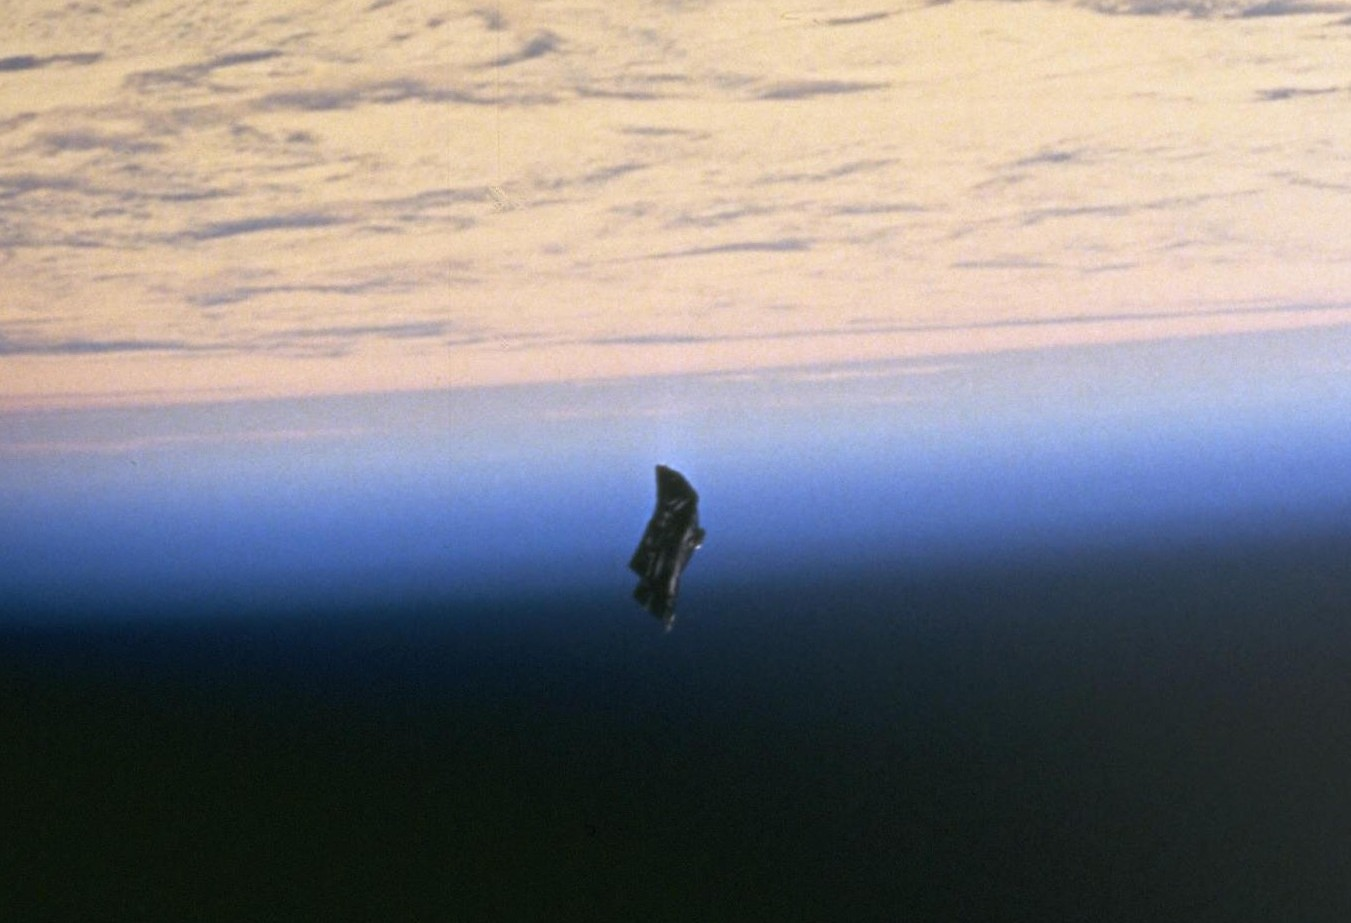
\includegraphics[width=\textwidth]{figures/ch1/space_debris_zoom}
            \caption[Débris spatial]{Débris spatial : une couverture thermique à la dérive en orbite terrestre. Crédit : NASA\protect\footnotemark.}
            \label{fig:spaceDeb}
        \end{subfigure}
        \label{fig:aerospace}
        \caption{Objets aérospatiaux.}
	\end{figure}
	
	\addtocounter{footnote}{-2}
	\footnotetext{\url{http://www.techno-science.net/?onglet=glossaire&definition=12366}}
	\addtocounter{footnote}{1}
	\footnotetext{\url{http://www.defencetalk.com/french-m51-ballistic-missile-self-destructs-in-failed-test-47689}}
	\addtocounter{footnote}{1}
	\footnotetext{\url{https://eol.jsc.nasa.gov/SearchPhotos/photo.pl?mission=STS088&roll=724&frame=66}}
	
	\subsection{Observations}
	L'espace extra-atmosphérique présente de très nombreux objets d'intérêt, ayant des caractéristiques variées, et dont la détection peut être critique. Un système de sélection adapté devrait donc pouvoir gérer l'hétérogénéité des cibles potentielles et garantir des performances minimales pour les cas les plus importants.	
	
	\section{Vidéo-surveillance}
	La vidéo-surveillance s'applique aussi bien aux foules dans les lieux publics ou sensibles qu'à la voirie, où peuvent circuler des véhicules de types divers. Un agent de sécurité en charge de visionner un flux de vidéo-surveillance pourrait avoir à sélectionner une personne, par exemple pour obtenir des informations sur celle-ci grâce à la reconnaissance faciale, ou un véhicule, pour les mêmes raisons, par exemple grâce à sa plaque d'immatriculation.
	
	Quelle que soit la nature de la cible, sa sélection pourrait avoir pour but de zoomer dessus, de verrouiller une caméra robotisée afin qu'elle la suive, ou de la désigner à des forces de sécurité sur le terrain pour qu'elles interviennent physiquement. Le suivi de cibles filmées par des caméras de vidéo-surveillance a déjà fait l'objet de travaux de recherche~\cite{lipton1998moving, nishimura1997video, benfold2011stable}, mais plus rarement avec composante interactive qui nous intéresse ici.
	
	Une des difficultés de cette application est le fait qu'une cible peut bouger non seulement de façon imprévisible, mais également de façon totalement indépendante des actions de l'utilisateur~\cite{ilich2010moving, silva2012real}.	
	
	\FloatBarrier \subsection{Piétons et foules}
	La vitesse d'un être humain à pied est (généralement très) inférieure à 45~km/h. Les changements de direction peuvent aller jusqu'au demi-tour, et leur fréquence est très variable selon la tâche accomplie. On peut supposer que cette fréquence est au plus de l'ordre de quelques Hz, en pratique souvent bien moins.
	
	Dans certains cas, par exemple au cours de manifestations publiques ou de concerts, les individus filmés peuvent devenir quasi statiques, mais très nombreux et confinés dans un espace réduit. Il en résulte une densité de cibles potentielles et un niveau d'occultation très élevés. Dans ces circonstances, la vidéo-surveillance devient difficile.

	\FloatBarrier \subsection{Véhicules motorisés}
	Sur la voie publique, un véhicule motorisé n'est pas censé dépasser 130~km/h, exception faite de ceux qui enfreignent le code de la route. Mais, soit à cause de l'infraction en question, soit parce qu'ils l'enfreignent pour fuir après des délits ou crimes plus graves, ces véhicules-là peuvent justement faire l'objet d'une attention particulière de la part des forces de l'ordre. Dans ces cas-là, la vitesse d'un véhicule peut dépasser les 300~km/h\footnotemark.
	
	\footnotetext{\emph{Un chauffard roule à plus de 320~km/h sur l'A1} -- \url{http://www.rts.ch/info/suisse/3483170-un-chauffard-roule-a-plus-de-320-km-h-sur-l-a1.html}}
	
	Les changements de direction dépendent évidemment de la vitesse. En ville, à moins de 50~km/h, une automobile peut effectuer un virage à 90 degrés dans un laps de temps de l'ordre de la seconde si sa vitesse est réduite, mais elle est contrainte à des courbes beaucoup plus douces lorsqu'elle se déplace rapidement, par exemple sur une autoroute.
	
	La fréquence des changements de direction dépend également de la vitesse, tant pour des raisons physiques que du fait du tracé des trajets communément effectués. En milieu urbain dense, on peut considérer qu'un véhicule va changer de direction, de façon plus ou moins prononcée, à une fréquence de l'ordre de 0,1~Hz, sachant qu'en cas de nécessité, cette fréquence peut être nettement plus élevée.
	
	\FloatBarrier \subsection{Véhicules divers}
	En plus des piétons et des automobiles, la vidéo-surveillance s'applique à tous les véhicules et moyens de déplacement susceptibles d'être utilisés dans l'espace public : patins à roulettes, skateboards de tous types, bicyclettes, motocyclettes, etc. Les caractéristiques du mouvement de ces moyens de transport sont diverses, mais généralement comprises dans les intervalles formés par les piétons et les automobiles. Il est donc important qu'une technique de sélection puisse non seulement gérer les valeurs extrêmes de vitesse, d'angle et de fréquence de changements de direction, mais également les diverses combinaisons de ces valeurs qui peuvent se présenter simultanément.
		
	\begin{figure}[!htbp]
		%\centering
		\begin{subfigure}[t]{0.49\textwidth}
			\centering
			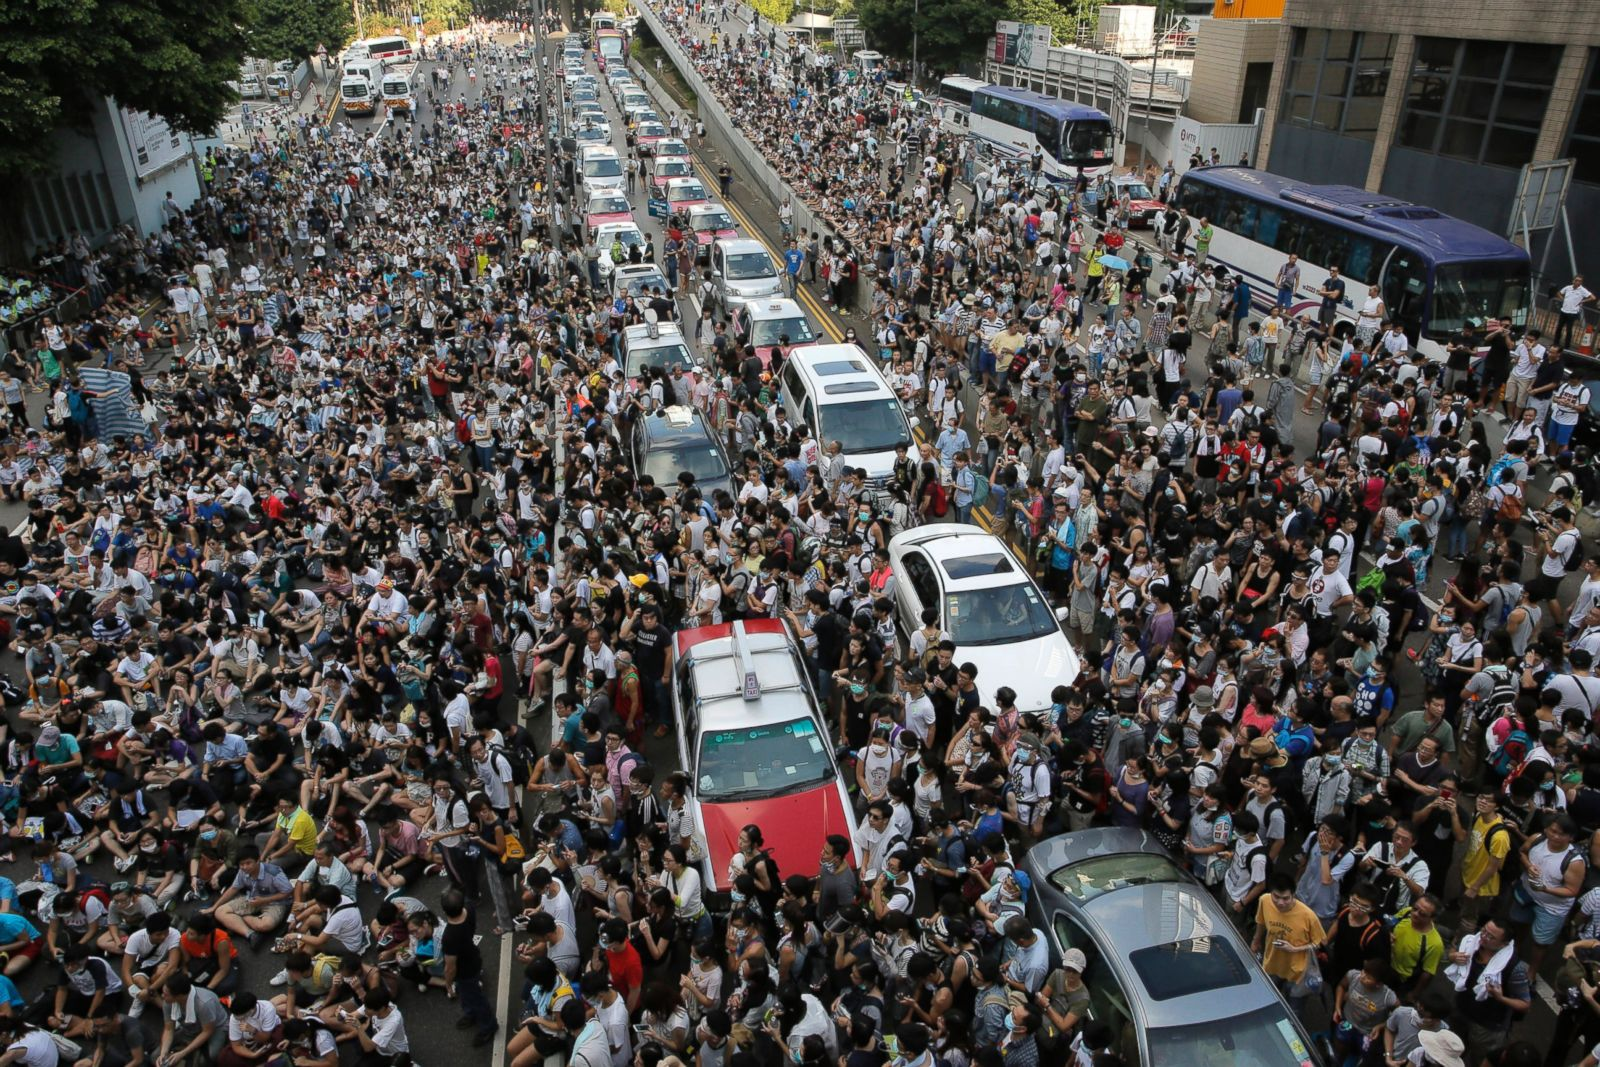
\includegraphics[width=\textwidth]{figures/ch1/crowdhk}
			\caption[Foule de manifestants à Hong-Kong]{Foule de manifestants à Hong-Kong. Le mouvement des individus est en moyenne très faible, mais leur densité est très élevée. Crédit : \emph{ABC News}.}
			\label{fig:crowdhk}
		\end{subfigure}
		~
		\begin{subfigure}[t]{0.49\textwidth}
			\centering
			\includegraphics[width=\textwidth]{figures/ch1/crowdacdc}
			\caption[Foule à un concert]{Foule à un concert du groupe AC/DC. Le mouvement presque nul, mais la densité de cibles est extrêmement élevée. Crédit : \emph{SHP Online}\footnotemark.}
			\label{fig:crowdacdc}
		\end{subfigure}
		\label{fig:crowds}
		\caption{Foules.}
	\end{figure}
	

	\footnotetext{\url{http://www.shponline.co.uk/understanding-crowds-and-crowded-space-issues}}
	
	\section{Surveillance électromagnétique}
	La surveillance s'applique également à la partie invisible du spectre électromagnétique, et notamment aux signaux émis par les téléphones portables. Les objectifs de cette surveillance sont multiples mais peuvent inclure la lutte contre la criminalité, le terrorisme, ou un adversaire militaire, mais aussi l'étude des usages afin d'adapter les réseaux de communication, de transport, etc.	
	
	\FloatBarrier \subsection{Moyens et méthodes}
	La figure~\ref{fig:cellphones} fournit une illustration (tirée d'une œuvre de fiction) d'un tel système. S'il est présenté dans l'œuvre en question comme fondé sur des détections par satellite, en pratique les systèmes réels se fondent plutôt sur des capteurs aériens ou, plus simplement, sur les données fournies directement par les opérateurs téléphoniques, comme le permet par exemple l'article 20 de la loi de programmation militaire de décembre 2013, en France\footnotemark.
	
	\footnotetext{\url{https://www.legifrance.gouv.fr/affichTexte.do?cidTexte=JORFTEXT000028338825}}
	
	L'État français s'appuie notamment sur les services d'entreprises telles que Deveryware :
	
	\begin{displayquote}
		[Celle-ci] est depuis 2003 la spécialiste de référence pour le développement et le déploiement de solutions mettant en œuvre la géolocalisation en temps réel des personnes et des biens.

		Elle est un partenaire important de l'État français pour des applications régaliennes utilisant ces techniques, qu'il s'agisse de sécurité publique ou de sécurité civile pour contribuer à la mise en sécurité des citoyens.\footnotemark
	\end{displayquote}
	
	\footnotetext{\url{http://www.deveryware.com/savoir-faire/notre-expertise}}
	
	\begin{figure}[!htbp]
		\centering
		\includegraphics[width=\textwidth]{figures/ch1/cellphones}
		\caption[Surveillance des signaux de téléphones portables]{Illustration d'un système de surveillance en temps réel des signaux émis par les téléphones portables, tiré de la série télévisée \emph{Le Bureau des légendes}, et inspiré de systèmes réels (dont les images ne sont pas publiques). Sur cette image représentant une vue de la ville d'Alger, chaque point coloré représente la position d'un téléphone portable dont le signal est capté et localisé. Le nombre de cibles potentielles est très élevé, et la densité peut être extrême par endroits. \OE{}uvre réalisée par Éric Rochant et produite par Canal+.}
		\label{fig:cellphones}
	\end{figure}
	
	\FloatBarrier \subsection{Hétérogénéité}
	L'on comprend aisément que la surveillance des signaux téléphoniques porte sur des cibles à peu près identiques à celles de la vidéo-surveillance. En effet, les téléphones sont généralement transportés par des gens à pied, en voiture, à vélo, dans les transports en commun, etc. Cependant, une difficulté s'ajoute puisque l'on surveille ici des espaces beaucoup plus grands, et donc plus hétérogènes.
	
	En sus de la quantité de cibles, il faut donc pouvoir gérer leur très forte densité, et l'hétérogénéité de leurs mouvements : un groupe de piétons peut potentiellement être à seulement quelques mètres d'un groupe de voyageurs dans un train à grande vitesse, d'automobilistes sur une autoroute, etc.
	
	\FloatBarrier \subsection{Informations complémentaires}
	Par ailleurs, il peut être souhaitable ou nécessaire d'afficher des informations complémentaires pour chaque signal localisé. L'identité ou la localisation de l'interlocuteur si un appel est en cours, la durée de l'appel, la fréquence à laquelle l'interlocuteur courant est appelé, la liste des interlocuteurs fréquents de la personne concernée, les localisations de ces interlocuteurs fréquents, leurs interlocuteurs à eux — en somme, le réseau social de la personne observée — ne sont que des exemples parmi d'autres.
	
	Ces informations pourraient être affichées sous forme de texte associé à un point, ou représentées par d'autres moyens graphiques : traits entre les signaux, clignotements, textures, etc. Dans tous les cas, la complexité visuelle et la densité de la vue présentée à l'utilisateur n'en seraient qu'accrues ; de fait, la difficulté de la tâche de sélection le serait aussi. Nous sommes donc face à une tâche de sélection de cibles mobiles très nombreuses, denses, hétérogènes dans un environnement visuel pouvant contenir de nombreuses informations complémentaires.
	
	\section{Interaction avec des gestes sportifs ou artistiques}	
	Les retransmissions d'événements sportifs présentent un potentiel d'interactivité intéressant, et nécessitent souvent la sélection de cibles mobiles~\cite{ilich2010moving}. Il peut être utile, par exemple, de sélectionner un joueur de football pour afficher ses statistiques. Pour les mêmes raisons, un ballon ou une balle peuvent être une cible, de même que certains éléments du terrain de jeu, qui sont physiquement fixes mais peuvent être mobiles à l'écran du fait des mouvements de caméra. La nature du mouvement de ces cibles varie nécessairement d'un sport ou d'un jeu à l'autre.
	
	\FloatBarrier \subsection{Athlètes}
	
	Certains sports d'équipe comme le football, le hockey sur glace ou le basket-ball sont caractérisés par des cibles potentielles relativement nombreuses, mobiles, et dont les mouvements ne sont pas toujours très prévisibles. Les mouvements d'humains à pied obéissent aux règles habituelles, mais dans un cadre sportif, ils peuvent être sur des patins à glace, des bicyclettes, des skis, etc. Les athlètes peuvent donc avoir des mouvements nettement plus rapides que de simples piétons, jusqu'à plus de 160~km/h pour certains skieurs\footnotemark.
	
	\footnotetext{\url{http://www.swissinfo.ch/fre/societe/ski-alpin-_une-histoire-de-famille-se-termine-au-lauberhorn/37746484}}
	
	\begin{figure}[!htbp]
		\centering
		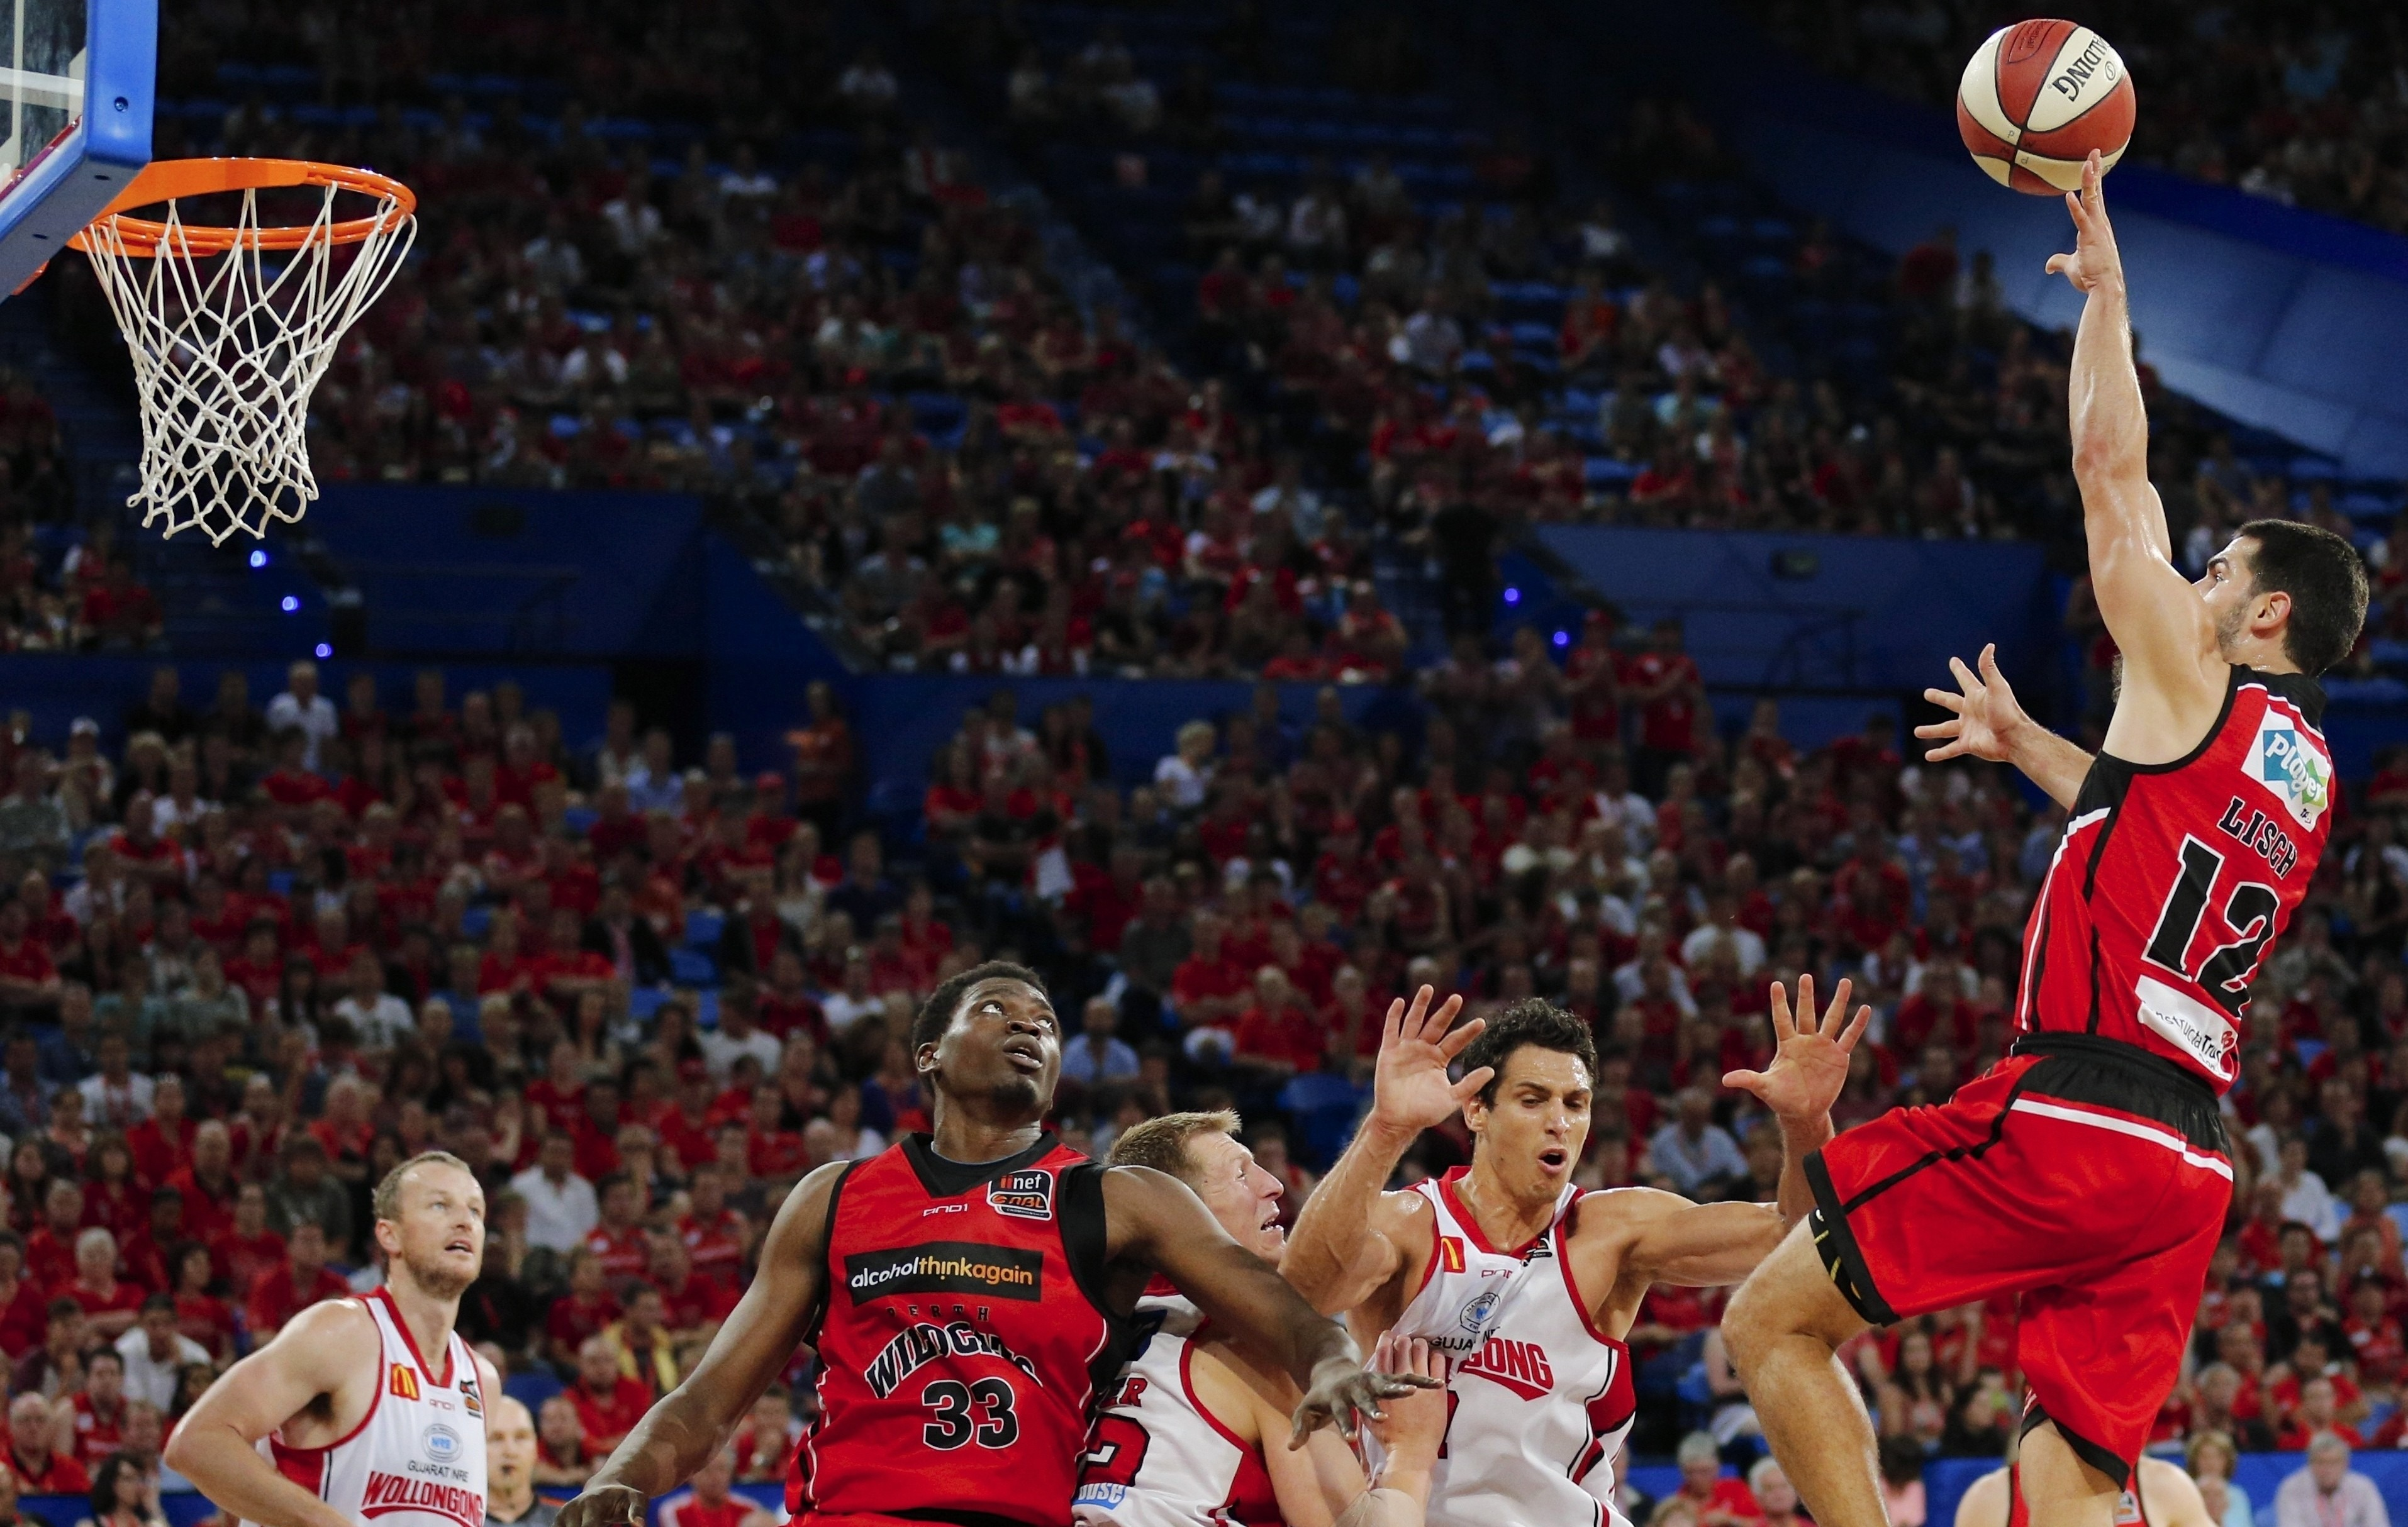
\includegraphics[width=0.60\textwidth]{figures/ch1/basket}
		\caption[Match de basket-ball]{Match de basket-ball. Les joueurs sont peu nombreux, mais vifs et imprévisibles. Ils sont très près les uns des autres et s'occultent mutuellement, surtout filmés depuis le côté. Le ballon lui-même peut être une cible, plus rapide et imprévisible encore. Crédit : \emph{Weekend Notes}\footnotemark.}
		\label{fig:basketball}
	\end{figure}
	
	\footnotetext{\url{http://www.weekendnotes.com/perth-wildcats-nbl-games}}
	
	\FloatBarrier \subsection{Véhicules}
	Les valeurs deviennent plus extrêmes encore dans les sports hippiques ou mécaniques. Dans ces derniers cas, les mouvements sont certes (souvent) plus prévisibles, mais aussi nettement plus rapides, avec en plus une certaine tendance des cibles à être très proches les unes des autres, ce qui augmente la probabilité d'erreur de sélection. Et si l'on inclut les courses de drones aériens\footnotemark{} (une discipline récente et en plein essor) dans les sports mécaniques, l'on est alors face à un cas où les objets sont à la fois très rapides et très manœuvrables, donc potentiellement imprévisibles dans leurs mouvements.
	
	\footnotetext{\url{https://thedroneracingleague.com}}
	
	\FloatBarrier \subsection{Projectiles}
	Les divers projectiles utilisés dans les sports (balles, ballons, volants, palets, etc.) sont généralement beaucoup plus petits et rapides que les joueurs, ce qui en fait des cibles très difficiles. Un palet de hockey sur glace, par exemple, peut dépasser les 180~km/h\footnotemark{}, une balle de baseball peut atteindre 199~km/h\footnotemark{}, tandis qu'une balle de tennis peut excéder 260~km/h\footnotemark{}, et une balle de golfe peut (presque) atteindre 350~km/h\footnotemark{}. Dans le cas du hockey sur glace, les rebonds potentiellement nombreux du palet peuvent rendre sa trajectoire complexe et imprévisible. Dans une moindre mesure, c'est vrai d'une balle de baseball, voire d'un ballon de football, par exemple.
	
	Cependant, il n'y a généralement qu'un seul projectile de ce type par match, donc dans la mesure du possible, un raccourci dédié (éventuellement actionné à l'aide d'un contrôle spécifique) serait probablement une option préférable à l'utilisation d'une technique de sélection \og libre \fg{}, fût-elle assistée.
	
	\addtocounter{footnote}{-3}
	\footnotetext{\url{https://sports.yahoo.com/blogs/nhl-puck-daddy/khl-alexander-ryazantsev-sets-world-record-hardest-shot-174131642.html}}
	
	\addtocounter{footnote}{1}
	\footnotetext{\url{http://m.mlb.com/cutfour/2016/06/10/183198514/giancarlo-stanton-hits-hardest-ball-recorded-by-statcast}}
	
	\addtocounter{footnote}{1}
	\footnotetext{\url{http://www.smh.com.au/sport/tennis/aussie-smashes-tennis-serve-speed-record-20120513-1ykfk.html}}
	
	\addtocounter{footnote}{1}
	\footnotetext{\url{http://www.guinnessworldrecords.com/world-records/fastest-golf-drive}}
	
	Le billard, sous ses diverses formes (\emph{pool}, \emph{snooker}, etc.) est intéressant en ce que, d'une part, les \og projectiles \fg{}, c'est-à-dire les boules, sont en relativement grand nombre, et ne peuvent donc bénéficier d'un raccourci dédié, et d'autre part, leurs mouvements sont extrêmement vifs et difficiles à prédire. En effet, le premier segment d'une trajectoire de boule peut ne durer que 0,12~seconde\footnotemark{}.
	
	\footnotetext{\emph{Faster Than a Speeding Bullet?} -- \url{http://www.sfbilliards.com/Misc/onoda_all_txt.pdf}}
	
	Citons également les courses de billes dans le sable (\emph{sand marble racing}), un jeu curieux qui consiste à laisser rouler plusieurs billes dans des sillons creusés dans le sable dont le tracé est soigneusement étudier pour créer une sensation de suspense concernant l'issue de la \og course \fg{}. Ce passe-temps plus intéressant qu'il peut en avoir l'air donne lieu à des enregistrements vidéo largement diffusés sur internet\footnotemark{}, agrémentés de statistiques, et tout à fait susceptibles d'être augmentés par des capacités d'interaction qui nécessiteraient la sélection de ces objets rapides aux mouvements vifs.
	
	\footnotetext{\emph{Sand marble races are a lot more thrilling than I thought they would be}
	
	\url{https://www.reddit.com/r/videos/comments/6linoy/sand_marble_races_are_a_lot_more_thrilling_than_i}}

	\FloatBarrier	
	\section{Jeux vidéo}
	La sélection ou le pointage de cibles mobiles est une tâche que l'on retrouve dans de très nombreux jeux vidéo, appartenant à un nombre important de catégories. On peut notamment citer les jeux de tir, les jeux de rôle d'action, les jeux de gestion, ou de stratégie et tactique militaire, les simulateurs de vol de combat, ainsi que les jeux de type arène de bataille en ligne multijoueur.
	
	D'un type de jeu à l'autre, la sélection de cibles varie à la fois du fait de la nature des cibles et parce que la tâche elle-même n'est pas vue de la même façon. Si elle est un élément essentiel des mécanismes du jeu dans certains genres, avec une valeur ludique propre, dans d'autres, elle est purement utilitaire, comme nous allons le voir dans les sous-sections suivantes.
	
	\subsection{Jeux de tir}
	Dans un jeu de tir à la première personne (\emph{First-person shooters}, ou FPS, comme \emph{Doom}, \emph{Counter-Strike}\ldots{} et \emph{Third-person shooters}, ou TPS, comme \emph{Max Payne}, \emph{Gears of War}\ldots{}) la caméra est placée \og dans la tête \fg{} du personnage, selon un mode appelé vue subjective ; dans un TPS, la caméra est placée hors du personnage, souvent derrière lui, on parle alors de objective. Un FPS et un TPS sont présentés sur la figure~\ref{fig:shooters}.
	
	\begin{figure}[!htbp]
		%\centering
		\begin{subfigure}[t]{0.49\textwidth}
			\centering
			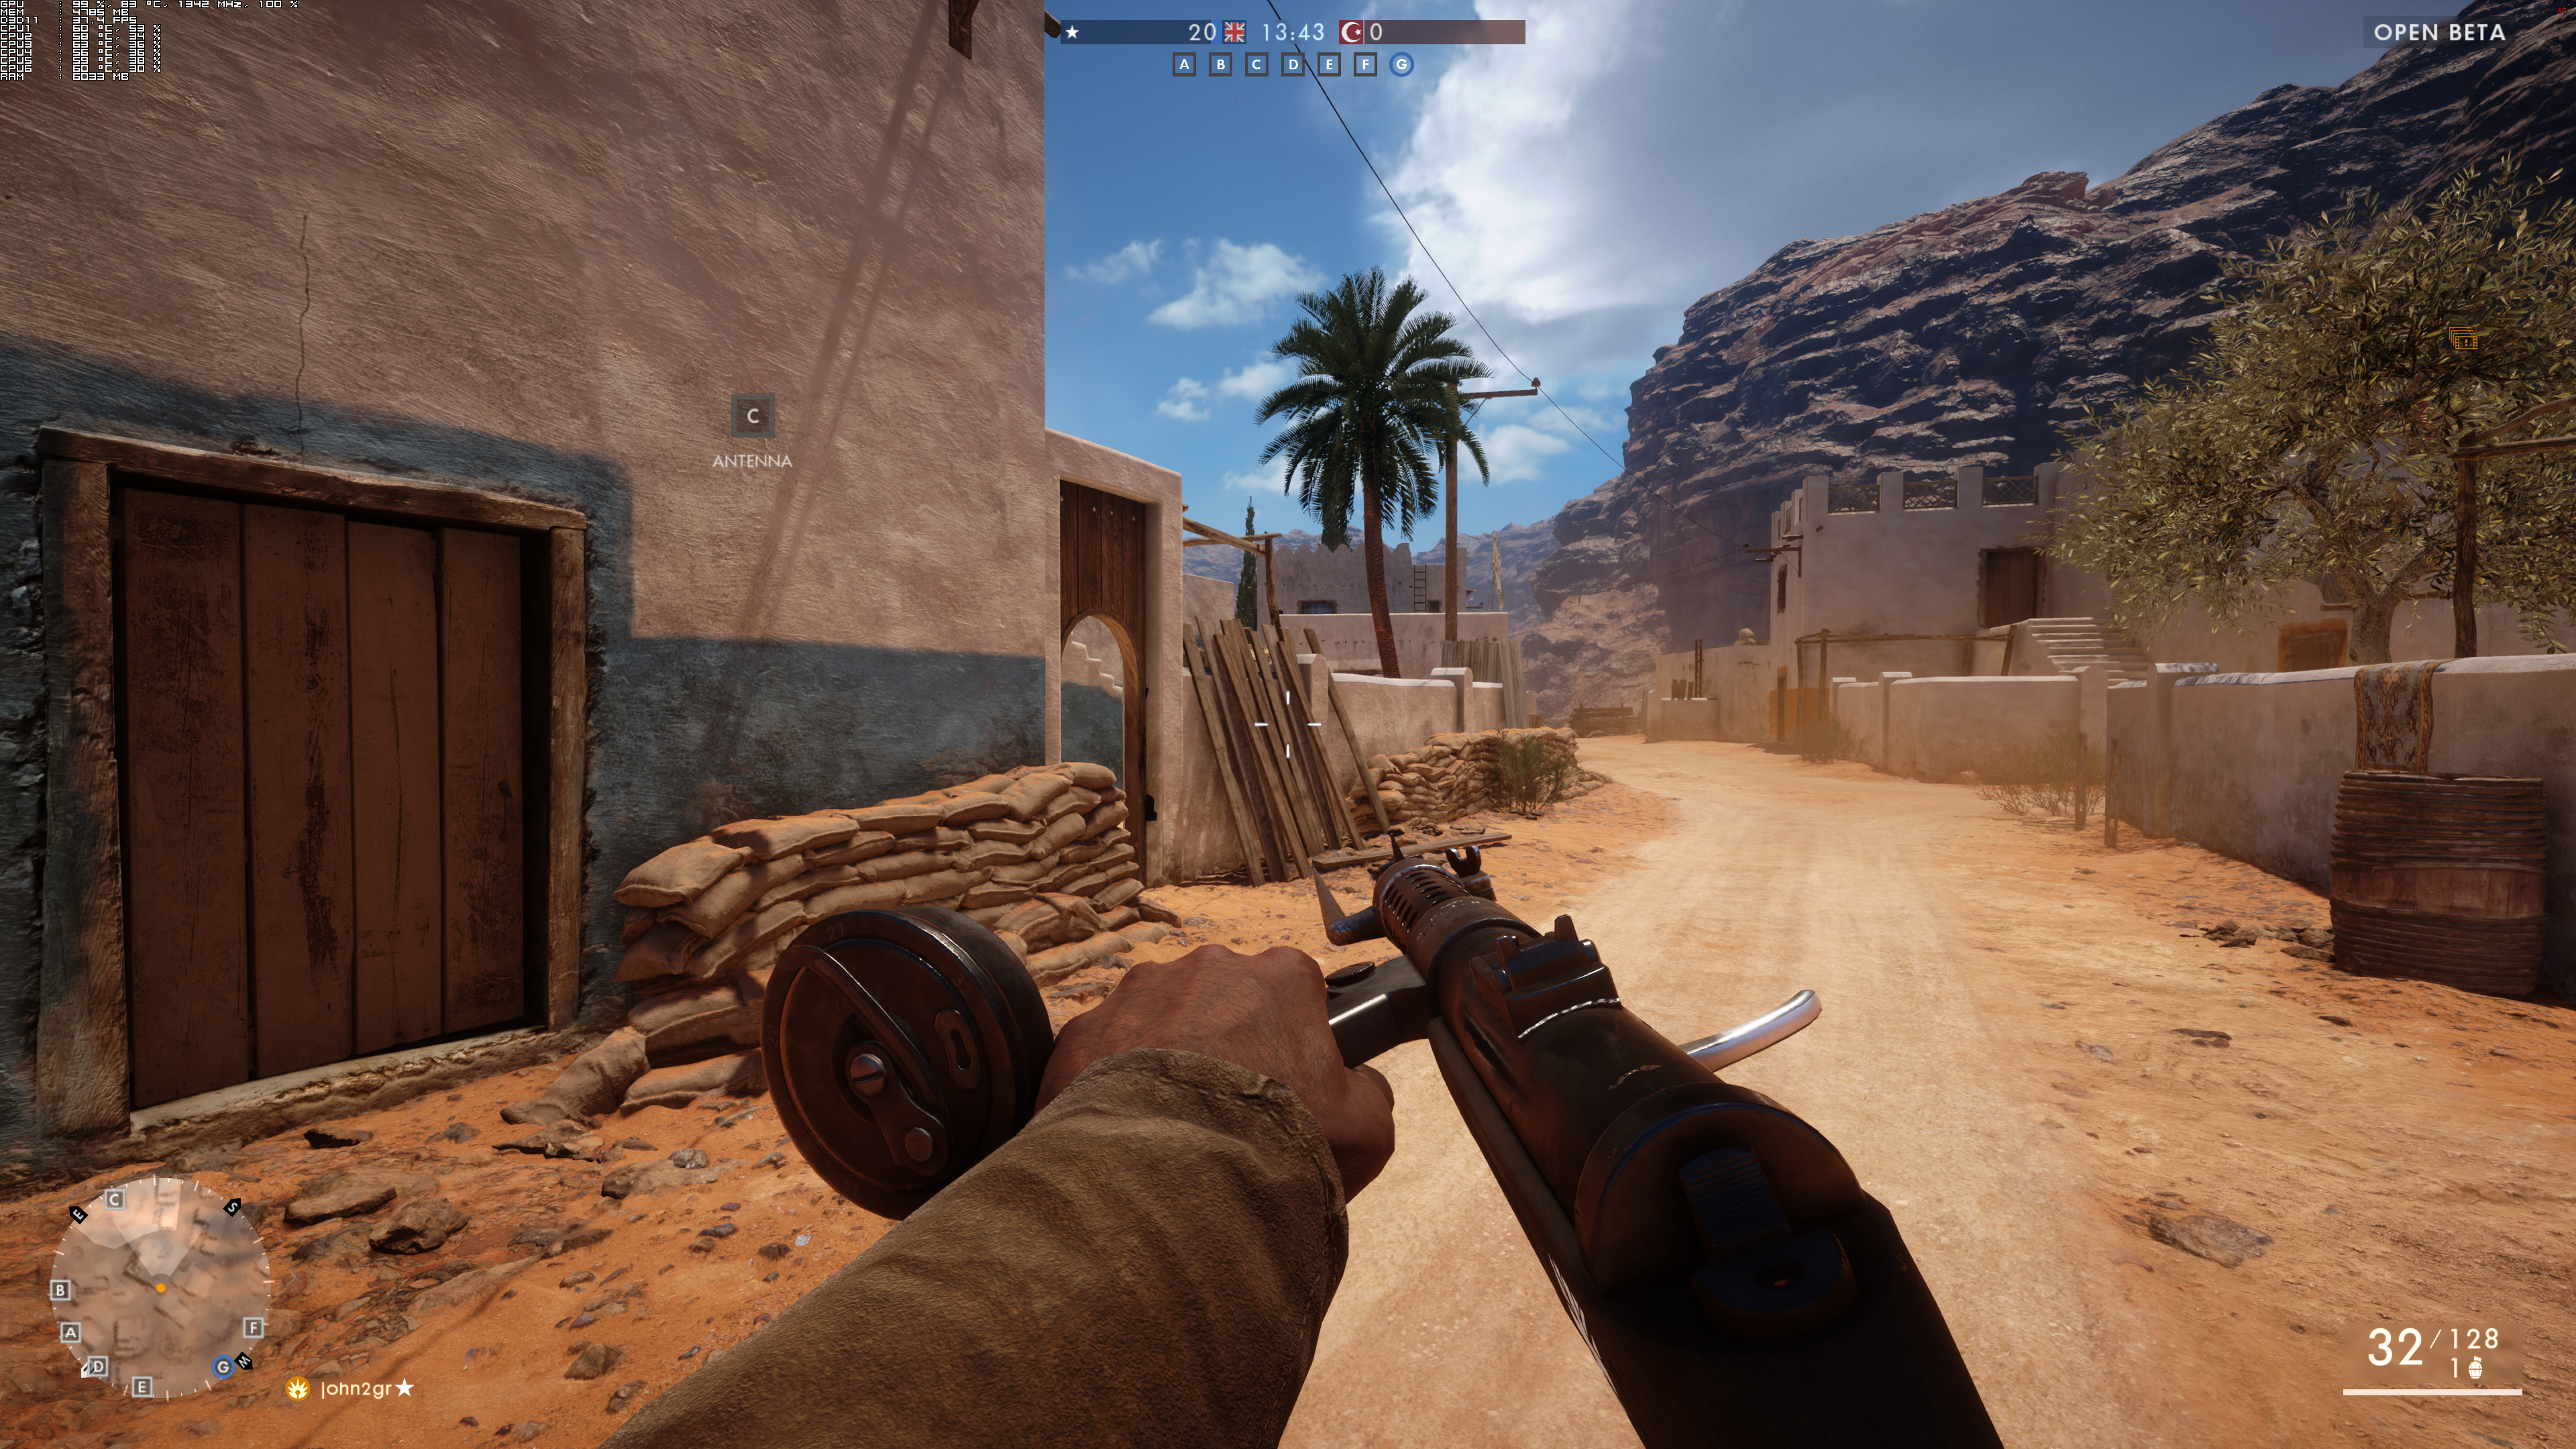
\includegraphics[width=\textwidth]{figures/ch1/bf1}
			\caption[Le FPS \emph{Battlefield 1}]{Le FPS \emph{Battlefield 1}. Des ennemis peuvent surgir n'importe quand, de n'importe où, et le joueur devra réagir avec vitesse et précision. Développé par EA DICE et édité par Electronic Arts.}
			\label{fig:bf1}
		\end{subfigure}
		~
		\begin{subfigure}[t]{0.49\textwidth}
			\centering
			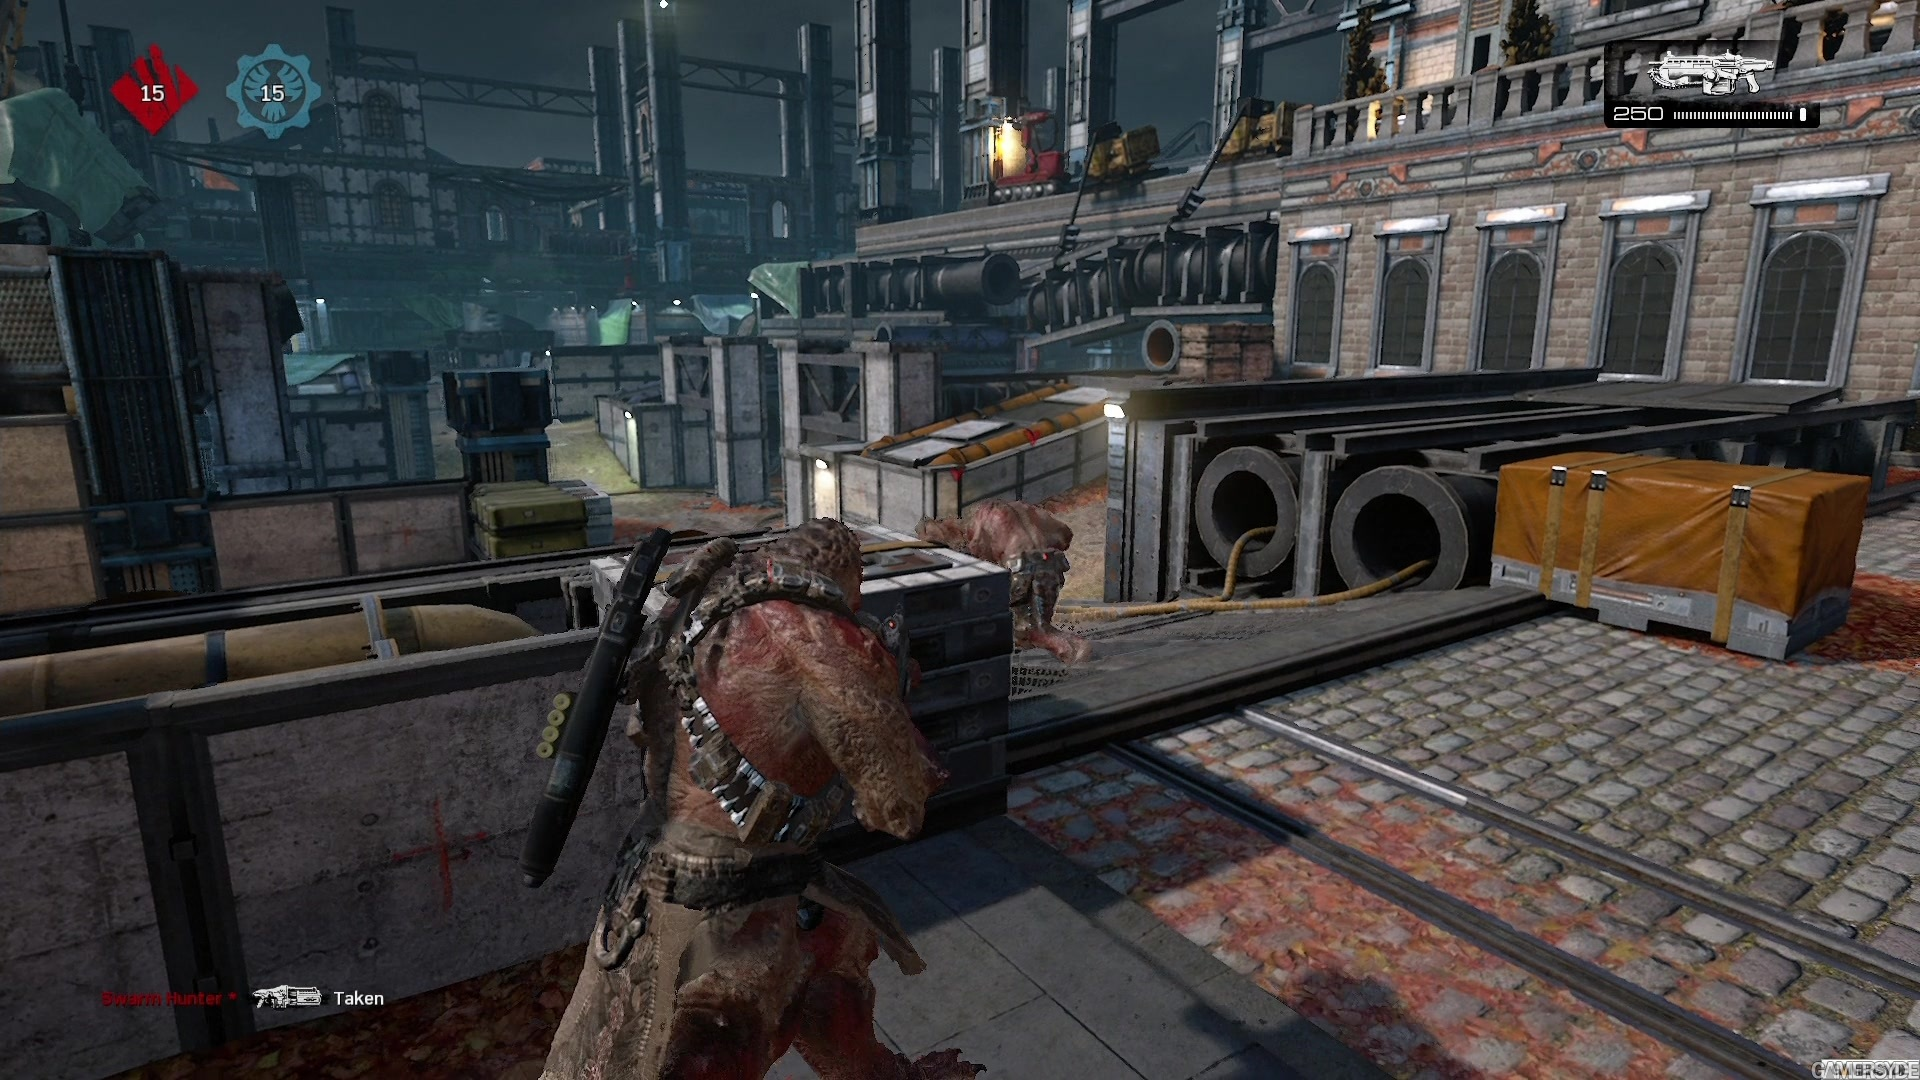
\includegraphics[width=\textwidth]{figures/ch1/gears}
			\caption[Le TPS \emph{Gears of War 4}]{Extrait du TPS \emph{Gears of War 4}. La caméra est placée derrière le personnage, au-dessus et sur le côté. Jeu développé par The Coalition et édité par Microsoft Studios.}
			\label{fig:gears}
		\end{subfigure}
		\caption{Jeux de tir.}
		\label{fig:shooters}
	\end{figure}
	
	Attendu que dans les FPS/TPS, la visée est précisément le cœur du jeu, et censée être difficile, les développeurs seraient probablement peu enclins à intégrer des techniques la facilitant, car cela diminuerait l'intérêt ludique de leur œuvre. Toutefois, cela pourrait avoir un intérêt dans le cadre d'un mode de jeu à difficulté réduite, pour les débutants. D'ordinaire, ces modes sont plutôt mis en œuvre par une réduction du nombre des ennemis, de leurs compétences, de leur résistance, etc., ce qui peut rendre l'expérience de jeu moins spectaculaire, ou moins cohérente avec le scénario.
	
	\subsection{Jeux de rôles (RPG)}
	Dans un jeu de rôle (RPG) classique, l'enjeu est très différent. Les capacités du (des) personnage(s) contrôlé(s) par le joueur dépendent de l'expérience accumulée depuis le début du jeu, l'expérience étant ici une ressource précisément quantifiée, sous forme de points la plupart du temps. Ces points sont ensuite investis dans des attributs (force, dextérité, endurance, intelligence\ldots{}) ou compétences (combat à mains nues, tir au fusil, persuasion, discrétion, magie de types divers\ldots{}). Souvent, les performances de visée d'un personnage dépendent uniquement de ses attributs et compétences, et non de la dextérité du joueur, qui n'a pas forcément besoin de désigner les cibles (le personnage les choisissant automatiquement) ou qui peut le faire pendant que l'action du jeu est en pause.
	
	Une assistance à la sélection pourrait ici permettre à l'utilisateur de désigner plus facilement des cibles pour ses personnages (afin d'outrepasser le choix fait automatiquement par le personnage, ce qui est parfois judicieux) ou de pouvoir le faire confortablement sans avoir à mettre le jeu en pause, ce qui a pour conséquence non seulement de ralentir le jeu --- et donc de faire perdre du temps au joueur --- mais aussi, potentiellement, de nuire à la sensation d'immersion. Il s'agirait dans ce genre d'accroître le confort des jeux, sans avoir à en altérer les mécanismes fondamentaux.
	
	\subsection{Jeux de rôle d'action (ARPG)}
	Mais il existe aussi une catégorie intermédiaire, les jeux de rôle d'action (ARPG). Les détails varient d'un jeu à l'autre, mais dans ce genre de jeux, le joueur est directement responsable des mouvements de ses personnages, tandis que les attributs et compétences du personnage ont une influence sur ses performances finales. Ce principe peut être mis en œuvre de diverses façons. En ce qui concerne le tir avec une arme, trois options, non mutuellement exclusives, sont couramment retenues :
	\begin{description}
		\item[Dispersion] Quand les compétences de tir du personnage sont faibles, le réticule de visée est agrandi, ce qui indique au joueur que l'angle du cône de dispersion\footnote{Ce cône représente le volume minimal dans lequel les trajectoires possibles des tirs sont contenues.} est grand. À mesure que les attributs et compétences du personnage augmentent, le réticule et le cône se resserrent.
		\item[Perturbations] Le curseur et le cône de dispersion peuvent être constants par rapport aux attributs et compétences, mais ils bougent même lorsque le joueur ne touche pas à son périphérique de saisie. Celui-ci doit donc compenser ces mouvements pour viser correctement. À mesure que les attributs et compétences du personnage augmentent, ces mouvements diminuent, voire disparaissent entièrement.
		\item[Recul] Une arme de jet a généralement un certain recul. Celui-ci a peu d'influence sur la précision du premier tir, mais plus sur les suivants. Dans un jeu vidéo, il est généralement simulé par un mouvement du curseur après le tir, habituellement vers le haut, avec en plus une composante horizontale, qui peut être aléatoire. On peut diminuer cet effet de recul quand les attributs et compétences du personnage croissent, éventuellement jusqu'à l'annuler totalement.
	\end{description}

	Ces mécanismes permettent d'obtenir une difficulté de tir qui dépend du joueur, puisqu'il doit tout de même viser, mais aussi des attributs et compétences du personnage. Il s'agit toujours de gêner le joueur, de lui imposer un handicap qui diminue quand les attributs et compétences de ses personnages augmentent. Mais \emph{in fine}, lorsque ce handicap est minime ou nul, le joueur reste borné par sa propre dextérité, comme dans un FPS classique.
	
	Une autre technique, utilisée par les récents opus de la série \emph{Fallout} appelée \emph{V.A.T.S.}, consiste à arrêter ou considérablement ralentir le temps, pour permettre au joueur de désigner ses cibles, que le personnage attaquera ensuite automatiquement. L'inconvénient majeur de cette solution (figure~\ref{fig:f4vats}) est la perte du temps-réel, et l'impact négatif sur l'immersion qui y est associé. De plus, le caractère automatique de l'attaque, une fois les cibles désignées, rend l'opération totalement indépendante de la dextérité du joueur, ce qui d'une part est une déviation par rapport au paradigme de l'ARPG, et d'autre part peut diminuer l'intérêt ludique du combat, ou nuire à la sensation d'immersion.
	
	\begin{figure}[!htbp]
		%\centering
		\begin{subfigure}[t]{0.48\textwidth}
			\centering
			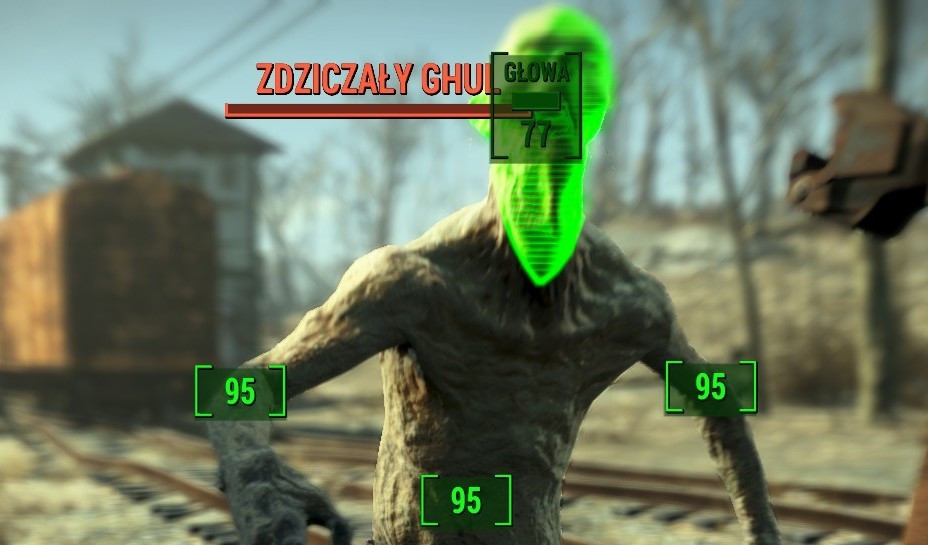
\includegraphics[width=\textwidth]{figures/ch1/f4vats}
			\caption[Système V.A.T.S permettant de faciliter les tirs dans \emph{Fallout 4}]{Dans l'ARPG \emph{Fallout 4}, le système V.A.T.S. permet ici au joueur de cibler tranquillement la tête de cette créature, pendant que le temps est ralenti. Le tir aura une probabilité de succès de 77~\%{}, dérivée des compétences de tir du personnage contrôlé, et des circonstances du combat à cet instant précis. Jeu édité par Bethesda Softworks, et développé par ses propres studios.}
			\label{fig:f4vats}
		\end{subfigure}
		~
		\begin{subfigure}[t]{0.50\textwidth}
			\centering
			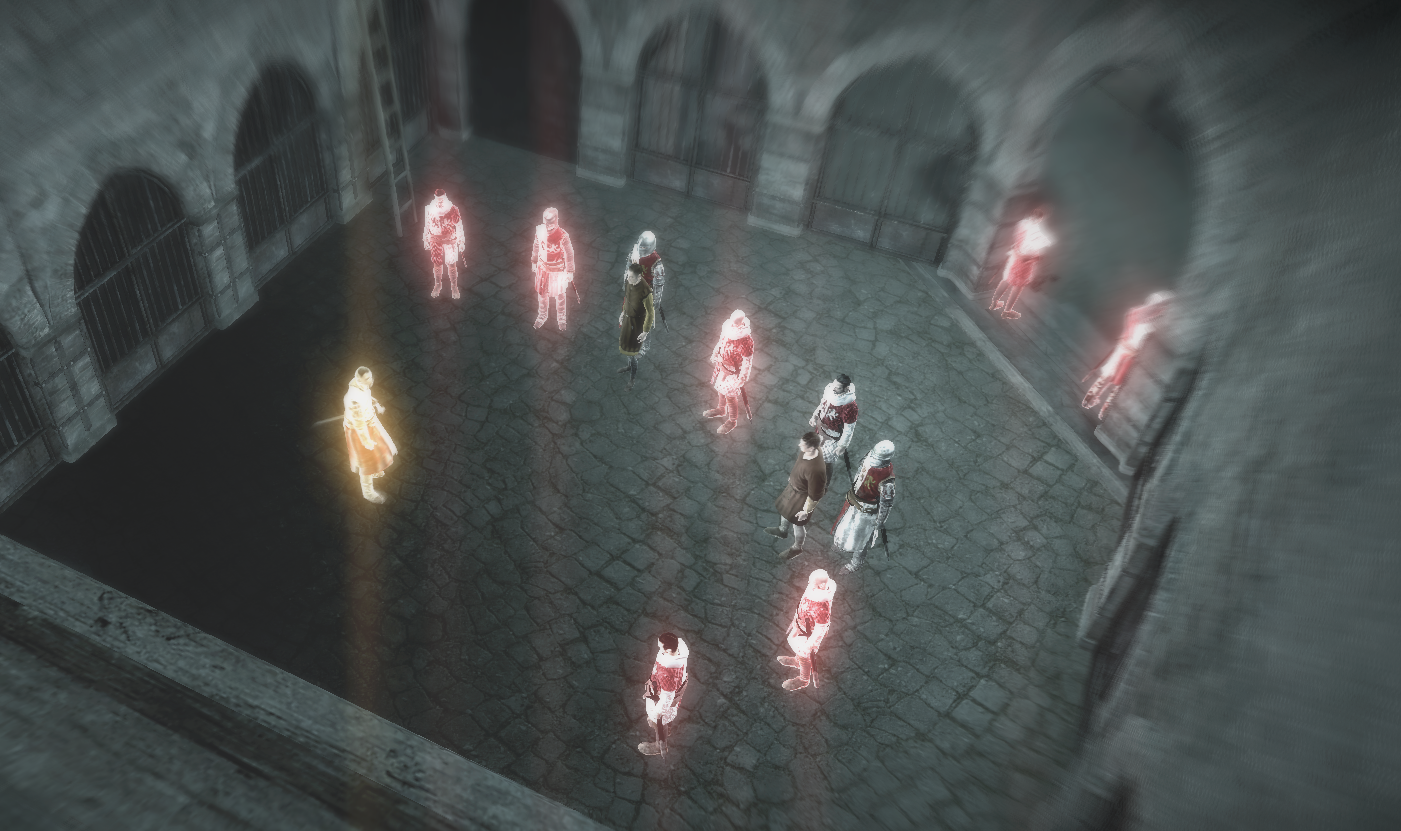
\includegraphics[width=\textwidth]{figures/ch1/assassin}
			\caption[Système \emph{Eagle Vision} dans le jeu \emph{Assassin's Creed}] {\emph{Assassin's Creed} : le joueur peut voir les personnages à travers les obstacles, connaître leur nature grâce à leur couleur, et désigner la cible que le personnage attaquera ensuite semi-automatiquement. Si les cibles elles-mêmes ne sont ni très rapides ni très imprévisibles, à leurs mouvements absolus s'ajoutent ceux du joueur, qui ne dispose généralement que d'un petit \emph{joystick} sous son pouce pour viser. Édité et développé par Ubisoft.}
			\label{fig:ac_ev}
		\end{subfigure}
		\label{fig:gamesTargeting}
		\caption{Techniques d'assistance à la visée ou sélection dans les jeux vidéo.}
	\end{figure}
	
	On pourrait imaginer, à la place ou en complément de ces approches, d'apporter au joueur une assistance à la visée. Une telle technique d'aide à la sélection devrait être paramétrable dans son \og intensité \fg{} c'est-à-dire qu'il devrait lui être possible d'apporter au joueur une assistance plus ou moins prononcée, selon un paramètre donné. Ce paramètre pourrait être (dérivé de) la compétence de tir du personnage. Ainsi, un joueur contrôlant un personnage expert en tir serait capable d'abattre des cibles très difficiles, conformément à l'image du personnage telle qu'elle est véhiculée par le jeu, mais le joueur resterait l'acteur principal de l'opération, sans ralentissement ou suspension du temps. L'aide à la sélection permettrait ici de dépasser la \og borne \fg{} imposée par la dextérité du joueur.
	
	À l'inverse, sans aide à la sélection, même un joueur très adroit aurait du mal à abattre ses cibles si les attributs et compétences de son personnage étaient faibles, car il serait dépourvu d'assistance, et pourrait être handicapé par une (ou plusieurs) des méthodes mentionnées plus haut. Un tel système permettrait d'obtenir des performances de tir qui dépendraient toujours significativement de l'adresse du joueur, mais qui demeureraient en accord avec les performances attendues de la part d'un personnage donné en fonction de ses attributs et compétences, et donc maintiendraient la cohérence de l'univers du jeu tel qu'envisagé par ses créateurs.	
	
	\subsection{Jeux de gestion, de stratégie (RTS) et de tactique (RTT)}
	Dans ce que nous appellerons, pour simplifier, les jeux de gestion (en y incluant la catégorie \emph{Real-time strategy} ou RTS, et \emph{Real-time tactics} ou RTT) le but est de mener un organisme (d'une petite entreprise à une civilisation) vers la prospérité, ou une armée vers la victoire. Ces genres mettent l'accent sur la réflexion tactique et stratégique, la gestion des ressources naturelles et humaines, l'organisation logistique, etc.

	\begin{figure}[!htbp]
		\begin{subfigure}[t]{\textwidth}
			\centering
			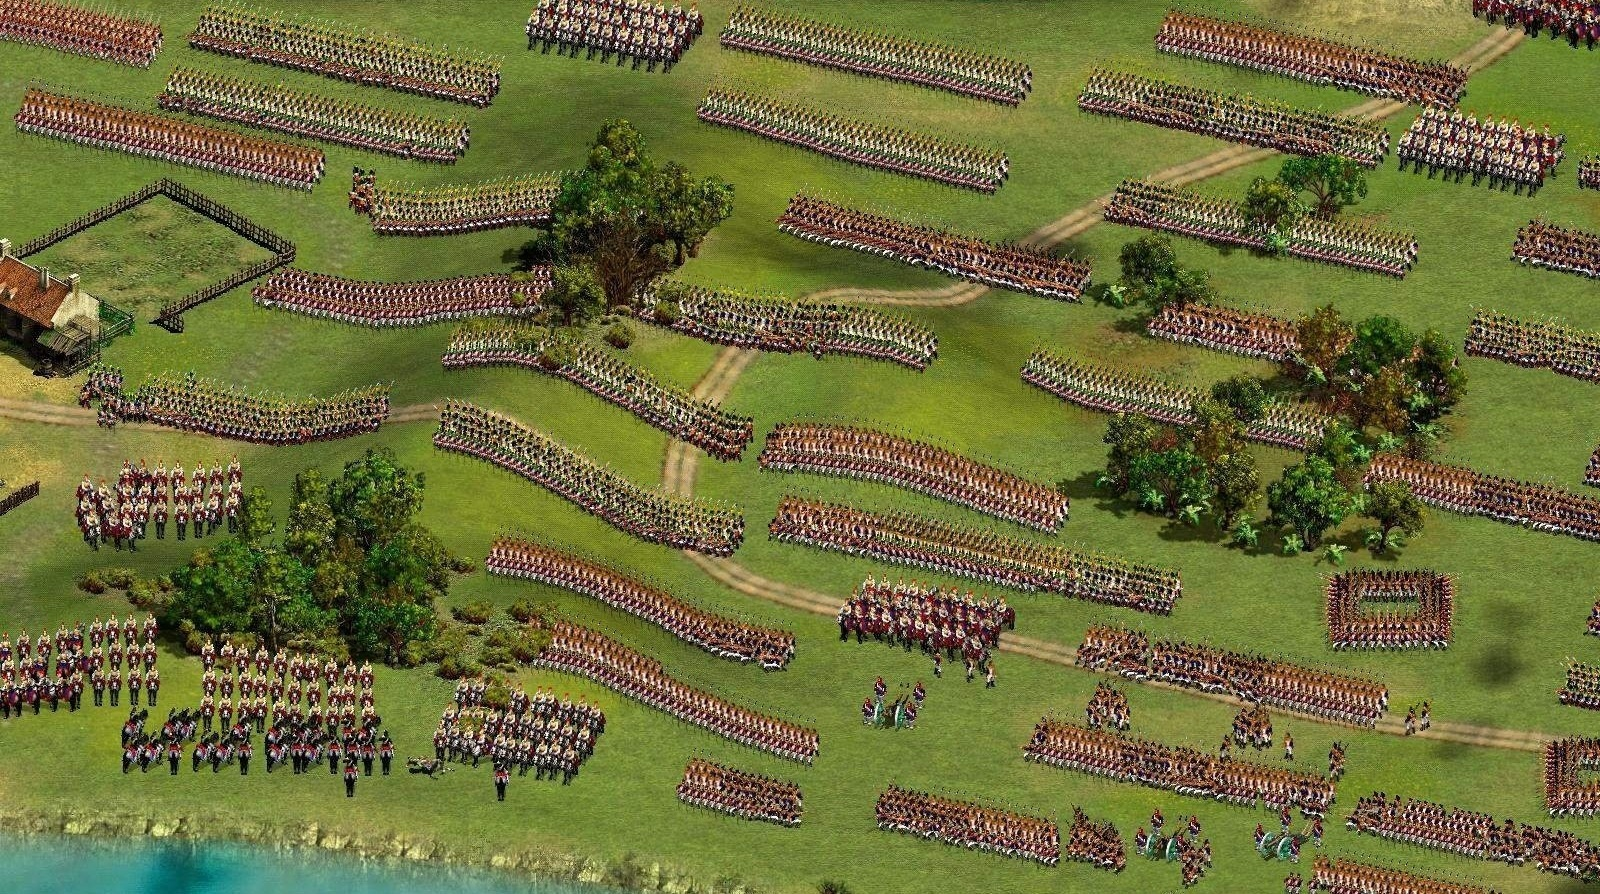
\includegraphics[width=\textwidth]{figures/ch1/cossacks2}
			\caption[Un RTS avec de très nombreuses unités : \emph{Cossacks~II: Napoleonic Wars}]{\emph{Cossacks~II: Napoleonic Wars} : les unités sont nombreuses, très proches les unes des autres. Au nombre et à la densité s'ajouteront, pendant la bataille, le mouvement, le désordre et le mélange avec des unités ennemies. Développé par GSC Game World et édité par CDV Software.}
			\label{fig:cossacks2}
		\end{subfigure}
		~
		\begin{subfigure}[t]{\textwidth}
			\centering
			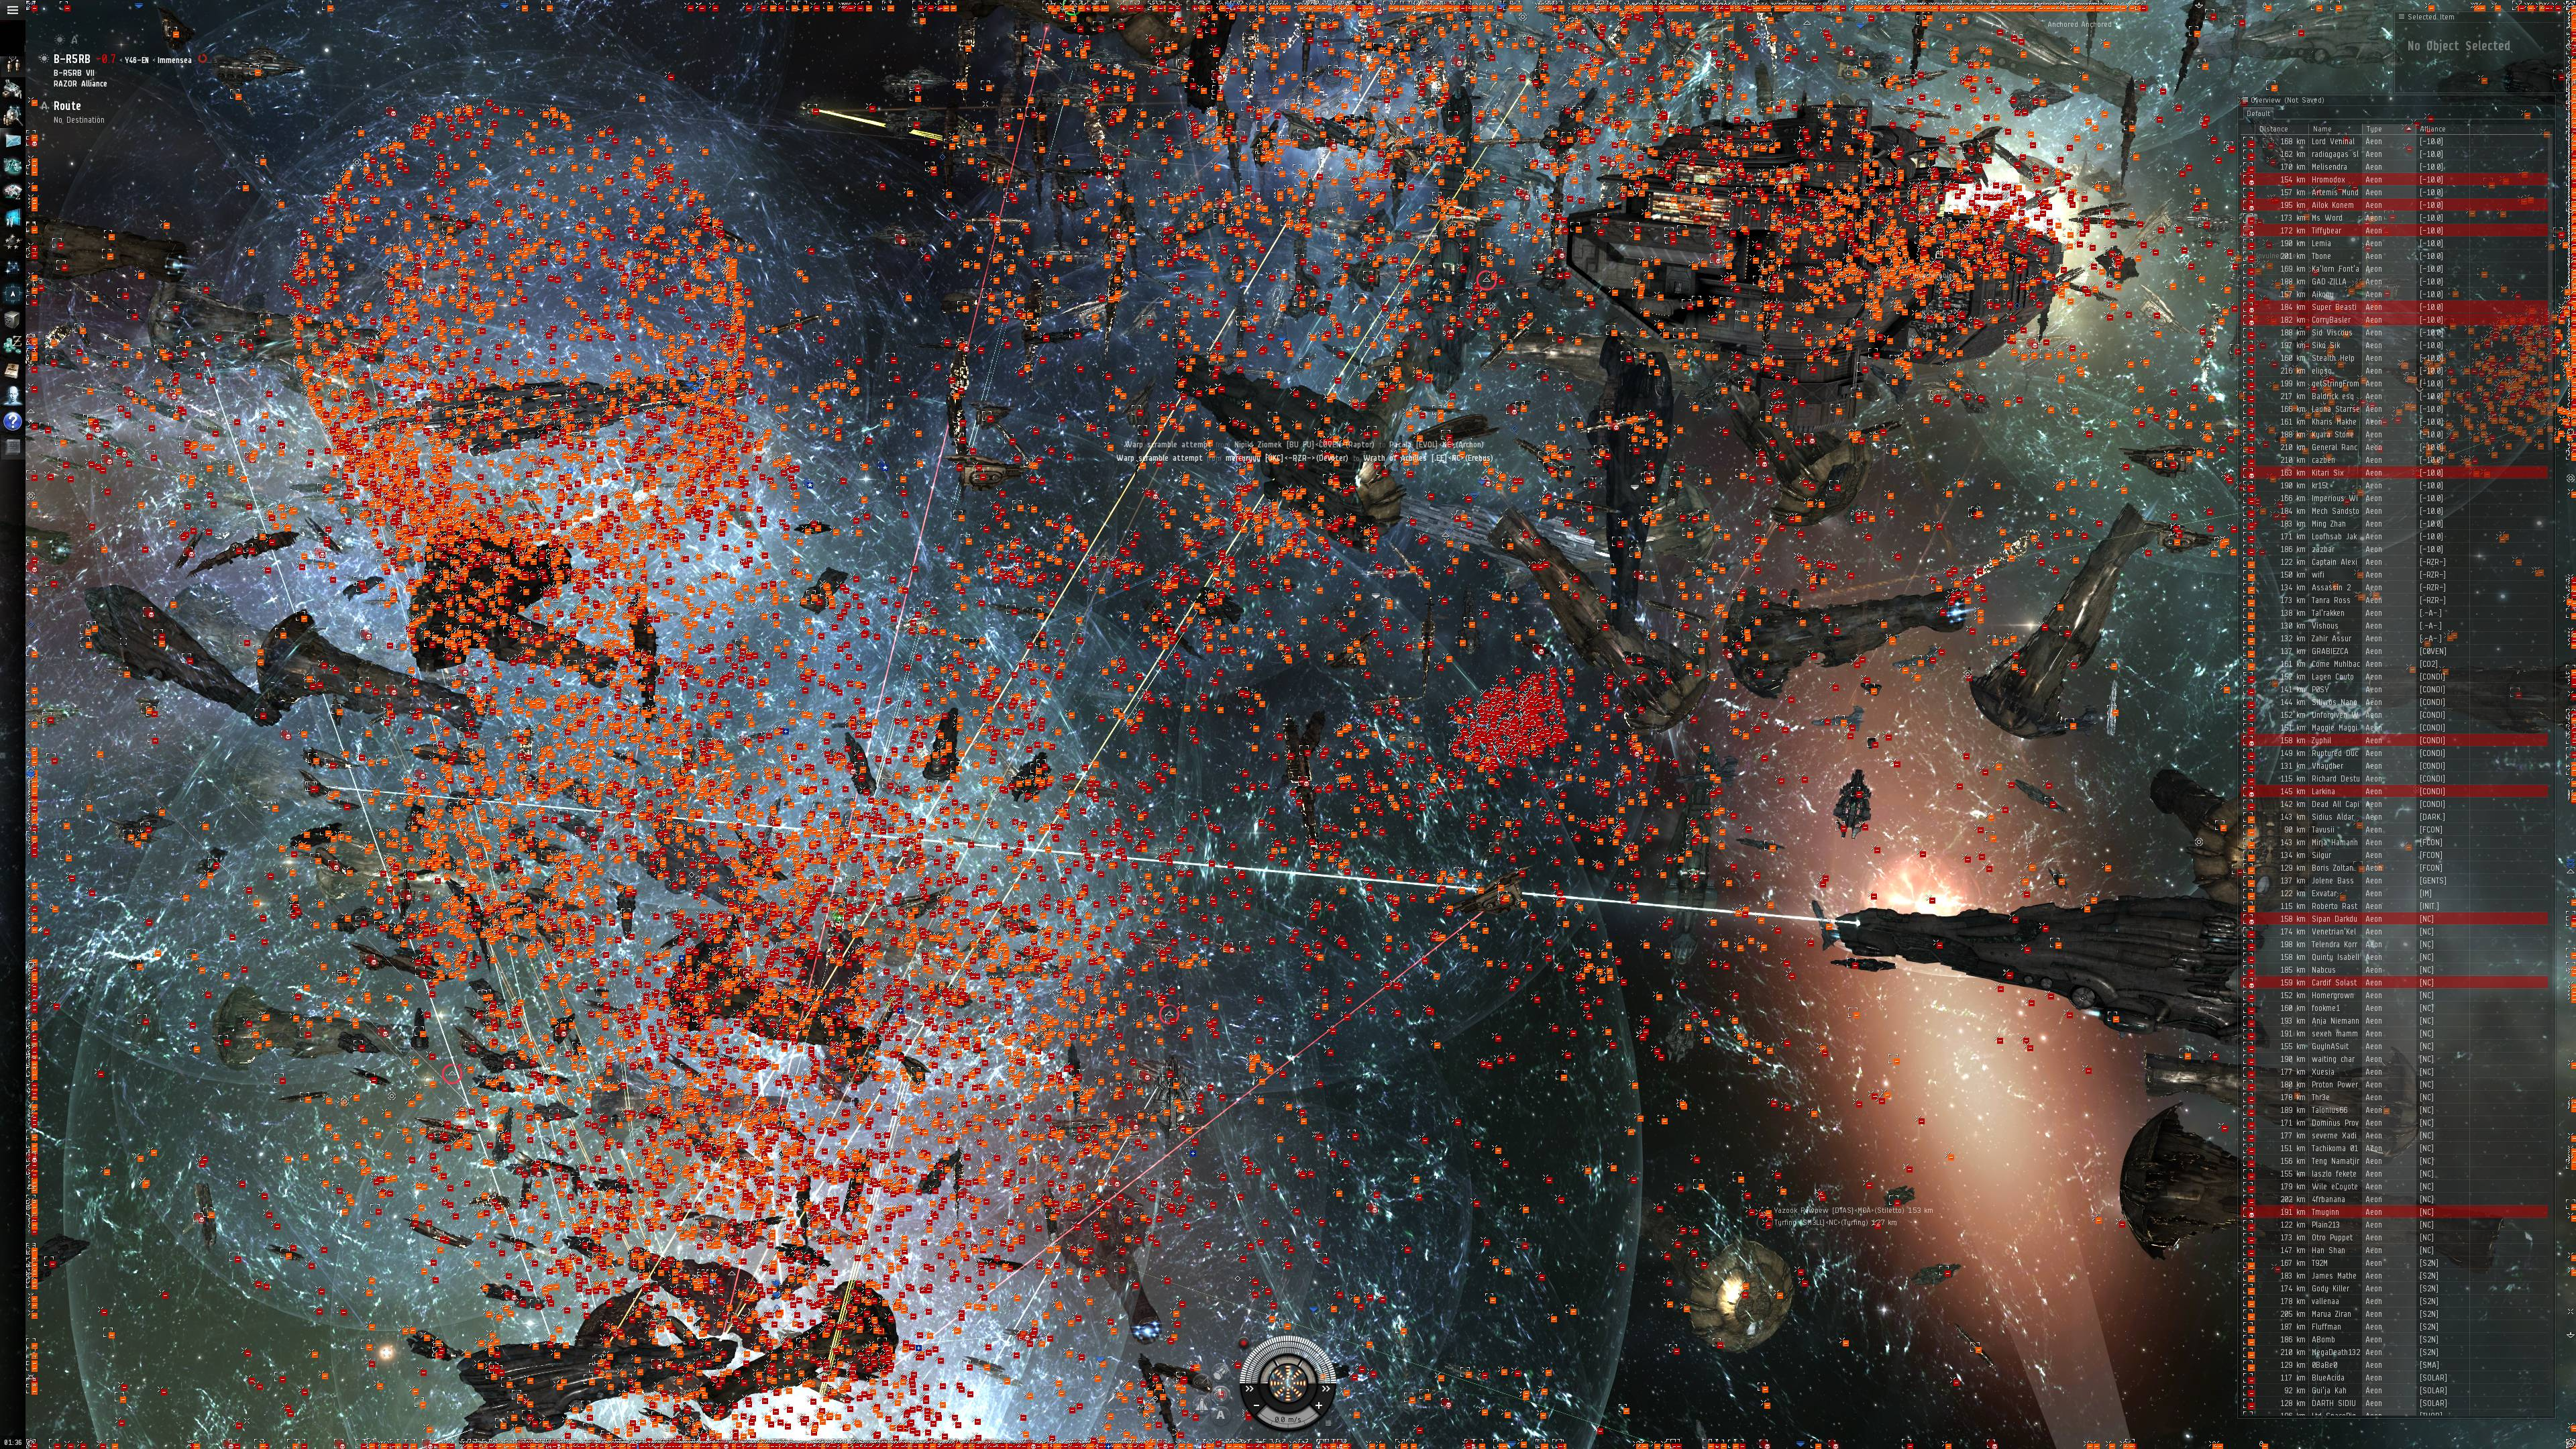
\includegraphics[width=\textwidth]{figures/ch1/eveonline}
			\caption[Énorme bataille dans le jeu \emph{EVE Online}]{Énorme bataille dans le jeu \emph{EVE Online}. Le nombre précis d'unités est inconnu, mais chaque point rouge ou orange représente un vaisseau ou un drone, donc une cible potentielle. Crédit : \emph{EVE Online Community} ; développé et édité par CCP Games.}
			\label{fig:eveonline}
		\end{subfigure}
		\caption[Jeux de stratégie]{Jeux de stratégie.}
		\label{fig:stratGames}
	\end{figure}

	S'il est fréquemment nécessaire de sélectionner des cibles dans ces jeux, ce n'est pas une fin en soi, ou un objectif conçu comme ayant une valeur ludique. Il s'agit de sélectionner des unités amies pour leur donner des instructions, ou des unités ennemies pour les désigner comme cibles à attaquer. Au contraire, la tâche de sélection est purement utilitaire et vue comme une nécessité, voire une corvée. Elle fait perdre du temps au joueur, du temps qui pourrait être utilisé pour organiser ses ressources, ou tout simplement pour réfléchir.
	
	Par conséquent, une technique de sélection facilitant cette tâche serait bénéfique en recentrant ces jeux sur leurs cœurs. Dans les jeux de gestion, les cibles peuvent être extrêmement nombreuses. Dans  \emph{Cossacks~II: Napoleonic Wars}, par exemple, une bataille peut engager jusqu'à 64~000 unités, et la situation devient assez délicate à gérer pour pousser les joueurs à mettre le jeu en pause, le temps de donner des instructions aux unités\footnotemark. Il est évident que si cette solution est acceptable (quoique loin d'être idéale) dans un jeu opposant une intelligence artificielle au joueur, elle vient beaucoup plus gênante dans un contexte multijoueur, où les instances du jeu s'exécutant sur chaque machine doivent rester synchronisées. Une bataille de ce jeu est illustrée par la figure~\ref{fig:cossacks2}, mais elle est eclipsée par l'énorme bataille du jeu multijoueur \emph{EVE Online} (figure~\ref{fig:eveonline}).
	
	\footnotetext{\emph{Cossacks~II: Napoleonic Wars -- Strategy Guide} --- \url{http://www.ign.com/articles/2005/05/27/cossacks-ii-napoleonic-wars-strategy-guide}}
	
	S'il est parfois souhaitable de sélectionner \emph{une} unité, il est plus fréquent de vouloir en sélectionner un groupe d'un coup. Une technique de sélection appropriée devrait donc impérativement préserver cette possibilité. Une telle technique allégerait le fardeau de la sélection, laissant les joueurs se concentrer sur les éléments ayant une valeur ludique --- gestion, tactique et stratégie, etc. Elle pourrait même permettre de gérer des situations plus complexes, avec plus d'unités, plus de variables à prendre en compte, et donc plus de richesse tactique ou stratégique. De fait, l'on pourrait s'approcher un peu plus des situations réelles que ces jeux simulent parfois --- la bataille de Stalingrad, par exemple, impliquait quelque deux millions d'hommes, sans compter le matériel.

	\subsection{Arènes de bataille en ligne multijoueur (MOBA/ARTS)}
	Les jeux de type arène de bataille en ligne (MOBA, ou ARTS pour \emph{action real-time strategy}) ont émergé comme un sous-genre de la catégorie RTS, dans lequel le joueur ne contrôle qu'un seul personnage, et est éventuellement aidé par des personnages non jouables\footnotemark{} dans sa lutte contre ses ennemis. Ces derniers sont souvent au nombre d'une poignée ou de quelques dizaines, et sont généralement caractérisés par leurs mouvements vifs. Les MOBA présentent donc un assez petit nombre de cibles potentielles (parfois très) rapides dont les mouvements sont fréquemment imprévisibles. Le jeu \emph{League of Legends} est un exemple de MOBA, illustré par la figure~\ref{fig:lol}.
	
	\footnotetext{PNJ : personnage non jouable, ou non-joueur, de l'anglais \emph{non-player character} (NPC). Désigne, dans un jeu vidéo, un personnage contrôlé exclusivement par l'ordinateur, qui peut être opposé au joueur, l'aider, ou avoir une position neutre.}
	
	\begin{figure}[!htbp]
		%\centering
		\begin{subfigure}[t]{0.52\textwidth}
			\centering
			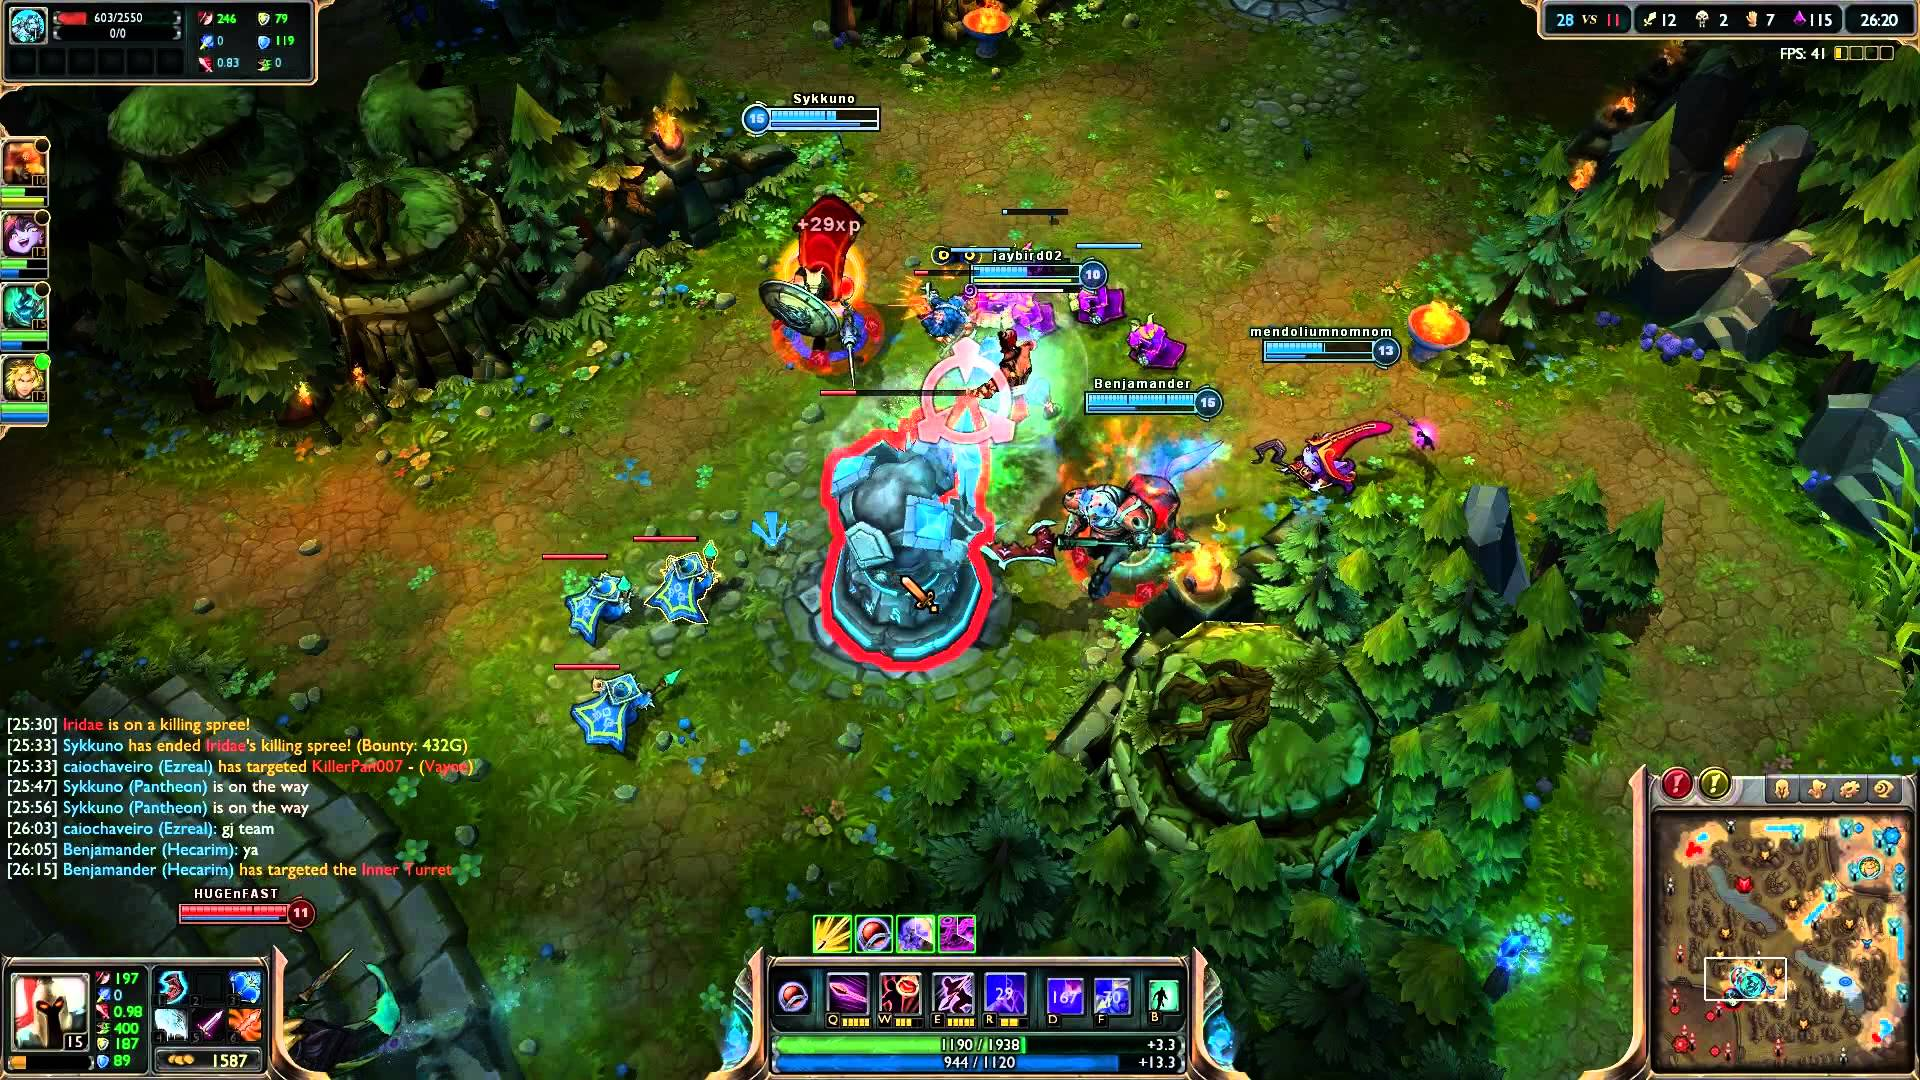
\includegraphics[width=\textwidth]{figures/ch1/lol}
			\caption[Une partie du MOBA \emph{League of Legends}]{\emph{League of Legends}, de Riot Games.}
			\label{fig:lol}
		\end{subfigure}
		~
		\begin{subfigure}[t]{0.46\textwidth}
			\centering
			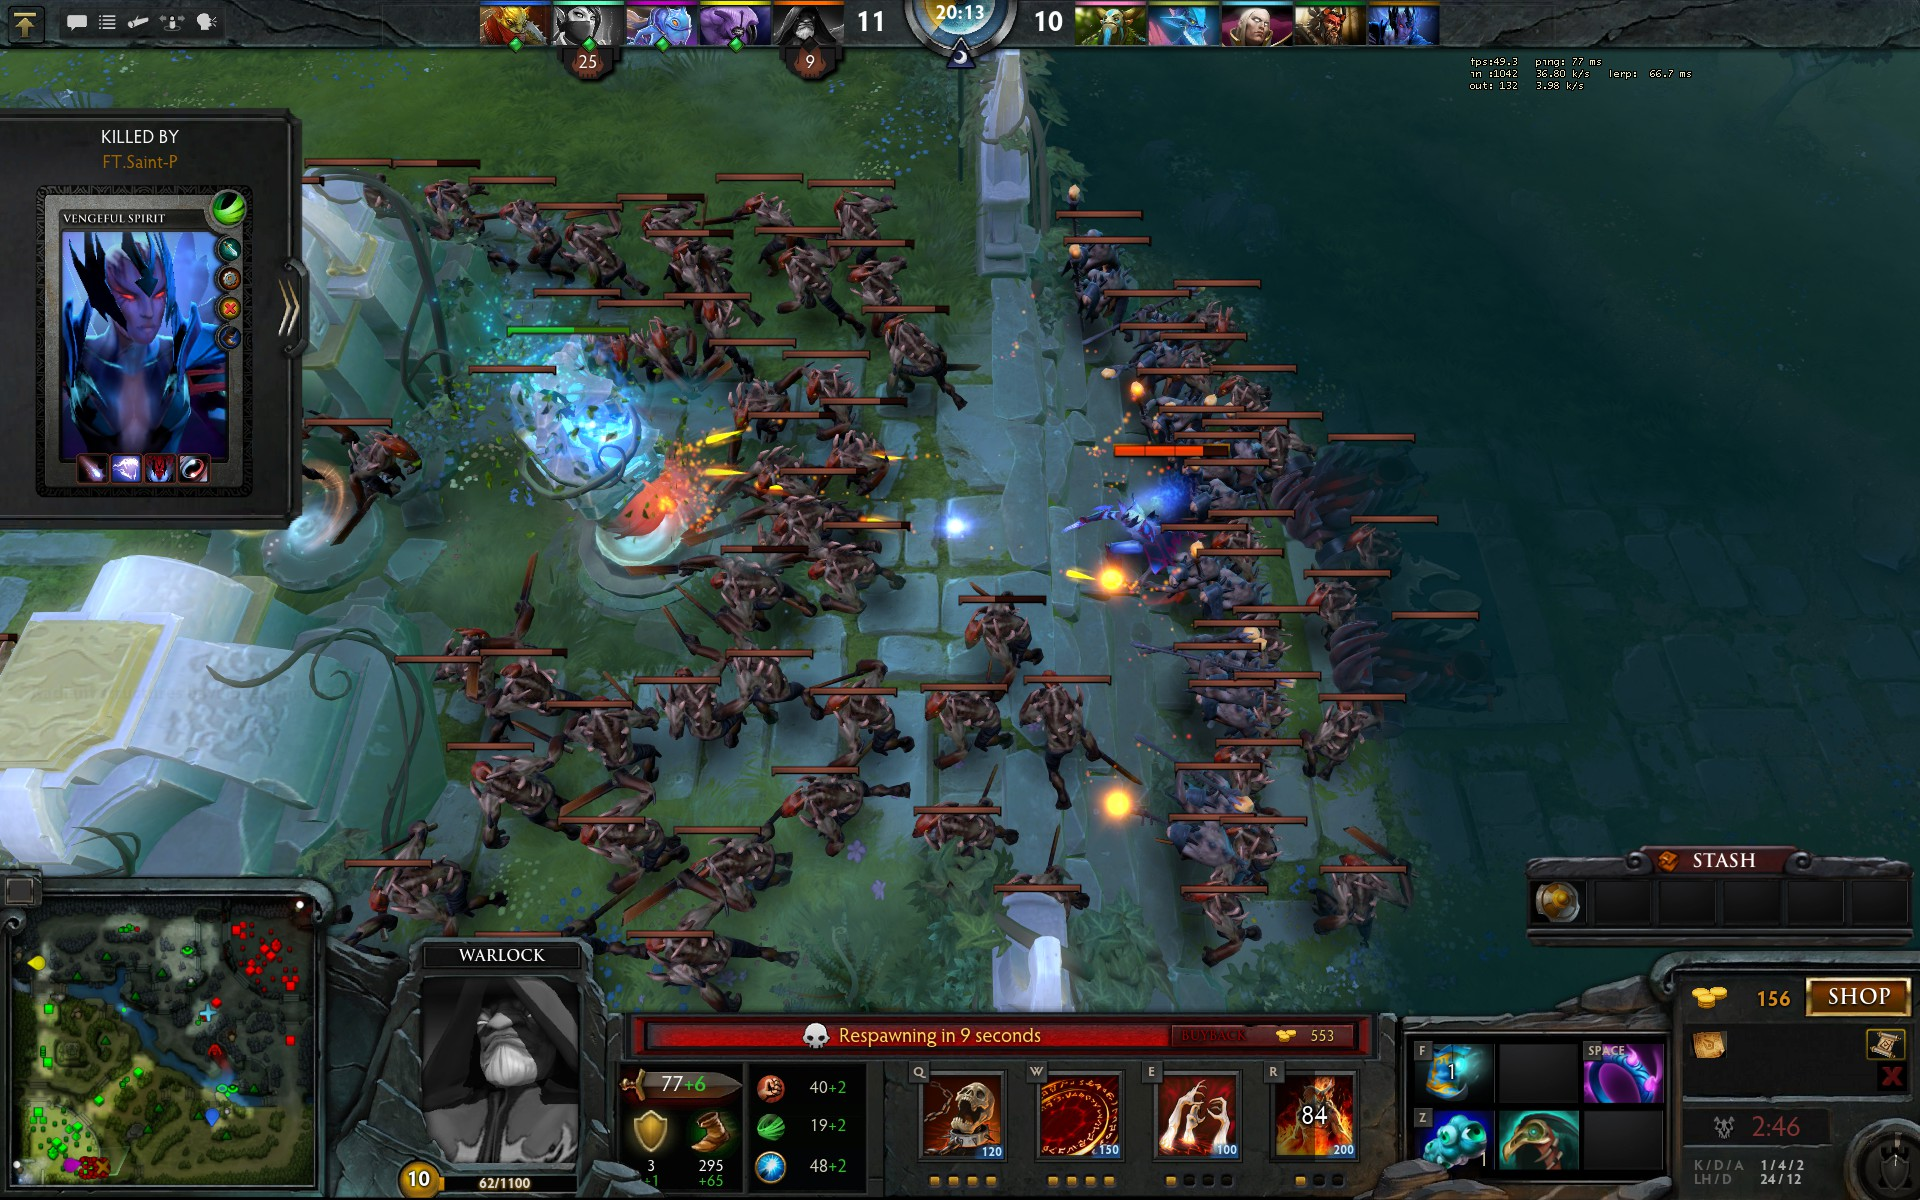
\includegraphics[width=\textwidth]{figures/ch1/dota2}
			\caption[Une partie d'un MOBA, \emph{DOTA~2}]{\emph{DOTA~2}, de Valve Corporation.}
			\label{fig:dota2}
		\end{subfigure}
		\label{fig:mobas}
		\caption[Arènes de bataille en ligne multijoueur (MOBA)]{Arènes de bataille en ligne multijoueur (MOBA). Les objets sont peu nombreux, mais leurs mouvements sont vifs, imprévisibles, et divers événements peuvent créer des effets visuels occultant une partie de l'écran. Pour autant, le jeu ne s'arrête pas pendant ces moments-là et il demeure nécessaire de pouvoir sélectionner des personnages.}
	\end{figure}

	Le \emph{wiki} du MOBA \emph{Dota~2} fournit des informations très précises sur les caractéristiques de mouvement des unités principales du jeu\footnotemark{}. Celles-ci sont reproduites dans le tableau~\ref{tab:dotamoves}. Les détails figurent dans la légende du tableau, mais l'on peut résumer ces informations en deux points essentiels : les personnages peuvent changer de direction de façon significative à une fréquence de plusieurs dizaines de hertz, et ils peuvent se déplacer d'une dizaine de centimètres par seconde sur l'écran du joueur. Ces changements de direction se font au gré des décisions de l'intelligence artificielle pour les PNJ, ou du joueur pour les personnages qu'il contrôle. \emph{Dota~2} est un jeu multijoueur, et naturellement les joueurs peuvent chercher à éviter les attaques de leurs adversaires, précisément en adoptant des mouvements imprévisibles.
	
	Par conséquent, une technique d'aide à la sélection serait bénéfique dans le sens où elle permettrait aux joueurs de se concentrer sur les aspects tactiques du jeu, mais elle pourrait également modifier l'équilibre du jeu en faveur de l'attaque, au détriment de l'esquive. Cette perturbation de l'équilibre ne serait pas nécessairement souhaitable, mais elle pourrait aussi être compensée par une augmentation de la vitesse des personnages. Le résultat net serait donc d'augmenter la sensation de vivacité du jeu. Une autre option serait de permettre aux personnages, actuellement limités à un espace bidimensionnel, d'évoluer en 3D. Une assistance à la sélection suffisamment performante permettrait d'acquérir les cibles souhaitées même en 3D, ce qui conférerait une toute nouvelle profondeur tactique au genre MOBA.
	
	\footnotetext{\emph{Dota~2 Wiki -- Turn rate} --- \url{http://dota2.gamepedia.com/Turn_rate}}
	
	\newcommand{\newrow}{\bigstrut[t] \\ \hline}
	\newcolumntype{Y}{>{\small}X}
	\newcolumntype{Z}{>{\centering}X}
	\begin{table}[!htbp]
		\centering
		\begin{tabularx}{\textwidth}{ Y X X X } % Putain j'entrave que dalle mais ça marche à peu près
		Héros				&	Temps de demi-tour (s)	&	Vitesse (u.a.)	&	Vitesse affichée (cm/s)	\newrow
		Lifestealer			&	0.094 s					&	315				&	63						\newrow
		Shadow Fiend		&	0.094 s					&	315				&	63						\newrow
		Magnus				&	0.118 s					&	315				&	63						\newrow
		Luna				&	0.157 s					&	335				&	67						\newrow
		Keeper of the Light	&	0.188 s					&	335				&	67						\newrow
		Pugna				&	0.188 s					&	330				&	66						\newrow
		Enchantress			&	0.236 s					&	335				&	67						\newrow
		\og Maximum \fg{}	&	---						&	550				&	110						\newrow
		\end{tabularx}
		\caption[Caractéristiques de mouvement des personnages vifs de \emph{Dota~2}]{Caractéristiques de mouvement des personnages les plus vifs de \emph{Dota~2}. Les plus \og agiles \fg{} peuvent effectuer un demi-tour en moins de 0,1~s, soit une fréquence d'un peu plus de 10~Hz, ou 20~Hz pour des virages de 90\textdegree, 30~Hz pour 60\textdegree, etc. Les vitesses des personnages sont notées dans les unités arbitraires du jeu (u.a.), et en cm/s telles qu'elles apparaissent sur un écran (en supposant un écran de bureau de taille et de définition courantes). La ligne \emph{Maximum} correspond à la vitesse \og maximale \fg{} d'un personnage --- en pratique, des objets ou capacités accessibles à certains personnages leur permettent d'aller encore plus vite.}
		\label{tab:dotamoves}
	\end{table}
	% On peut considérer que 128 unités représentent à peu près un mètre dans l'espace virtuel, et apparemment 600 unités feraient environ 12 cm à l'écran, soit environ 2 mm par unité.
	% https://www.hiveworkshop.com/threads/warcraft-iii-distance-units-convert.137848/
	% https://www.reddit.com/r/DotA2/comments/1vaklc/how_big_is_the_dota2_map_really/
	
	\FloatBarrier \subsection{Richesse et diversité}
	L'univers vidéoludique est d'une richesse et d'une diversité considérables tandis que le nombre de jeux est considérable et constante croissance. 
	
	Il serait bien impossible dans ce manuscrit de faire un inventaire complet de cette diversité, dût-il être entièrement consacré à cet objectif. Pour illustrer cette richesse et cette diversité, contentons-nous simplement de mentionner un seul exemple, \emph{Agar.io}. Dans cette curieuse création de Matheus Valadares, le joueur contrôle un disque coloré qu'il doit nourrir pour le faire grossir au maximum, en dévorant ses adversaires.
	
	Le principe de ce jeu d'une complexité inattendue est illustré par la figure~\ref{fig:agario}. Pour avaler un adversaire, l'on peut soit le rattraper et l'englober, ce qui est difficile car il faut pour cela être significativement plus gros (et donc plus lent, selon le mécanisme du jeu) soit se diviser en deux et propulser une de ses moitiés sur lui, ce qui nécessite de viser très soigneusement, et d'autant plus prudemment qu'une fois scindé en deux, le joueur est beaucoup plus vulnérable à ses gros adversaires.
	
	\begin{figure}[!htbp]
		\centering
		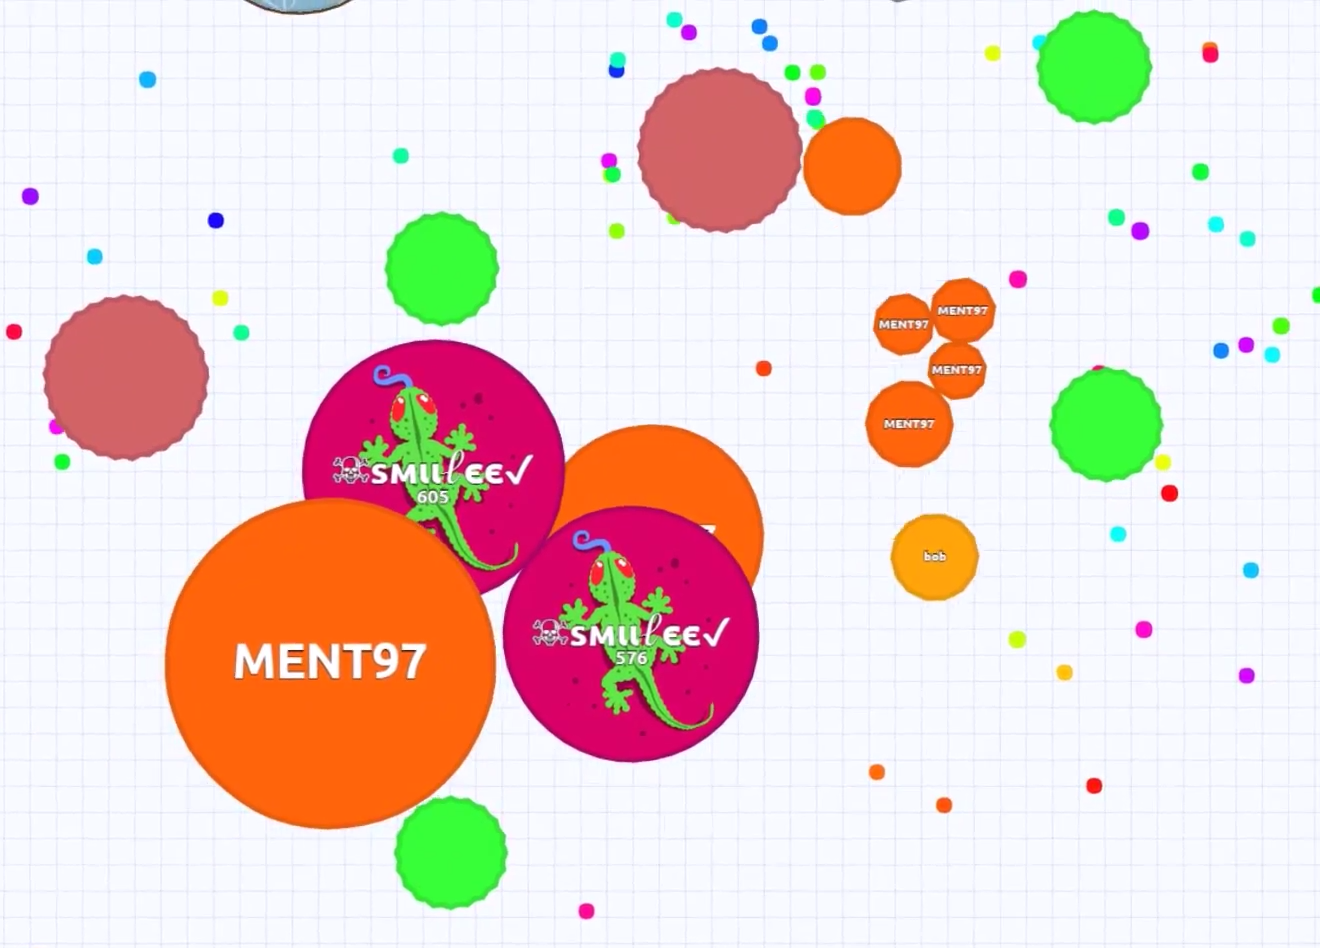
\includegraphics[width=0.56\textwidth]{figures/ch1/agario}
		\caption[\emph{Agar.io}]{\emph{Agar.io} : chaque ensemble de disques d'un même nom est contrôlé par un joueur, qui cherchera à dévorer les autres disques. Ceux à bords dentés sont des obstacles causant l'éclatement des joueurs qui les percutent vivement. Chaque petit disque sans texte est de la nourriture à attraper. Dans cette scène, les cibles sont nombreuses et leur agancement est complexe, d'autant qu'elles sont contrôlées par des humains qui cherchent à s'abriter derrière les obstacles. Crédit : GD Rentstr0m\footnotemark{} ; développé et édité par Matheus Valadares.}
		\label{fig:agario}
	\end{figure}
	
	\footnotetext{\url{https://www.youtube.com/watch?v=XaZ2n_feTko}}
	
	Sans doute \emph{Agar.io} fait-il partie des jeux pour lesquels la visée est une fin en soi, un ressort ludique. Cependant, son principe très simple cache une profondeur tactique insoupçonnée, notamment du fait de la possibilité de coopérer avec d'autres joueurs, selon des procédés complexes --- bien qu'issus de mécanismes très simples --- qu'il n'est pas utile de détailler ici. Disons simplement que le développeur pourrait choisir de faciliter la visée pour mettre plus de poids sur la tactique.

	
	\section{Conclusion}    
	Les besoins en sélection de cibles mobiles sont très divers, et répartis sur des domaines variés : des simulations scientifiques aux jeux vidéo, en passant par le maintien de l'ordre, la défense, les retransmissions sportives, etc. Selon les domaines, les impératifs peuvent varier : dans tous les cas, la performance est recherchée, mais le temps de sélection peut être plus important pour certaines applications, et le taux d'erreur pour d'autres. Parfois, les applications sont si critiques que le temps de sélection doit impérativement être court et borné.
	
	La difficulté de la tâche de sélection de cible mobile varie également selon l'application. Voici les principaux facteurs de difficulté :
	\begin{itemize}
		\item la taille des cibles et leur distance par rapport au \og curseur \fg{} ou périphérique,
		\item la vitesse des cibles,
		\item la quantité absolue et la densité de cibles, le niveau d'occultation qui en découle,
		\item le nombre de dimensions de l'espace des cibles,
		\item l'hétérogénéité des cibles,
		\item la nature du mouvement, plus ou moins imprévisible.
	\end{itemize}
	
	Un examen des cas évoqués dans ce chapitre, mené à la lumière des facteurs sus-cités, suggère que les simulations de dynamique moléculaire interactives représentent la tâche la plus difficile, quoique certaines autres ne soient pas très loin derrière. Cette application peut donc servir de guide dans la conception d'une technique de sélection de cibles mobiles, à condition de maintenir une généricité suffisante.
	
	Cependant, compte tenu des divers impératifs requis par chaque application, une technique idéale devrait être suffisamment paramétrable pour favoriser le temps de sélection ou le taux d'erreur, selon les besoins. Elle devrait également pouvoir s'adapter à des espaces à deux et trois dimensions, ainsi qu'à des dispositifs de visualisation et d'interaction aussi divers que possible : téléphones (\emph{smartphones}), tablettes tactiles, ordinateurs portables équipés de \emph{touchpads}, ordinateurs de bureau équipés d'une souris et d'un clavier, dispositifs immersifs (de type CAVE ou HMD, par exemple), murs d'écrans, manettes de jeu, \emph{joysticks}, souris 3D, \emph{Flysticks}\footnotemark, bras haptiques, etc.
	
	\footnotetext{Périphérique d'interaction sans fil conçu pour la réalité virtuelle, produit par Advanced Realtime Tracking (ART) : \url{http://www.ar-tracking.com/products/interaction/flystick2}}
	
	L'enjeu des ces travaux de thèse est d'une part de formaliser le mouvement et la dynamique de ces cibles, en identifiant des facteurs de difficulté, tels que l'imprévisibilité du mouvement d'une cible, comme dans le cas de la simulation moléculaire. D'autre part, il s'agit de déterminer dans quelle mesure ces facteurs influencent les difficultés liées à sélection de cibles mobiles, problématiques à ce jour peu étudiées d'un point de vue expérimental. Ce travail préalable est essentiel pour répondre aux besoins des applications évoquées dans ce chapitre, comme base au développement de techniques pour faciliter la sélection de cibles mobiles.
	
	En amont, nous allons dans le chapitre suivant présenter un état de l'art des techniques de sélection de cibles.